% \providecommand{\main}{..} 

\documentclass[../main.tex]{subfiles}
\graphicspath{{\subfix{../figures/}}}
\usepackage{bbm}
% \addbibresource{../bibliography/bibliography.bib} % 

\begin{document}

    \chapter{State of the Art} \label{chap:state_of_the_art} \info{10-12 pgs}

    The following chapter provides an overview of the current environment and state of the art in the topics related to this work. The goal is to provide a better understanding of the techniques that can be used to address the problem introduced in the previous chapter, highlighting emerging methods and their relevance to the problem.
    
    We begin with a review of prior studies relevant to the topics of this thesis that have achieved state-of-the-art performance or have done similar work as the one proposed here. We go into detail about the implementation of the techniques used in each study, their overall contributions to the field, and how they relate to our work.
    
    Then, in section \ref{sec:relevant_techniques}, we give a high-level description of known machine learning paradigms and techniques that have been proposed in the literature to address continual adaptation and the degradation of ML systems deployed to real-world scenarios, highlighting their application in the healthcare domain.

    % Finally, we conclude the chapter with table \ref{tab:sota_summary}, which lists the studies discussed in this chapter that we consider to be the most relevant to our work. 
    
    % This table may serve as a reference for the following chapters, as it will be used to compare the contributions of this work to the state of the art.
    
    \section{Literature Review} \label{sec:literature_review} \todo{4-5 pages}

    This section provides a detailed overview of the most relevant work in the literature related to the topics of this thesis. It is meant for readers who want to dive more into the details of the techniques studied, how they achieved state-of-the-art performance, their overall contributions, and how they relate to the problems posed in this work.

    \subsection{Computer Vision and DL-Based Object-Detection Techniques } \label{sec:computer_vision_sota}

    This thesis focuses on applying computer vision (CV) techniques to the detection of Tuberculosis. Thus, we consider it essential to give an overview of the most important work in the literature in CV with the goal that the discussion here also serves as a good reference for the proposed solution and the techniques that will be introduced in the upcoming sections. 
    
    Since CV is a vast field, we cannot cover all the relevant work in the literature. Instead, since the problem in this work relates more to the tasks of image classification and object detection using Deep Learning (DL) algorithms (to identify Tuberculosis), we will limit our scope to the most relevant work in those areas.

    First, it's important to highlight the importance of DL techniques in CV. The immense popularity that DL has gained in the area of CV can be traced back to 2012 when Convolutional Neural Network (CNN) architectures like AlexNet \cite{dengImageNetLargescaleHierarchical2009} started showing breakthrough performance for solving image classification tasks in recognized competitions like the ImageNet Large Scale Visual Recognition Challenge (ISLVR) \cite{krizhevskyImageNetClassificationDeep2012}.
    
    CNNs are a type of neural network that uses \textit{convolutional layers} - which can be thought of as a set of functions that learn image filters through the use of convolutional operations - to extract features from the input image \autocite{goodfellowDeepLearning2016}. CNNs were first introduced by Yann LeCun in 1989 \cite{lecunBackpropagationAppliedHandwritten1989} (30 years before ImageNet) and they have since been used to achieve SOTA performance on a wide range of CV tasks, including object-detection \cite{lecun_deep_2015,zouObjectDetection202023b}.

    Thus bringing the focus specifically to Deep Learning for object detection tasks - and ignoring others like image segmentation, captioning, or image generation where CNNs have also achieved SOTA -  we can find that most literature is divided into two main approaches to the problem: \textit{two-stage} and \textit{one-stage} object detectors.
    
    \textbf{Two-stage object detection} methods first propose a set of candidate regions in the image (the \textit{region proposal} stage) and then classify each region as either containing an object or not (the \textit{classification} stage). \textbf{One-stage object detection} methods, on the other hand, directly predict the bounding boxes and class labels of the objects in the image \cite{zouObjectDetection202023b}. Figure \ref{fig:fastrcnn_vs_yolo} shows a comparison between the two approaches.
    
    % \clearpage
    
    
    Generally, the advantage of two-stage detectors is that they tend to be more accurate than one-stage detectors, as the region proposal stage allows them to focus on a smaller set of candidate regions that can be then individually discriminated by the classification stage. However, this comes at the cost of being slower than one-stage detectors since they require two inference steps through the network \cite{zouObjectDetection202023b}.
    
    \begin{figure}[h]
        \centering
        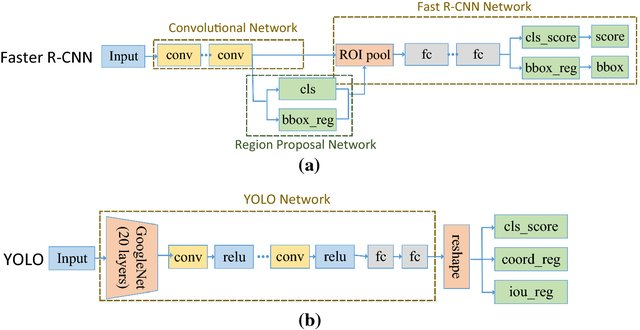
\includegraphics[width=0.95\linewidth]{figures/fastrcnn_vs_yolo}
        \caption{(a) A two-stage Faster R-CNN object detector. (b) A one-stage YOLO object detector. Figure from Li et al. (2019) \cite{liEnhancedBirdDetection2019}.
        % The two-stage detector requires two forward passes through the network, while the one-stage detector only requires one. 
        }
        \label{fig:fastrcnn_vs_yolo}
    \end{figure}

    The SOTA status of two-stage object detection methods precedes that of their one-stage counterpart. The popularity of CNNs in the CV field in the early 2010s led to the development of \textbf{RCNN} (2014). This architecture first proposes image regions by selective search \cite{uijlingsSelectiveSearchObject2013}, which are then rescaled and fed into a CNN to extract features to finally use a linear classifier to predict their label \cite{girshickRichFeatureHierarchies2014}. 
    
    The success of RCNN for object detection tasks was followed by SPP-Net (2014), which introduced a Spatial Pyramid Pooling (SPP) layer to allow the model to process images of arbitrary sizes without rescaling them \cite{heSpatialPyramidPooling2014}. Then came \textbf{Fast RCNN} and \textbf{Faster R-CNN} in 2015 \cite{girshickFastRCNN2015,renFasterRCNNRealTime2016}, who respectively improved on RCNN by training the detector and bounding box regressor jointly, and by using a Region Proposal Network (RPN) to replace the much slower selective search algorithm used by previous models. 
    
    While two-stage detectors were achieving state-of-the-art performance in terms of accuracy, they were not fast enough to be used for real-time applications or on embedded devices such as smartphones. This led to the need to develop faster object detection methods that could be used for such purposes \cite{zouObjectDetection202023b}.
    
    It wasn't until 2016 that one-stage object detectors reached this milestone with the proposal of the \textbf{YOLO} (You Only Look Once) model \cite{redmonYouOnlyLook2016}. Unlike RCNN-based approaches, YOLO poses the task as a regression problem, where the model directly predicts the bounding boxes and class probabilities of the objects in one evaluation, allowing the system to be optimized in an end-to-end fashion. 
    % This approach allowed YOLO to achieve real-time performance comparable to Faster R-CNN.

     YOLO marked a turning point in the field, a surge in the popularity of one-stage detectors led to more methods being proposed in the following years, from more adequate loss functions like RetinaNet's Focal Loss \cite{linFocalLossDense2018} to subsequent developments to YOLO's architecture like YOLO9K (2016), YOLOv3 (2018), and YOLOv8 (2023) \cite{redmonYOLO9000BetterFaster2016, redmonYOLOv3IncrementalImprovement2018, Jocher_YOLO_by_Ultralytics_2023} that improved on the original model's performance, allowing it to retain SOTA performance.
     
     In this age, single-stage object detectors dominate the general benchmarks (e.g., ISLVR, COCO \cite{linMicrosoftCOCOCommon2015}, PASCAL VOC \cite{everinghamPascalVisualObject2010}) in both accuracy and speed. More recent methods use Transformer architectures \cite{vaswaniAttentionAllYou2017} to overcome the limitations of traditional CNNs in terms of parallelization and locally restrictive receptive field, showing that abandoning convolutions in favor of an attention-only approach can also achieve SOTA \cite{ carionEndtoEndObjectDetection2020,zhuDeformableDETRDeformable2021}.
    
    \subsection{Tuberculosis Detection using Machine Learning Methods} \label{sec:ml_tuberculosis_detection} \todo{1-1.5 pages}

    While general object detection methods have achieved outstanding performance for more common object detection tasks, like detecting cars, people, or animals from images 
    that could be taken in a wide range of conditions (i.e., those that most people would be able to identify), they tend to perform poorly when applied to more domain-specific tasks.
    
    This problem is because models like those described in the previous subsection are trained on big datasets of images that can be commonly found on the internet and are easier to annotate, which tend to exclude more specialized images that are hard to obtain and even harder to annotate.

    Furthermore, two-stage object detections like YOLO tend to perform poorly when applied to images containing small objects (e.g., cells, bacteria, etc.)  because their region proposal mechanism favors larger objects with a clear distinction from the background. 

    These latter issues present a problem with the type of datasets usually available for medical applications, where images are typically taken in a more controlled environment and contain objects that only experts in the specific domain can identify. Furthermore, it is likely for objects of interest in medical images to be small and difficult to distinguish, as the need for specialized devices - often noise-prone and with low spatial resolution - is a common thing in the field.

    This is the case of the kind of dataset used for TB detection, which is of interest in this work. \textbf{In sputum-microscopy images}, for example, the objects of interest are the bacilli that cause tuberculosis, tiny bacteria that are small and challenging to distinguish from other organic materials that surround them \cite{osman_tuberculosis_2011}. This makes the detection of tuberculosis a task that requires more specialized methods to achieve good performance.

    But even though the models that achieve SOTA in general benchmarks tend to fail for medical applications right out of the box, that doesn't mean that they cannot be adapted to more specialized datasets. In fact, the same methods have also been shown to perform well for medical applications when \textbf{adapted} to the task, and TB detection is no exception.

    Some of the earliest examples we can find in the literature of the use of DL methods for detecting TB come from the work of Osman et al. in the 2010s \cite{osmanDetectionMycobacteriumTuberculosis2010,osman_tuberculosis_2011,ahmadGeneticAlgorithmArtificialNeural2010}. Osman studied the use of techniques like multilayer perceptron (MPL) networks, K-Means clustering, and genetic algorithms, combined with more classical CV techniques like color thresholding and morphological operations, to detect and segment TB in \textbf{Ziehl-Neelsen (ZN) stained sputum smear} microscopy images. 

    More recently, Lakhani and Sundaram (2017) \cite{lakhaniDeepLearningChest2017} used CNNs to classify Tuberculosis from chest X-ray images automatically. The authors used a deidentified dataset composed of 1007 posteroanterior chest radiographs, of which 15\% were used for testing. The model achieved an AUC of 0.99 with an ensemble of AlexNet \cite{krizhevskyImageNetClassificationDeep2012} and GoogLeNet \cite{szegedyGoingDeeperConvolutions2014} models.
    
    \begin{figure}[h]
       \centering
       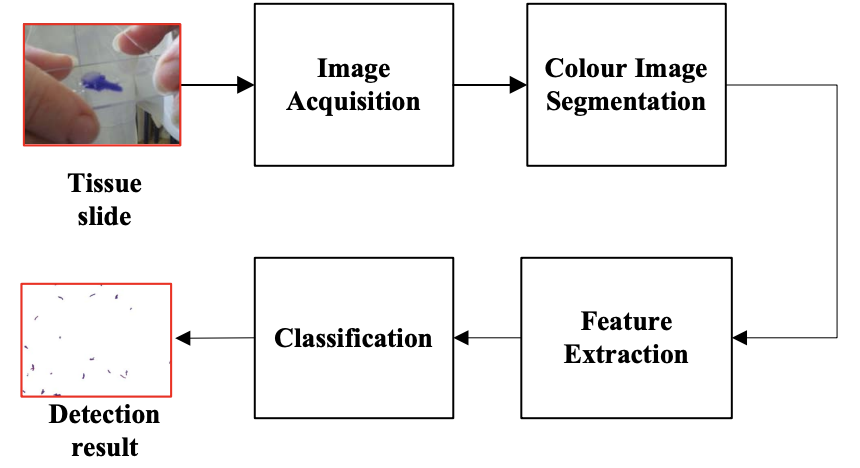
\includegraphics[width=0.8\linewidth]{osman_tb_example}
       \caption{Block diagram of the method proposed by Osman et al. (2010) \cite{osmanDetectionMycobacteriumTuberculosis2010} for automated TB bacilli detection from sputum-smear microscopy images.}
       \label{fig:visuna_method}
    \end{figure}
    \clearpage

    Roy et al. (2020) \cite{royDeepLearningClassification2020} presented a deep learning-based method for the assisted diagnosis of \textbf{COVID-19} markers from lung ultrasonography (LUS) images. The researchers collected data from six Italian hospitals and used it to train a CNN architecture derived from Spatial Transformers \cite{jaderbergSpatialTransformerNetworks2016} (not related to Attention-based Transformers) to classify LUS images as either healthy or pathological and segment the affected area. The model was trained on 77 LUS videos from 35 patients for a total of 58,924 image frames and achieved a semantic segmentation accuracy of 96\%.
    

     The study most close to our work comes from Visuña et al. (2023) \cite{visuna_novel_2023}, which presented a DL-based technique to localize tuberculosis present on sputum smear microscopy images. The author used a \textbf{one-stage object detection method} with a Convolutional Neural Network backbone to detect the presence of bacilli in the images. 
     
     Visuña first fragmented the image into patches of 80x80 pixels and then \textbf{classified each patch as either containing bacilli or not} for maximum spatial coverage. This study is very relevant to our use case since it uses the same dataset that we will study in this work. Her model was trained on 200 microscopy stain images and, using a 70/30 train/test split, achieved a 99.49\% % precision and 92.86\% % recall on the test set. 

    
    \subsection{Continually Adaptive Systems} \label{sec:continually_adaptive_systems_sota} 
    % \todo{0.5 pages}

    Continually adaptive systems are systems that can adapt to changes in their environment instantly or over time. They are often used in applications where the environment is constantly changing, such as in robotics or autonomous vehicles. The thesis of this work is about considering their use case in a healthcare setting. 

    Casimiro et al. (2022) discusses the challenges and opportunities of self-adaptive systems (SAS) in machine learning. The authors propose a framework for the development of SAS that rely on ML components. This framework is based on the concept of \textbf{MAPE-K} loops \cite{kephartVisionAutonomicComputing2003}, which consists of a set of modules that allow the system to \textbf{M}onitor, \textbf{A}nalyze, \textbf{P}lan, and \textbf{E}xecute changes to itself (\textit{tactics}) with the help of a \textbf{K}nowledge base that tracks the system's behavior (see figure \ref{fig:mape-k}).

    \begin{figure}[h]
        \centering
        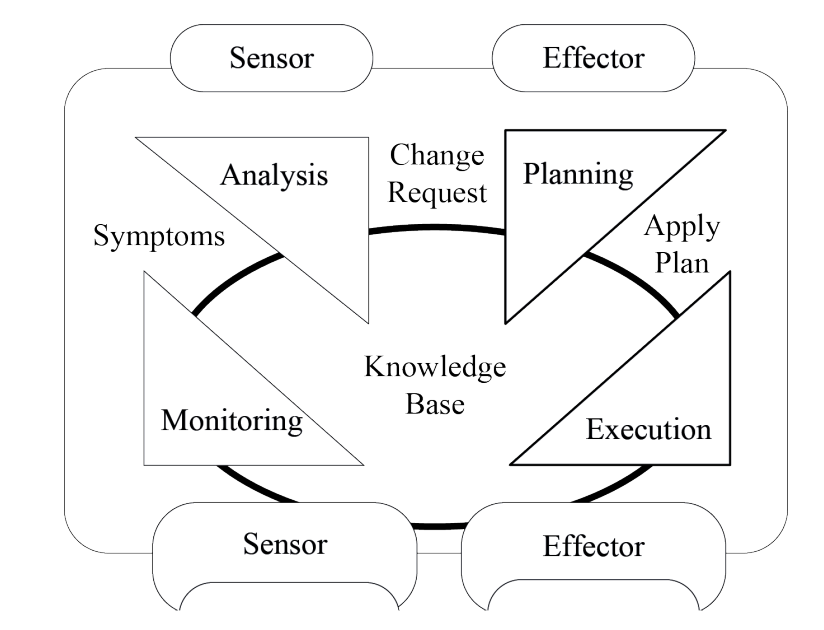
\includegraphics[width=0.48\textwidth]{mape_k_loop.png}
        \caption{The original MAPE-K Loop, as first introduced by IBM in 2004. Source: \cite{redbooks_practical_2004}}
        \label{fig:mape-k}
    \end{figure}
    
    The authors discuss the required changes to the traditional MAPE-K loop and the challenges associated with developing such systems for ML applications. They motivate their ideas by presenting a case study of SAS in the enterprise (ES) and cyber-physical (CPS) system domains. Table \ref{tab:casimiro_problems} shows an example of the problems they identified in these domains along with the learning-based tactics considered to solve them.
    
    Note how rather than focusing on how to obtain a plan to adapt the system, Casimiro et al.'s approach is to identify first the specific \textbf{causes of degradation} within each domain to then characterize the appropriate \textbf{adaptation tactics}. 

    Similar works such as Gheibi et al. (2020) \cite{gheibiApplyingMachineLearning2020}, which makes a review of the literature on machine learning applied to self-adaptive systems, also focuses on the use of MAPE-K loops to develop such systems. However, the scope of the study is about using ML to support SAS rather than using the latter to support the learning process.
    
    Note that the difference between the two approaches is subtle but important. In the first case, the problem is about using learning algorithms as a means to support the adaptive system without considering the tasks that it executes. The task of the ML model, then, is to improve one or more functions of the MAPE loop. For example, to predict the best tactic to use in a given situation (Planning) or detecting anomalies in the behavior of the system (Monitoring).

    In the second case, the one we care about, the problem is about using the MAPE-K loop as a means to \textbf{improve the learning process} of an ML model. That is, we are putting the learning process at the center of the system, and the task of the MAPE-K loop is to support it with any tactic (learning-based or not) that can help improve the performance and/or efficiency of the model. 

    % In the first case, the problem is about using ML to improve the adaptation process of the system, for example, to 

    % That study is very relevant to the work in this thesis since the approach we take is very similar to theirs. Although we consider a larger set of tactics that can be used to adapt the system and apply it to the problem of object detection in medical images.
    

    \begin{table}
        \resizebox*{0.95\columnwidth}{!}{
            \begin{tabular}{l | l l l}
            \toprule
            \textbf{Problem} & \textbf{Domain} & \textbf{Example Situation} & \textbf{Applicable Tactics} \\ 
            \midrule
            \multirow{4}{*}{Covariate shift} & ES & Transaction patterns change & \(\bullet\) Component replacement \\  
            & & Adversaries poison data & \(\bullet\) Unlearning \\ \cline{2-4}  & & Noise/uncertainty in sensors & \(\bullet\) Transfer learning \\ 
            \cline{3-4}  & \multirow{2}{*}{CPS} & Different lighting conditions & \(\bullet\) Component replacement \\  
            & & for face recognition &  \\ 
            \cline{3-4}  & & Adversaries manipulate smart meter data & \(\bullet\) Human-based labeling \\ 
            & & & \(\bullet\) Unlearning \\
            \hline \multirow{2}{*}{Label shift} & ES & Variable fraud rate & \(\bullet\) Human-based labeling \\ 
            \cline{2-4}  & CPS & Unknown command for voice controller & \(\bullet\) Human-based labeling \\ 
            \hline \multirow{2}{*}{Concept shift} & ES & New fraud strategies & \(\bullet\) Transfer learning \\ 
            \cline{2-4}  & CPS & Inhabitant’s living patterns & \(\bullet\) Retrain \\ 
            & & & \(\bullet\) Unlearning \\
            \bottomrule
            \end{tabular}
        }
        \caption{Casimiro et al. (2022) \cite{casimiro_self-adaptive_2022}: Example of problems of Learning Systems within each domain and tactics to solve them.}
        \label{tab:casimiro_problems}
        \vspace*{-0.4cm}
    \end{table}
    
    The idea of bringing MAPE-K loops to the context of this work is that much like traditional software systems, ML can also benefit from the study of SAS techniques (and the ample literature that exists on the topic) to improve their performance and robustness.
    % Indeed, the idea of continual adaptation is not new to the ML field, with well-known researchers arguing that it is a fundamental aspect of intelligence \cite{kirsch_self-referential_2022,thrun_lifelong_1995, parisi_continual_2019}. 

    In her book `Designing Machine Learning Systems' \cite{huyen_designing_2022}, Chip Huyen presents the challenges and patterns of deploying ML Systems. Like Casimiro et al., she stresses the importance of monitoring a model's behavior to identify causes of degradation and continually update them. She also discusses how having humans in the loop who can provide feedback to the system is essential for their reliability in high-stakes domains.

    Vokinger et al. (2021) makes further discussion about the reliability of continually-adapted systems in healthcare, arguing that the risk that such systems pose in such a domain is likely the reason why the FDA has not approved any continual-learning systems for medical use \cite{vokingerContinualLearningMedical2021}. The authors highlight problems like \textbf{catastrophic forgetting} and \textbf{bias induction} as two inherent risks of continual learning systems to address.

    Adaptive systems that have been deployed for health uses can be more commonly found in the remote sensing domain, where typically a set of sensors is used to monitor signals from the user's body to obtain fitness-related insights. Jha et al. (2021) \cite{jhaContinualLearningSensorbased2021}, for example, makes an empirical analysis of continual learning applied to Human-Activity Recognition models that can learn to recognize new activities over time different from the ones they were initially trained on.
    
    A different approach to self-adaptivity comes from the authors of MsO-KELM \cite{haoTechnologyOrientedPathwayAuxiliary2022}, a system that takes a kernel extreme learning machine (KELM) model \cite{xiaEvolvingKernelExtreme2022} and introduces a swarm intelligence algorithm to optimize its hyperparameters in a self-adaptive manner. The authors show that their system can achieve better performance than other KELM-based models. This approach, however, suffers from the lack of flexibility MAPE-K loops provide, as it is not clear how this system would adapt to other problems or models.
    
    In the next section, we will characterize some adaptation techniques and learning paradigms proposed in the literature that could be used as \textit{tactics} of a continual-learning system that tackles the problems described in this work.
    
    
    % ConvLSTM, Graph Neural Networks
    \section{Adaptation Techniques and Learning Paradigms} \label{sec:relevant_techniques} 
    % \info{6-7 pages}

    Throughout this section, we consider a set of novel techniques proposed in the literature related to ML model adaptation. One of the critical aspects in selecting which methods to include in this section - besides their relevance to the topic - was the technical feasibility of implementing them as \textit{tactics} (as described above) in a self-adaptive system. 

    The idea is that some of the techniques described here may be used as the basis for the adaptation process of an ML model after it has been detected (through specific monitorization) that some form of degradation has occurred. The goal would be to then use some of these techniques (or a combination of them) as a way to improve performance.

    \subsection{Continual Learning} \label{sec:continual_learning} 
    % \info{1.25 pages}
	
    Continual learning refers to the concept of constantly updating a model as new information arrives, allowing it to adapt to changing data \cite{huyen_designing_2022}. This is, of course, at the core of the problem we are trying to solve in this work. Rather than a specific method or technique, continual learning is a framework that encompasses a set of techniques that allow an ML system to learn continually from a data stream.

    In its most basic form,  continual learning is about updating the model when new data becomes available. However, this is not as simple as it sounds. The key to a successful continual learning process is that the model is updated such that it performs well on the new data without hurting it in the task it was designed for. While obvious, this is not a trivial problem, and it is a particularly known weak point of current ML algorithms. Often called the \textbf{stability-plasticity dilemma} \cite{mermillodStabilityplasticityDilemmaInvestigating2013}.

    Richard Sutton, one of the pioneers of the field of reinforcement learning (and author of the infamous article `\href{https://www.cs.utexas.edu/~eunsol/courses/data/bitter_lesson.pdf}{The Bitter Lesson}' \cite{suttonBitterLesson2019}), has very recently studied this problem in \textit{deep supervised learning models}, a subject that is very relevant to this work. In an August 2023 paper (and seminar), he makes the big claim that `Deep learning does not work for continual learning' \cite{dohareLossPlasticityDeep2023}. 
    
    This statement is a bit exaggerated (by Sutton's own admission). What he argues about really is the reality that DNNs tend to eventually become very slow to learn from new data, eventually leading to a catastrophic loss of performance. This phenomenon is denominated \textbf{loss of plasticity}.

    Problems with DNN plasticity have been studied before, Ash et. al's (2019) \cite{ashWarmStartingNeuralNetwork2020} was a very influential paper that discussed the failure of warm-starting neural networks, and proposed a regularization method consisting of shrinking and perturbing slightly the weights of the network at every optimization step, which improved significantly the performance of continual learning tasks.

    Related to plasticity is \textbf{catastrophic forgetting}, when models forget previously learned information when trained on new data, which is another well-studied problem with ML algorithms \cite{mccloskeyCatastrophicInterferenceConnectionist1989,huyen_designing_2022,parisiContinualLifelongLearning2019}. Beyond that, there are other myriads of issues to face when implementing a continual learning setting: how to select the optimal samples to train the model with, dealing with class imbalance, improving hardware efficiency, how to store and manage the data and evaluate performance, to name a few.

     Adding more to their complexity, we can consider two frameworks for implementing continual learning in a machine-learning system: \textit{offline} and \textit{online} continual learning. 
    
    Learning offline is the most typical example where the model is updated periodically using a batch of data obtained over time, i.e., the model is updated only when a certain amount of \textit{new} data has been collected (and labeled, in the supervised case). This is the most common approach in the literature and also the easiest to implement.
    
    % Offline learning can be additionally subdivided into two categories based on how data is monitored before updating a model: \textit{passive} and \textit{active} continual learning.

    % The model is updated passively when the data is collected over a fixed period of time (e.g., every six months) or after a fixed number of instances have been processed and labeled (e.g., every 1000 new instances). Conversely, the model is updated actively when we update only when the model's performance drops below a certain threshold or when the system detects a significant change in the data distribution \cite{huyen_designing_2022}.

   Online learning is the second framework. In this case, the model is adapted as soon as new data arrives, with every new instance - or very small batch of instances - being used to update it. This approach is optimal when it is adamant for the model to adapt to the data as soon as it arrives (streaming applications, for example). 
   
   However, online learning algorithms tend to be more computationally expensive than offline learning and can be less effective than their offline counterparts, they are also likely to suffer even more from catastrophic forgetting \cite{huyen_designing_2022}.

   The work in this thesis is all about adopting continual learning for healthcare applications. It is not only suitable in applications where data arrives in a stream (e.g., wearable health monitors) but also in cases where the data is collected periodically (e.g., medical imaging). In both cases, the data is likely to change over time, and the model needs to adapt to it. We'll continue this section with techniques that can be used to implement or improve a continual learning system and face the challenges described above.

    \subsection{Transfer Learning and Domain Adaptation} \label{sec:transfer_learning} 
    % \info{1 page}

    Transfer learning is a technique that aims to improve the performance of a model by `transferring' the knowledge of a pre-trained model to a new task. This is achieved by first training the model on a large dataset - that was presumably easy to obtain - from which it can learn general features and patterns of the data modality, and then \textbf{fine-tuning} it on a smaller dataset specific to the new task. Avoiding the need to train the model from scratch on the new dataset allows the model to achieve better performance with less data and training time \cite{panSurveyTransferLearning2010}.

     Nowadays transfer learning has been adopted widely by the Deep Learning community in parts because it allows researchers and practitioners in the industry alike to effectively `recycle' models that have been trained and shared previously on large datasets and apply them for their own purposes. Thus saving the - often prohibitively - expensive time and resources required to train deep-learning models from scratch on such significant amounts of data  \cite{yosinskiHowTransferableAre2014}.

     Furthermore, it has been shown that initializing a neural network with pre-trained weights (i.e., using transfer learning) can help the model converge faster and achieve better generalization than training it from scratch. Showing the model can leverage the knowledge learned from previous data to learn the new task more efficiently \cite{yosinskiHowTransferableAre2014}.

     Transfer Learning is useful for healthcare applications because it allows us to adapt pre-trained models to the medical domain - something referred to as \textbf{domain adaptation}. This is particularly relevant to our problem, we can use transfer learning to adapt models trained on general object detection datasets (e.g., COCO \cite{linMicrosoftCOCOCommon2015}, PASCAL VOC \cite{everinghamPascalVisualObject2010}) to the task of detecting tuberculosis in microscopy images. Something that has been done before in the literature with good results \cite{visuna_novel_2023}.

     \clearpage

     We can envision this technique as part of a continual system that automatically adapts machine learning components to new tasks using transfer learning, avoiding the need to retrain the entire model from scratch.

    % \clearpage
	
    \subsection{Active Learning} \label{sec:active_learning} 
    % \info{1.25 pages}
 
     Active learning strategies selectively acquire data based on their informativeness or uncertainty to the model. Its value comes from allowing the model to guide its own data acquisition process, thus potentially reducing the need for vast - or unnecessary - amounts of pre-labeled data before a model is trained or updated \cite{huyen_designing_2022, chen_study_2015, figueroa_predicting_2012}. 
    %  This is particularly important in health applications, as the availability of annotated medical data is often limited due to privacy concerns, expert time constraints, and the complexity of pathological findings.
     
     Active learning enables the development of accurate models using significantly less labeled data, paving the way for more efficient and cost-effective healthcare systems. 
     
     Some common active learning strategies include uncertainty sampling, query by committee, and expected model change. 

     \newpage

    \begin{figure}
        \centering
        \caption{Illustrations of the relevant Machine Learning Paradigms and Techniques}
        \resizebox*{1.15\columnwidth}{!}{
            \hspace*{-1.5cm}
            

\tikzset{every picture/.style={line width=0.75pt}} %set default line width to 0.75pt        

\begin{tikzpicture}[x=0.75pt,y=0.75pt,yscale=-1,xscale=1]
%uncomment if require: \path (0,1369); %set diagram left start at 0, and has height of 1369

%Rounded Rect [id:dp7169655314014065] 
\draw  [fill={rgb, 255:red, 184; green, 233; blue, 134 }  ,fill opacity=0.57 ][dash pattern={on 4.5pt off 4.5pt}] (656.53,1123.76) .. controls (656.53,1104.67) and (672.01,1089.2) .. (691.09,1089.2) -- (998.97,1089.2) .. controls (1018.06,1089.2) and (1033.53,1104.67) .. (1033.53,1123.76) -- (1033.53,1227.44) .. controls (1033.53,1246.53) and (1018.06,1262) .. (998.97,1262) -- (691.09,1262) .. controls (672.01,1262) and (656.53,1246.53) .. (656.53,1227.44) -- cycle ;
%Shape: Ellipse [id:dp3446272829293622] 
\draw  [fill={rgb, 255:red, 245; green, 166; blue, 35 }  ,fill opacity=1 ][line width=0.75]  (803.27,1125.05) .. controls (803.27,1114.95) and (810.71,1106.76) .. (819.88,1106.76) .. controls (829.06,1106.76) and (836.5,1114.95) .. (836.5,1125.05) .. controls (836.5,1135.15) and (829.06,1143.33) .. (819.88,1143.33) .. controls (810.71,1143.33) and (803.27,1135.15) .. (803.27,1125.05) -- cycle ;
%Straight Lines [id:da791317241793424] 
\draw [line width=0.75]    (721.98,1124.66) -- (742.48,1125.08) ;
\draw [shift={(744.48,1125.12)}, rotate = 181.16] [color={rgb, 255:red, 0; green, 0; blue, 0 }  ][line width=0.75]    (10.93,-3.29) .. controls (6.95,-1.4) and (3.31,-0.3) .. (0,0) .. controls (3.31,0.3) and (6.95,1.4) .. (10.93,3.29)   ;
%Shape: Ellipse [id:dp931419430699773] 
\draw  [fill={rgb, 255:red, 245; green, 166; blue, 35 }  ,fill opacity=1 ][line width=0.75]  (744.48,1125.12) .. controls (744.48,1115.34) and (751.68,1107.41) .. (760.57,1107.41) .. controls (769.46,1107.41) and (776.66,1115.34) .. (776.66,1125.12) .. controls (776.66,1134.89) and (769.46,1142.82) .. (760.57,1142.82) .. controls (751.68,1142.82) and (744.48,1134.89) .. (744.48,1125.12) -- cycle ;
%Shape: Ellipse [id:dp6170909074644266] 
\draw  [fill={rgb, 255:red, 245; green, 166; blue, 35 }  ,fill opacity=1 ][line width=0.75]  (862.53,1124.6) .. controls (862.53,1114.5) and (869.97,1106.32) .. (879.15,1106.32) .. controls (888.33,1106.32) and (895.77,1114.5) .. (895.77,1124.6) .. controls (895.77,1134.7) and (888.33,1142.88) .. (879.15,1142.88) .. controls (869.97,1142.88) and (862.53,1134.7) .. (862.53,1124.6) -- cycle ;
%Straight Lines [id:da9337188734209669] 
\draw [fill={rgb, 255:red, 245; green, 166; blue, 35 }  ,fill opacity=1 ][line width=0.75]    (776.66,1125.12) -- (800.53,1124.66) ;
\draw [shift={(803.53,1124.6)}, rotate = 178.9] [fill={rgb, 255:red, 0; green, 0; blue, 0 }  ][line width=0.08]  [draw opacity=0] (8.93,-4.29) -- (0,0) -- (8.93,4.29) -- cycle    ;
%Straight Lines [id:da6741481862943082] 
\draw [fill={rgb, 255:red, 245; green, 166; blue, 35 }  ,fill opacity=1 ][line width=0.75]    (836.5,1125.05) -- (856.53,1125.08) -- (859.54,1124.84) ;
\draw [shift={(862.53,1124.6)}, rotate = 175.41] [fill={rgb, 255:red, 0; green, 0; blue, 0 }  ][line width=0.08]  [draw opacity=0] (8.93,-4.29) -- (0,0) -- (8.93,4.29) -- cycle    ;
%Straight Lines [id:da5385449874502153] 
\draw [line width=0.75]    (954.77,1124.6) -- (979.29,1124.86) ;
\draw [shift={(981.29,1124.88)}, rotate = 180.61] [color={rgb, 255:red, 0; green, 0; blue, 0 }  ][line width=0.75]    (10.93,-3.29) .. controls (6.95,-1.4) and (3.31,-0.3) .. (0,0) .. controls (3.31,0.3) and (6.95,1.4) .. (10.93,3.29)   ;
%Shape: Grid [id:dp8873702019342256] 
\draw  [draw opacity=0] (719.93,1204.6) -- (880.5,1204.6) -- (880.19,1245.2) -- (719.62,1245.2) -- cycle ; \draw   (719.93,1204.6) -- (719.62,1245.2)(739.93,1204.6) -- (739.62,1245.2)(759.93,1204.6) -- (759.62,1245.2)(779.93,1204.6) -- (779.62,1245.2)(799.93,1204.6) -- (799.62,1245.2)(819.93,1204.6) -- (819.62,1245.2)(839.93,1204.6) -- (839.62,1245.2)(859.93,1204.6) -- (859.62,1245.2)(879.93,1204.6) -- (879.62,1245.2) ; \draw   (719.93,1204.6) -- (880.5,1204.6)(719.78,1224.6) -- (880.35,1224.6)(719.63,1244.6) -- (880.19,1244.6) ; \draw    ;
%Shape: Ellipse [id:dp4237537414586634] 
\draw  [fill={rgb, 255:red, 245; green, 166; blue, 35 }  ,fill opacity=1 ][line width=0.75]  (921.53,1124.6) .. controls (921.53,1114.5) and (928.97,1106.32) .. (938.15,1106.32) .. controls (947.33,1106.32) and (954.77,1114.5) .. (954.77,1124.6) .. controls (954.77,1134.7) and (947.33,1142.88) .. (938.15,1142.88) .. controls (928.97,1142.88) and (921.53,1134.7) .. (921.53,1124.6) -- cycle ;
%Straight Lines [id:da9140472890264204] 
\draw [fill={rgb, 255:red, 245; green, 166; blue, 35 }  ,fill opacity=1 ][line width=0.75]    (895.5,1125.05) -- (915.53,1125.08) -- (918.54,1124.84) ;
\draw [shift={(921.53,1124.6)}, rotate = 175.41] [fill={rgb, 255:red, 0; green, 0; blue, 0 }  ][line width=0.08]  [draw opacity=0] (8.93,-4.29) -- (0,0) -- (8.93,4.29) -- cycle    ;
%Shape: Ellipse [id:dp2519862377199167] 
\draw  [fill={rgb, 255:red, 80; green, 227; blue, 194 }  ,fill opacity=1 ][line width=0.75]  (804.27,1176.05) .. controls (804.27,1165.95) and (811.71,1157.76) .. (820.88,1157.76) .. controls (830.06,1157.76) and (837.5,1165.95) .. (837.5,1176.05) .. controls (837.5,1186.15) and (830.06,1194.33) .. (820.88,1194.33) .. controls (811.71,1194.33) and (804.27,1186.15) .. (804.27,1176.05) -- cycle ;
%Straight Lines [id:da47767827809070895] 
\draw [fill={rgb, 255:red, 80; green, 227; blue, 194 }  ,fill opacity=1 ][line width=0.75]    (722.98,1175.66) -- (743.48,1176.08) ;
\draw [shift={(745.48,1176.12)}, rotate = 181.16] [color={rgb, 255:red, 0; green, 0; blue, 0 }  ][line width=0.75]    (10.93,-3.29) .. controls (6.95,-1.4) and (3.31,-0.3) .. (0,0) .. controls (3.31,0.3) and (6.95,1.4) .. (10.93,3.29)   ;
%Shape: Ellipse [id:dp4749788359388263] 
\draw  [fill={rgb, 255:red, 80; green, 227; blue, 194 }  ,fill opacity=1 ][line width=0.75]  (745.48,1176.12) .. controls (745.48,1166.34) and (752.68,1158.41) .. (761.57,1158.41) .. controls (770.46,1158.41) and (777.66,1166.34) .. (777.66,1176.12) .. controls (777.66,1185.89) and (770.46,1193.82) .. (761.57,1193.82) .. controls (752.68,1193.82) and (745.48,1185.89) .. (745.48,1176.12) -- cycle ;
%Shape: Ellipse [id:dp0313589628022779] 
\draw  [fill={rgb, 255:red, 80; green, 227; blue, 194 }  ,fill opacity=1 ][line width=0.75]  (863.53,1175.6) .. controls (863.53,1165.5) and (870.97,1157.32) .. (880.15,1157.32) .. controls (889.33,1157.32) and (896.77,1165.5) .. (896.77,1175.6) .. controls (896.77,1185.7) and (889.33,1193.88) .. (880.15,1193.88) .. controls (870.97,1193.88) and (863.53,1185.7) .. (863.53,1175.6) -- cycle ;
%Straight Lines [id:da020882303258308976] 
\draw [fill={rgb, 255:red, 80; green, 227; blue, 194 }  ,fill opacity=1 ][line width=0.75]    (777.66,1176.12) -- (801.53,1175.66) ;
\draw [shift={(804.53,1175.6)}, rotate = 178.9] [fill={rgb, 255:red, 0; green, 0; blue, 0 }  ][line width=0.08]  [draw opacity=0] (8.93,-4.29) -- (0,0) -- (8.93,4.29) -- cycle    ;
%Straight Lines [id:da6483918021597859] 
\draw [fill={rgb, 255:red, 80; green, 227; blue, 194 }  ,fill opacity=1 ][line width=0.75]    (837.5,1176.05) -- (857.53,1176.08) -- (860.54,1175.84) ;
\draw [shift={(863.53,1175.6)}, rotate = 175.41] [fill={rgb, 255:red, 0; green, 0; blue, 0 }  ][line width=0.08]  [draw opacity=0] (8.93,-4.29) -- (0,0) -- (8.93,4.29) -- cycle    ;
%Straight Lines [id:da8962594595879614] 
\draw [fill={rgb, 255:red, 80; green, 227; blue, 194 }  ,fill opacity=1 ][line width=0.75]    (955.77,1175.6) -- (980.29,1175.86) ;
\draw [shift={(982.29,1175.88)}, rotate = 180.61] [color={rgb, 255:red, 0; green, 0; blue, 0 }  ][line width=0.75]    (10.93,-3.29) .. controls (6.95,-1.4) and (3.31,-0.3) .. (0,0) .. controls (3.31,0.3) and (6.95,1.4) .. (10.93,3.29)   ;
%Shape: Ellipse [id:dp1806728163736684] 
\draw  [fill={rgb, 255:red, 80; green, 227; blue, 194 }  ,fill opacity=1 ][line width=0.75]  (922.53,1175.6) .. controls (922.53,1165.5) and (929.97,1157.32) .. (939.15,1157.32) .. controls (948.33,1157.32) and (955.77,1165.5) .. (955.77,1175.6) .. controls (955.77,1185.7) and (948.33,1193.88) .. (939.15,1193.88) .. controls (929.97,1193.88) and (922.53,1185.7) .. (922.53,1175.6) -- cycle ;
%Straight Lines [id:da7007331216346642] 
\draw [fill={rgb, 255:red, 80; green, 227; blue, 194 }  ,fill opacity=1 ][line width=0.75]    (896.5,1176.05) -- (916.53,1176.08) -- (919.54,1175.84) ;
\draw [shift={(922.53,1175.6)}, rotate = 175.41] [fill={rgb, 255:red, 0; green, 0; blue, 0 }  ][line width=0.08]  [draw opacity=0] (8.93,-4.29) -- (0,0) -- (8.93,4.29) -- cycle    ;
%Curve Left Arrow [id:dp11887902175153586] 
\draw  [fill={rgb, 255:red, 248; green, 118; blue, 109 }  ,fill opacity=1 ] (661.53,1148.1) .. controls (661.53,1134.02) and (678.46,1122.6) .. (699.33,1122.6) -- (699.33,1129.6) .. controls (678.46,1129.6) and (661.53,1141.02) .. (661.53,1155.1) ;\draw  [fill={rgb, 255:red, 248; green, 118; blue, 109 }  ,fill opacity=1 ] (661.53,1155.1) .. controls (661.53,1166.4) and (672.44,1175.99) .. (687.53,1179.33) -- (687.53,1186.33) -- (699.33,1177.1) -- (687.53,1165.33) -- (687.53,1172.33) .. controls (672.44,1168.99) and (661.53,1159.4) .. (661.53,1148.1)(661.53,1155.1) -- (661.53,1148.1) ;

%Rounded Rect [id:dp6082348604231713] 
\draw  [fill={rgb, 255:red, 80; green, 227; blue, 194 }  ,fill opacity=0.55 ][dash pattern={on 4.5pt off 4.5pt}] (832.88,881.38) .. controls (832.88,864.82) and (846.31,851.4) .. (862.86,851.4) -- (998.02,851.4) .. controls (1014.58,851.4) and (1028,864.82) .. (1028,881.38) -- (1028,971.32) .. controls (1028,987.88) and (1014.58,1001.3) .. (998.02,1001.3) -- (862.86,1001.3) .. controls (846.31,1001.3) and (832.88,987.88) .. (832.88,971.32) -- cycle ;
%Rounded Rect [id:dp26696304336209087] 
\draw  [fill={rgb, 255:red, 208; green, 2; blue, 27 }  ,fill opacity=0.45 ][dash pattern={on 4.5pt off 4.5pt}] (590.2,884.05) .. controls (590.2,867.99) and (603.22,854.97) .. (619.28,854.97) -- (757.92,854.97) .. controls (773.98,854.97) and (787,867.99) .. (787,884.05) -- (787,971.28) .. controls (787,987.34) and (773.98,1000.36) .. (757.92,1000.36) -- (619.28,1000.36) .. controls (603.22,1000.36) and (590.2,987.34) .. (590.2,971.28) -- cycle ;
%Shape: Ellipse [id:dp8252888976798756] 
\draw  [color={rgb, 255:red, 74; green, 74; blue, 74 }  ,draw opacity=1 ][fill={rgb, 255:red, 245; green, 166; blue, 35 }  ,fill opacity=1 ][line width=0.75]  (699.06,887.75) .. controls (699.06,881.2) and (704.25,875.88) .. (710.65,875.88) .. controls (717.05,875.88) and (722.23,881.2) .. (722.23,887.75) .. controls (722.23,894.3) and (717.05,899.62) .. (710.65,899.62) .. controls (704.25,899.62) and (699.06,894.3) .. (699.06,887.75) -- cycle ;
%Shape: Ellipse [id:dp946772384134347] 
\draw  [color={rgb, 255:red, 74; green, 74; blue, 74 }  ,draw opacity=1 ][fill={rgb, 255:red, 245; green, 166; blue, 35 }  ,fill opacity=1 ][line width=0.75]  (699.06,921.67) .. controls (699.06,915.12) and (704.25,909.81) .. (710.65,909.81) .. controls (717.05,909.81) and (722.23,915.12) .. (722.23,921.67) .. controls (722.23,928.23) and (717.05,933.54) .. (710.65,933.54) .. controls (704.25,933.54) and (699.06,928.23) .. (699.06,921.67) -- cycle ;
%Shape: Ellipse [id:dp21198631420908698] 
\draw  [color={rgb, 255:red, 74; green, 74; blue, 74 }  ,draw opacity=1 ][fill={rgb, 255:red, 245; green, 166; blue, 35 }  ,fill opacity=1 ][line width=0.75]  (699.68,955.88) .. controls (699.68,949.67) and (704.59,944.65) .. (710.65,944.65) .. controls (716.7,944.65) and (721.61,949.67) .. (721.61,955.88) .. controls (721.61,962.08) and (716.7,967.11) .. (710.65,967.11) .. controls (704.59,967.11) and (699.68,962.08) .. (699.68,955.88) -- cycle ;
%Straight Lines [id:da21282266936209027] 
\draw [color={rgb, 255:red, 74; green, 74; blue, 74 }  ,draw opacity=1 ][fill={rgb, 255:red, 245; green, 166; blue, 35 }  ,fill opacity=1 ][line width=0.75]    (596.65,872.7) -- (618.72,873.07) ;
\draw [shift={(620.72,873.11)}, rotate = 180.97] [color={rgb, 255:red, 74; green, 74; blue, 74 }  ,draw opacity=1 ][line width=0.75]    (10.93,-3.29) .. controls (6.95,-1.4) and (3.31,-0.3) .. (0,0) .. controls (3.31,0.3) and (6.95,1.4) .. (10.93,3.29)   ;
%Shape: Ellipse [id:dp9820468404074927] 
\draw  [color={rgb, 255:red, 74; green, 74; blue, 74 }  ,draw opacity=1 ][fill={rgb, 255:red, 245; green, 166; blue, 35 }  ,fill opacity=1 ][line width=0.75]  (620.72,873.11) .. controls (620.72,866.76) and (625.74,861.61) .. (631.94,861.61) .. controls (638.14,861.61) and (643.17,866.76) .. (643.17,873.11) .. controls (643.17,879.45) and (638.14,884.6) .. (631.94,884.6) .. controls (625.74,884.6) and (620.72,879.45) .. (620.72,873.11) -- cycle ;
%Shape: Ellipse [id:dp9120315482839552] 
\draw  [color={rgb, 255:red, 74; green, 74; blue, 74 }  ,draw opacity=1 ][fill={rgb, 255:red, 245; green, 166; blue, 35 }  ,fill opacity=1 ][line width=0.75]  (620.72,905.76) .. controls (620.72,899.2) and (625.91,893.89) .. (632.31,893.89) .. controls (638.71,893.89) and (643.9,899.2) .. (643.9,905.76) .. controls (643.9,912.31) and (638.71,917.62) .. (632.31,917.62) .. controls (625.91,917.62) and (620.72,912.31) .. (620.72,905.76) -- cycle ;
%Shape: Ellipse [id:dp05281104128609604] 
\draw  [color={rgb, 255:red, 74; green, 74; blue, 74 }  ,draw opacity=1 ][fill={rgb, 255:red, 245; green, 166; blue, 35 }  ,fill opacity=1 ][line width=0.75]  (620.72,936.78) .. controls (620.72,930.57) and (625.63,925.54) .. (631.69,925.54) .. controls (637.74,925.54) and (642.65,930.57) .. (642.65,936.78) .. controls (642.65,942.98) and (637.74,948.01) .. (631.69,948.01) .. controls (625.63,948.01) and (620.72,942.98) .. (620.72,936.78) -- cycle ;
%Shape: Ellipse [id:dp7809611722232168] 
\draw  [color={rgb, 255:red, 74; green, 74; blue, 74 }  ,draw opacity=1 ][fill={rgb, 255:red, 245; green, 166; blue, 35 }  ,fill opacity=1 ][line width=0.75]  (620.1,969.25) .. controls (620.1,962.69) and (625.29,957.38) .. (631.69,957.38) .. controls (638.09,957.38) and (643.28,962.69) .. (643.28,969.25) .. controls (643.28,975.8) and (638.09,981.11) .. (631.69,981.11) .. controls (625.29,981.11) and (620.1,975.8) .. (620.1,969.25) -- cycle ;
%Shape: Ellipse [id:dp7140893324522004] 
\draw  [color={rgb, 255:red, 74; green, 74; blue, 74 }  ,draw opacity=1 ][fill={rgb, 255:red, 245; green, 166; blue, 35 }  ,fill opacity=1 ][line width=0.75]  (756.06,922.11) .. controls (756.06,915.55) and (761.25,910.24) .. (767.65,910.24) .. controls (774.05,910.24) and (779.23,915.55) .. (779.23,922.11) .. controls (779.23,928.66) and (774.05,933.97) .. (767.65,933.97) .. controls (761.25,933.97) and (756.06,928.66) .. (756.06,922.11) -- cycle ;
%Straight Lines [id:da10322635402314129] 
\draw [color={rgb, 255:red, 74; green, 74; blue, 74 }  ,draw opacity=1 ][fill={rgb, 255:red, 245; green, 166; blue, 35 }  ,fill opacity=1 ][line width=0.75]    (643.17,873.11) -- (698.14,883.78) ;
\draw [shift={(700.1,884.16)}, rotate = 190.99] [color={rgb, 255:red, 74; green, 74; blue, 74 }  ,draw opacity=1 ][line width=0.75]    (10.93,-3.29) .. controls (6.95,-1.4) and (3.31,-0.3) .. (0,0) .. controls (3.31,0.3) and (6.95,1.4) .. (10.93,3.29)   ;
%Straight Lines [id:da5069577905309055] 
\draw [color={rgb, 255:red, 74; green, 74; blue, 74 }  ,draw opacity=1 ][fill={rgb, 255:red, 245; green, 166; blue, 35 }  ,fill opacity=1 ][line width=0.75]    (596.65,905.35) -- (618.72,905.72) ;
\draw [shift={(620.72,905.76)}, rotate = 180.97] [color={rgb, 255:red, 74; green, 74; blue, 74 }  ,draw opacity=1 ][line width=0.75]    (10.93,-3.29) .. controls (6.95,-1.4) and (3.31,-0.3) .. (0,0) .. controls (3.31,0.3) and (6.95,1.4) .. (10.93,3.29)   ;
%Straight Lines [id:da7126099084400801] 
\draw [color={rgb, 255:red, 74; green, 74; blue, 74 }  ,draw opacity=1 ][fill={rgb, 255:red, 245; green, 166; blue, 35 }  ,fill opacity=1 ][line width=0.75]    (596.65,936.37) -- (618.72,936.74) ;
\draw [shift={(620.72,936.78)}, rotate = 180.97] [color={rgb, 255:red, 74; green, 74; blue, 74 }  ,draw opacity=1 ][line width=0.75]    (10.93,-3.29) .. controls (6.95,-1.4) and (3.31,-0.3) .. (0,0) .. controls (3.31,0.3) and (6.95,1.4) .. (10.93,3.29)   ;
%Straight Lines [id:da8236884947241534] 
\draw [color={rgb, 255:red, 74; green, 74; blue, 74 }  ,draw opacity=1 ][fill={rgb, 255:red, 245; green, 166; blue, 35 }  ,fill opacity=1 ][line width=0.75]    (643.17,873.11) -- (698.52,916.04) ;
\draw [shift={(700.1,917.27)}, rotate = 217.8] [color={rgb, 255:red, 74; green, 74; blue, 74 }  ,draw opacity=1 ][line width=0.75]    (10.93,-3.29) .. controls (6.95,-1.4) and (3.31,-0.3) .. (0,0) .. controls (3.31,0.3) and (6.95,1.4) .. (10.93,3.29)   ;
%Straight Lines [id:da36577871119376604] 
\draw [color={rgb, 255:red, 208; green, 2; blue, 27 }  ,draw opacity=1 ][fill={rgb, 255:red, 245; green, 166; blue, 35 }  ,fill opacity=1 ][line width=0.75]  [dash pattern={on 4.5pt off 4.5pt}]  (643.17,873.11) -- (700.14,948.78) ;
\draw [shift={(701.34,950.38)}, rotate = 233.02] [color={rgb, 255:red, 208; green, 2; blue, 27 }  ,draw opacity=1 ][line width=0.75]    (10.93,-3.29) .. controls (6.95,-1.4) and (3.31,-0.3) .. (0,0) .. controls (3.31,0.3) and (6.95,1.4) .. (10.93,3.29)   ;
%Straight Lines [id:da5278337040777501] 
\draw [color={rgb, 255:red, 208; green, 2; blue, 27 }  ,draw opacity=1 ][fill={rgb, 255:red, 245; green, 166; blue, 35 }  ,fill opacity=1 ][line width=0.75]  [dash pattern={on 4.5pt off 4.5pt}]  (643.9,905.76) -- (697.16,888.37) ;
\draw [shift={(699.06,887.75)}, rotate = 161.92] [color={rgb, 255:red, 208; green, 2; blue, 27 }  ,draw opacity=1 ][line width=0.75]    (10.93,-3.29) .. controls (6.95,-1.4) and (3.31,-0.3) .. (0,0) .. controls (3.31,0.3) and (6.95,1.4) .. (10.93,3.29)   ;
%Straight Lines [id:da04144940531057717] 
\draw [color={rgb, 255:red, 74; green, 74; blue, 74 }  ,draw opacity=1 ][fill={rgb, 255:red, 245; green, 166; blue, 35 }  ,fill opacity=1 ][line width=0.75]    (643.9,905.76) -- (697.14,921.12) ;
\draw [shift={(699.06,921.67)}, rotate = 196.1] [color={rgb, 255:red, 74; green, 74; blue, 74 }  ,draw opacity=1 ][line width=0.75]    (10.93,-3.29) .. controls (6.95,-1.4) and (3.31,-0.3) .. (0,0) .. controls (3.31,0.3) and (6.95,1.4) .. (10.93,3.29)   ;
%Straight Lines [id:da21511229624898998] 
\draw [color={rgb, 255:red, 208; green, 2; blue, 27 }  ,draw opacity=1 ][fill={rgb, 255:red, 245; green, 166; blue, 35 }  ,fill opacity=1 ][line width=0.75]  [dash pattern={on 4.5pt off 4.5pt}]  (643.9,905.76) -- (698.19,954.54) ;
\draw [shift={(699.68,955.88)}, rotate = 221.94] [color={rgb, 255:red, 208; green, 2; blue, 27 }  ,draw opacity=1 ][line width=0.75]    (10.93,-3.29) .. controls (6.95,-1.4) and (3.31,-0.3) .. (0,0) .. controls (3.31,0.3) and (6.95,1.4) .. (10.93,3.29)   ;
%Straight Lines [id:da1979332040758237] 
\draw [color={rgb, 255:red, 208; green, 2; blue, 27 }  ,draw opacity=1 ][fill={rgb, 255:red, 245; green, 166; blue, 35 }  ,fill opacity=1 ][line width=0.75]  [dash pattern={on 4.5pt off 4.5pt}]  (642.65,936.78) -- (698.25,959.18) ;
\draw [shift={(700.1,959.93)}, rotate = 201.95] [color={rgb, 255:red, 208; green, 2; blue, 27 }  ,draw opacity=1 ][line width=0.75]    (10.93,-3.29) .. controls (6.95,-1.4) and (3.31,-0.3) .. (0,0) .. controls (3.31,0.3) and (6.95,1.4) .. (10.93,3.29)   ;
%Straight Lines [id:da5299687991324811] 
\draw [color={rgb, 255:red, 208; green, 2; blue, 27 }  ,draw opacity=1 ][fill={rgb, 255:red, 245; green, 166; blue, 35 }  ,fill opacity=1 ][line width=0.75]  [dash pattern={on 4.5pt off 4.5pt}]  (643.28,969.25) -- (699.98,963.32) ;
\draw [shift={(701.97,963.11)}, rotate = 174.03] [color={rgb, 255:red, 208; green, 2; blue, 27 }  ,draw opacity=1 ][line width=0.75]    (10.93,-3.29) .. controls (6.95,-1.4) and (3.31,-0.3) .. (0,0) .. controls (3.31,0.3) and (6.95,1.4) .. (10.93,3.29)   ;
%Straight Lines [id:da6814463266434212] 
\draw [color={rgb, 255:red, 208; green, 2; blue, 27 }  ,draw opacity=1 ][fill={rgb, 255:red, 245; green, 166; blue, 35 }  ,fill opacity=1 ][line width=0.75]  [dash pattern={on 4.5pt off 4.5pt}]  (642.65,936.78) -- (698.14,925.31) ;
\draw [shift={(700.1,924.91)}, rotate = 168.33] [color={rgb, 255:red, 208; green, 2; blue, 27 }  ,draw opacity=1 ][line width=0.75]    (10.93,-3.29) .. controls (6.95,-1.4) and (3.31,-0.3) .. (0,0) .. controls (3.31,0.3) and (6.95,1.4) .. (10.93,3.29)   ;
%Straight Lines [id:da8413816684543465] 
\draw [color={rgb, 255:red, 74; green, 74; blue, 74 }  ,draw opacity=1 ][fill={rgb, 255:red, 245; green, 166; blue, 35 }  ,fill opacity=1 ][line width=0.75]    (643.28,969.25) -- (699.7,929.87) ;
\draw [shift={(701.34,928.73)}, rotate = 145.09] [color={rgb, 255:red, 74; green, 74; blue, 74 }  ,draw opacity=1 ][line width=0.75]    (10.93,-3.29) .. controls (6.95,-1.4) and (3.31,-0.3) .. (0,0) .. controls (3.31,0.3) and (6.95,1.4) .. (10.93,3.29)   ;
%Straight Lines [id:da17766491529758244] 
\draw [color={rgb, 255:red, 74; green, 74; blue, 74 }  ,draw opacity=1 ][fill={rgb, 255:red, 245; green, 166; blue, 35 }  ,fill opacity=1 ][line width=0.75]    (643.28,969.25) -- (700.11,896.56) ;
\draw [shift={(701.34,894.98)}, rotate = 128.02] [color={rgb, 255:red, 74; green, 74; blue, 74 }  ,draw opacity=1 ][line width=0.75]    (10.93,-3.29) .. controls (6.95,-1.4) and (3.31,-0.3) .. (0,0) .. controls (3.31,0.3) and (6.95,1.4) .. (10.93,3.29)   ;
%Straight Lines [id:da1917104474490099] 
\draw [color={rgb, 255:red, 74; green, 74; blue, 74 }  ,draw opacity=1 ][fill={rgb, 255:red, 245; green, 166; blue, 35 }  ,fill opacity=1 ][line width=0.75]    (643.06,936.75) -- (698.54,892.41) ;
\draw [shift={(700.1,891.16)}, rotate = 141.37] [color={rgb, 255:red, 74; green, 74; blue, 74 }  ,draw opacity=1 ][line width=0.75]    (10.93,-3.29) .. controls (6.95,-1.4) and (3.31,-0.3) .. (0,0) .. controls (3.31,0.3) and (6.95,1.4) .. (10.93,3.29)   ;
%Straight Lines [id:da6986697533658794] 
\draw [color={rgb, 255:red, 74; green, 74; blue, 74 }  ,draw opacity=1 ][fill={rgb, 255:red, 245; green, 166; blue, 35 }  ,fill opacity=1 ][line width=0.75]    (722.23,887.75) -- (759.96,911.49) ;
\draw [shift={(761.65,912.56)}, rotate = 212.18] [color={rgb, 255:red, 74; green, 74; blue, 74 }  ,draw opacity=1 ][line width=0.75]    (10.93,-3.29) .. controls (6.95,-1.4) and (3.31,-0.3) .. (0,0) .. controls (3.31,0.3) and (6.95,1.4) .. (10.93,3.29)   ;
%Straight Lines [id:da6024220110702969] 
\draw [color={rgb, 255:red, 74; green, 74; blue, 74 }  ,draw opacity=1 ][fill={rgb, 255:red, 245; green, 166; blue, 35 }  ,fill opacity=1 ][line width=0.75]    (722.23,921.67) -- (754.06,922.08) ;
\draw [shift={(756.06,922.11)}, rotate = 180.74] [color={rgb, 255:red, 74; green, 74; blue, 74 }  ,draw opacity=1 ][line width=0.75]    (10.93,-3.29) .. controls (6.95,-1.4) and (3.31,-0.3) .. (0,0) .. controls (3.31,0.3) and (6.95,1.4) .. (10.93,3.29)   ;
%Straight Lines [id:da02990963277339187] 
\draw [color={rgb, 255:red, 208; green, 2; blue, 27 }  ,draw opacity=1 ][fill={rgb, 255:red, 208; green, 2; blue, 27 }  ,fill opacity=1 ][line width=0.75]  [dash pattern={on 4.5pt off 4.5pt}]  (721.61,955.88) -- (758.74,931.48) ;
\draw [shift={(760.41,930.38)}, rotate = 146.69] [color={rgb, 255:red, 208; green, 2; blue, 27 }  ,draw opacity=1 ][line width=0.75]    (10.93,-3.29) .. controls (6.95,-1.4) and (3.31,-0.3) .. (0,0) .. controls (3.31,0.3) and (6.95,1.4) .. (10.93,3.29)   ;
%Straight Lines [id:da9417007474757957] 
\draw [color={rgb, 255:red, 74; green, 74; blue, 74 }  ,draw opacity=1 ][fill={rgb, 255:red, 245; green, 166; blue, 35 }  ,fill opacity=1 ][line width=0.75]    (596.02,968.84) -- (618.1,969.21) ;
\draw [shift={(620.1,969.25)}, rotate = 180.97] [color={rgb, 255:red, 74; green, 74; blue, 74 }  ,draw opacity=1 ][line width=0.75]    (10.93,-3.29) .. controls (6.95,-1.4) and (3.31,-0.3) .. (0,0) .. controls (3.31,0.3) and (6.95,1.4) .. (10.93,3.29)   ;
%Right Arrow [id:dp5555589760224611] 
\draw  [fill={rgb, 255:red, 248; green, 118; blue, 109 }  ,fill opacity=1 ] (789.2,916.35) -- (821.7,916.35) -- (821.7,911.31) -- (831.91,921.4) -- (821.7,931.5) -- (821.7,926.45) -- (789.2,926.45) -- cycle ;
%Shape: Ellipse [id:dp11474745082245863] 
\draw  [color={rgb, 255:red, 74; green, 74; blue, 74 }  ,draw opacity=1 ][fill={rgb, 255:red, 245; green, 166; blue, 35 }  ,fill opacity=1 ][line width=0.75]  (944.65,884.92) .. controls (944.65,878.37) and (949.84,873.05) .. (956.24,873.05) .. controls (962.64,873.05) and (967.83,878.37) .. (967.83,884.92) .. controls (967.83,891.47) and (962.64,896.79) .. (956.24,896.79) .. controls (949.84,896.79) and (944.65,891.47) .. (944.65,884.92) -- cycle ;
%Shape: Ellipse [id:dp8583391052186402] 
\draw  [color={rgb, 255:red, 74; green, 74; blue, 74 }  ,draw opacity=1 ][fill={rgb, 255:red, 245; green, 166; blue, 35 }  ,fill opacity=1 ][line width=0.75]  (944.65,918.84) .. controls (944.65,912.29) and (949.84,906.98) .. (956.24,906.98) .. controls (962.64,906.98) and (967.83,912.29) .. (967.83,918.84) .. controls (967.83,925.4) and (962.64,930.71) .. (956.24,930.71) .. controls (949.84,930.71) and (944.65,925.4) .. (944.65,918.84) -- cycle ;
%Straight Lines [id:da07613466197272079] 
\draw [color={rgb, 255:red, 74; green, 74; blue, 74 }  ,draw opacity=1 ][fill={rgb, 255:red, 245; green, 166; blue, 35 }  ,fill opacity=1 ][line width=0.75]    (842.24,869.87) -- (864.32,870.24) ;
\draw [shift={(866.32,870.28)}, rotate = 180.97] [color={rgb, 255:red, 74; green, 74; blue, 74 }  ,draw opacity=1 ][line width=0.75]    (10.93,-3.29) .. controls (6.95,-1.4) and (3.31,-0.3) .. (0,0) .. controls (3.31,0.3) and (6.95,1.4) .. (10.93,3.29)   ;
%Shape: Ellipse [id:dp6099572577074919] 
\draw  [color={rgb, 255:red, 74; green, 74; blue, 74 }  ,draw opacity=1 ][fill={rgb, 255:red, 245; green, 166; blue, 35 }  ,fill opacity=1 ][line width=0.75]  (866.32,870.28) .. controls (866.32,863.93) and (871.34,858.78) .. (877.54,858.78) .. controls (883.74,858.78) and (888.76,863.93) .. (888.76,870.28) .. controls (888.76,876.62) and (883.74,881.77) .. (877.54,881.77) .. controls (871.34,881.77) and (866.32,876.62) .. (866.32,870.28) -- cycle ;
%Shape: Ellipse [id:dp9046706449073436] 
\draw  [color={rgb, 255:red, 74; green, 74; blue, 74 }  ,draw opacity=1 ][fill={rgb, 255:red, 245; green, 166; blue, 35 }  ,fill opacity=1 ][line width=0.75]  (866.32,902.93) .. controls (866.32,896.37) and (871.5,891.06) .. (877.9,891.06) .. controls (884.3,891.06) and (889.49,896.37) .. (889.49,902.93) .. controls (889.49,909.48) and (884.3,914.79) .. (877.9,914.79) .. controls (871.5,914.79) and (866.32,909.48) .. (866.32,902.93) -- cycle ;
%Shape: Ellipse [id:dp3663560331186333] 
\draw  [color={rgb, 255:red, 74; green, 74; blue, 74 }  ,draw opacity=1 ][fill={rgb, 255:red, 245; green, 166; blue, 35 }  ,fill opacity=1 ][line width=0.75]  (866.32,933.95) .. controls (866.32,927.74) and (871.23,922.72) .. (877.28,922.72) .. controls (883.34,922.72) and (888.25,927.74) .. (888.25,933.95) .. controls (888.25,940.15) and (883.34,945.18) .. (877.28,945.18) .. controls (871.23,945.18) and (866.32,940.15) .. (866.32,933.95) -- cycle ;
%Shape: Ellipse [id:dp82596676477112] 
\draw  [color={rgb, 255:red, 74; green, 74; blue, 74 }  ,draw opacity=1 ][fill={rgb, 255:red, 245; green, 166; blue, 35 }  ,fill opacity=1 ][line width=0.75]  (865.69,966.42) .. controls (865.69,959.86) and (870.88,954.55) .. (877.28,954.55) .. controls (883.68,954.55) and (888.87,959.86) .. (888.87,966.42) .. controls (888.87,972.97) and (883.68,978.28) .. (877.28,978.28) .. controls (870.88,978.28) and (865.69,972.97) .. (865.69,966.42) -- cycle ;
%Shape: Ellipse [id:dp1994877744781045] 
\draw  [color={rgb, 255:red, 74; green, 74; blue, 74 }  ,draw opacity=1 ][fill={rgb, 255:red, 245; green, 166; blue, 35 }  ,fill opacity=1 ][line width=0.75]  (1001.65,919.28) .. controls (1001.65,912.72) and (1006.84,907.41) .. (1013.24,907.41) .. controls (1019.64,907.41) and (1024.83,912.72) .. (1024.83,919.28) .. controls (1024.83,925.83) and (1019.64,931.14) .. (1013.24,931.14) .. controls (1006.84,931.14) and (1001.65,925.83) .. (1001.65,919.28) -- cycle ;
%Straight Lines [id:da3004691212133024] 
\draw [color={rgb, 255:red, 74; green, 74; blue, 74 }  ,draw opacity=1 ][fill={rgb, 255:red, 74; green, 144; blue, 226 }  ,fill opacity=1 ][line width=0.75]    (888.76,870.28) -- (943.73,880.95) ;
\draw [shift={(945.7,881.33)}, rotate = 190.99] [color={rgb, 255:red, 74; green, 74; blue, 74 }  ,draw opacity=1 ][line width=0.75]    (10.93,-3.29) .. controls (6.95,-1.4) and (3.31,-0.3) .. (0,0) .. controls (3.31,0.3) and (6.95,1.4) .. (10.93,3.29)   ;
%Straight Lines [id:da5084291686407325] 
\draw [color={rgb, 255:red, 74; green, 74; blue, 74 }  ,draw opacity=1 ][fill={rgb, 255:red, 245; green, 166; blue, 35 }  ,fill opacity=1 ][line width=0.75]    (842.24,902.52) -- (864.32,902.89) ;
\draw [shift={(866.32,902.93)}, rotate = 180.97] [color={rgb, 255:red, 74; green, 74; blue, 74 }  ,draw opacity=1 ][line width=0.75]    (10.93,-3.29) .. controls (6.95,-1.4) and (3.31,-0.3) .. (0,0) .. controls (3.31,0.3) and (6.95,1.4) .. (10.93,3.29)   ;
%Straight Lines [id:da634473374432426] 
\draw [color={rgb, 255:red, 74; green, 74; blue, 74 }  ,draw opacity=1 ][fill={rgb, 255:red, 245; green, 166; blue, 35 }  ,fill opacity=1 ][line width=0.75]    (842.24,933.54) -- (864.32,933.91) ;
\draw [shift={(866.32,933.95)}, rotate = 180.97] [color={rgb, 255:red, 74; green, 74; blue, 74 }  ,draw opacity=1 ][line width=0.75]    (10.93,-3.29) .. controls (6.95,-1.4) and (3.31,-0.3) .. (0,0) .. controls (3.31,0.3) and (6.95,1.4) .. (10.93,3.29)   ;
%Straight Lines [id:da7238207576027669] 
\draw [color={rgb, 255:red, 74; green, 74; blue, 74 }  ,draw opacity=1 ][fill={rgb, 255:red, 74; green, 144; blue, 226 }  ,fill opacity=1 ][line width=0.75]    (888.76,870.28) -- (944.12,913.21) ;
\draw [shift={(945.7,914.44)}, rotate = 217.8] [color={rgb, 255:red, 74; green, 74; blue, 74 }  ,draw opacity=1 ][line width=0.75]    (10.93,-3.29) .. controls (6.95,-1.4) and (3.31,-0.3) .. (0,0) .. controls (3.31,0.3) and (6.95,1.4) .. (10.93,3.29)   ;
%Straight Lines [id:da09820115659967366] 
\draw [color={rgb, 255:red, 74; green, 74; blue, 74 }  ,draw opacity=1 ][fill={rgb, 255:red, 74; green, 144; blue, 226 }  ,fill opacity=1 ][line width=0.75]    (889.49,902.93) -- (942.73,918.29) ;
\draw [shift={(944.65,918.84)}, rotate = 196.1] [color={rgb, 255:red, 74; green, 74; blue, 74 }  ,draw opacity=1 ][line width=0.75]    (10.93,-3.29) .. controls (6.95,-1.4) and (3.31,-0.3) .. (0,0) .. controls (3.31,0.3) and (6.95,1.4) .. (10.93,3.29)   ;
%Straight Lines [id:da5890618817128754] 
\draw [color={rgb, 255:red, 74; green, 74; blue, 74 }  ,draw opacity=1 ][fill={rgb, 255:red, 74; green, 144; blue, 226 }  ,fill opacity=1 ][line width=0.75]    (888.87,966.42) -- (945.3,927.04) ;
\draw [shift={(946.94,925.9)}, rotate = 145.09] [color={rgb, 255:red, 74; green, 74; blue, 74 }  ,draw opacity=1 ][line width=0.75]    (10.93,-3.29) .. controls (6.95,-1.4) and (3.31,-0.3) .. (0,0) .. controls (3.31,0.3) and (6.95,1.4) .. (10.93,3.29)   ;
%Straight Lines [id:da5158540065753077] 
\draw [color={rgb, 255:red, 74; green, 74; blue, 74 }  ,draw opacity=1 ][fill={rgb, 255:red, 74; green, 144; blue, 226 }  ,fill opacity=1 ][line width=0.75]    (888.87,966.42) -- (945.71,893.73) ;
\draw [shift={(946.94,892.15)}, rotate = 128.02] [color={rgb, 255:red, 74; green, 74; blue, 74 }  ,draw opacity=1 ][line width=0.75]    (10.93,-3.29) .. controls (6.95,-1.4) and (3.31,-0.3) .. (0,0) .. controls (3.31,0.3) and (6.95,1.4) .. (10.93,3.29)   ;
%Straight Lines [id:da5058843583145325] 
\draw [color={rgb, 255:red, 74; green, 74; blue, 74 }  ,draw opacity=1 ][fill={rgb, 255:red, 74; green, 144; blue, 226 }  ,fill opacity=1 ][line width=0.75]    (888.66,933.92) -- (944.13,889.58) ;
\draw [shift={(945.7,888.33)}, rotate = 141.37] [color={rgb, 255:red, 74; green, 74; blue, 74 }  ,draw opacity=1 ][line width=0.75]    (10.93,-3.29) .. controls (6.95,-1.4) and (3.31,-0.3) .. (0,0) .. controls (3.31,0.3) and (6.95,1.4) .. (10.93,3.29)   ;
%Straight Lines [id:da7904888167174298] 
\draw [color={rgb, 255:red, 74; green, 74; blue, 74 }  ,draw opacity=1 ][fill={rgb, 255:red, 245; green, 166; blue, 35 }  ,fill opacity=1 ][line width=0.75]    (967.83,884.92) -- (1005.55,908.66) ;
\draw [shift={(1007.25,909.73)}, rotate = 212.18] [color={rgb, 255:red, 74; green, 74; blue, 74 }  ,draw opacity=1 ][line width=0.75]    (10.93,-3.29) .. controls (6.95,-1.4) and (3.31,-0.3) .. (0,0) .. controls (3.31,0.3) and (6.95,1.4) .. (10.93,3.29)   ;
%Straight Lines [id:da9498477843404065] 
\draw [color={rgb, 255:red, 74; green, 74; blue, 74 }  ,draw opacity=1 ][fill={rgb, 255:red, 245; green, 166; blue, 35 }  ,fill opacity=1 ][line width=0.75]    (967.83,918.84) -- (999.65,919.25) ;
\draw [shift={(1001.65,919.28)}, rotate = 180.74] [color={rgb, 255:red, 74; green, 74; blue, 74 }  ,draw opacity=1 ][line width=0.75]    (10.93,-3.29) .. controls (6.95,-1.4) and (3.31,-0.3) .. (0,0) .. controls (3.31,0.3) and (6.95,1.4) .. (10.93,3.29)   ;
%Straight Lines [id:da632079910828234] 
\draw [color={rgb, 255:red, 74; green, 74; blue, 74 }  ,draw opacity=1 ][fill={rgb, 255:red, 245; green, 166; blue, 35 }  ,fill opacity=1 ][line width=0.75]    (841.62,966.01) -- (863.69,966.38) ;
\draw [shift={(865.69,966.42)}, rotate = 180.97] [color={rgb, 255:red, 74; green, 74; blue, 74 }  ,draw opacity=1 ][line width=0.75]    (10.93,-3.29) .. controls (6.95,-1.4) and (3.31,-0.3) .. (0,0) .. controls (3.31,0.3) and (6.95,1.4) .. (10.93,3.29)   ;
%Shape: Cross [id:dp8514015130124195] 
\draw  [color={rgb, 255:red, 208; green, 2; blue, 27 }  ,draw opacity=1 ][fill={rgb, 255:red, 208; green, 2; blue, 27 }  ,fill opacity=1 ] (719.16,945.99) -- (721.42,948.11) -- (713.28,955.57) -- (721.29,963.11) -- (718.29,965.85) -- (710.28,958.31) -- (702.13,965.76) -- (699.87,963.64) -- (708.02,956.19) -- (700,948.65) -- (703,945.9) -- (711.02,953.44) -- cycle ;

%Rounded Rect [id:dp7131024023029846] 
\draw  [fill={rgb, 255:red, 184; green, 233; blue, 134 }  ,fill opacity=0.57 ][dash pattern={on 4.5pt off 4.5pt}] (663.07,490.13) .. controls (663.07,473.71) and (676.38,460.4) .. (692.8,460.4) -- (887,460.4) .. controls (903.42,460.4) and (916.74,473.71) .. (916.74,490.13) -- (916.74,579.34) .. controls (916.74,595.77) and (903.42,609.08) .. (887,609.08) -- (692.8,609.08) .. controls (676.38,609.08) and (663.07,595.77) .. (663.07,579.34) -- cycle ;
%Rounded Rect [id:dp22132185770381652] 
\draw  [fill={rgb, 255:red, 248; green, 231; blue, 28 }  ,fill opacity=0.46 ][dash pattern={on 4.5pt off 4.5pt}] (717.68,655.57) .. controls (717.68,640.09) and (730.23,627.53) .. (745.72,627.53) -- (896.87,627.53) .. controls (912.35,627.53) and (924.91,640.09) .. (924.91,655.57) -- (924.91,739.69) .. controls (924.91,755.18) and (912.35,767.73) .. (896.87,767.73) -- (745.72,767.73) .. controls (730.23,767.73) and (717.68,755.18) .. (717.68,739.69) -- cycle ;
%Shape: Ellipse [id:dp4615504342587937] 
\draw  [color={rgb, 255:red, 74; green, 74; blue, 74 }  ,draw opacity=1 ][fill={rgb, 255:red, 245; green, 166; blue, 35 }  ,fill opacity=1 ][line width=0.75]  (786.52,511.95) .. controls (786.52,505.66) and (790.7,500.57) .. (795.85,500.57) .. controls (801,500.57) and (805.18,505.66) .. (805.18,511.95) .. controls (805.18,518.23) and (801,523.32) .. (795.85,523.32) .. controls (790.7,523.32) and (786.52,518.23) .. (786.52,511.95) -- cycle ;
%Shape: Ellipse [id:dp9988903632470847] 
\draw  [color={rgb, 255:red, 74; green, 74; blue, 74 }  ,draw opacity=1 ][fill={rgb, 255:red, 245; green, 166; blue, 35 }  ,fill opacity=1 ][line width=0.75]  (786.52,544.46) .. controls (786.52,538.18) and (790.7,533.09) .. (795.85,533.09) .. controls (801,533.09) and (805.18,538.18) .. (805.18,544.46) .. controls (805.18,550.75) and (801,555.84) .. (795.85,555.84) .. controls (790.7,555.84) and (786.52,550.75) .. (786.52,544.46) -- cycle ;
%Shape: Ellipse [id:dp4847485970373324] 
\draw  [color={rgb, 255:red, 74; green, 74; blue, 74 }  ,draw opacity=1 ][fill={rgb, 255:red, 245; green, 166; blue, 35 }  ,fill opacity=1 ][line width=0.75]  (787.02,577.25) .. controls (787.02,571.31) and (790.97,566.49) .. (795.85,566.49) .. controls (800.73,566.49) and (804.68,571.31) .. (804.68,577.25) .. controls (804.68,583.2) and (800.73,588.02) .. (795.85,588.02) .. controls (790.97,588.02) and (787.02,583.2) .. (787.02,577.25) -- cycle ;
%Straight Lines [id:da7959322074553641] 
\draw [color={rgb, 255:red, 74; green, 74; blue, 74 }  ,draw opacity=1 ][fill={rgb, 255:red, 245; green, 166; blue, 35 }  ,fill opacity=1 ][line width=0.75]    (704.04,497.52) -- (721.43,497.87) ;
\draw [shift={(723.43,497.91)}, rotate = 181.15] [color={rgb, 255:red, 74; green, 74; blue, 74 }  ,draw opacity=1 ][line width=0.75]    (10.93,-3.29) .. controls (6.95,-1.4) and (3.31,-0.3) .. (0,0) .. controls (3.31,0.3) and (6.95,1.4) .. (10.93,3.29)   ;
%Shape: Ellipse [id:dp4667378369016939] 
\draw  [color={rgb, 255:red, 74; green, 74; blue, 74 }  ,draw opacity=1 ][fill={rgb, 255:red, 245; green, 166; blue, 35 }  ,fill opacity=1 ][line width=0.75]  (723.43,497.91) .. controls (723.43,491.82) and (727.48,486.89) .. (732.47,486.89) .. controls (737.46,486.89) and (741.5,491.82) .. (741.5,497.91) .. controls (741.5,503.99) and (737.46,508.93) .. (732.47,508.93) .. controls (727.48,508.93) and (723.43,503.99) .. (723.43,497.91) -- cycle ;
%Shape: Ellipse [id:dp10362847439168443] 
\draw  [color={rgb, 255:red, 74; green, 74; blue, 74 }  ,draw opacity=1 ][fill={rgb, 255:red, 245; green, 166; blue, 35 }  ,fill opacity=1 ][line width=0.75]  (723.43,529.21) .. controls (723.43,522.92) and (727.61,517.83) .. (732.76,517.83) .. controls (737.92,517.83) and (742.09,522.92) .. (742.09,529.21) .. controls (742.09,535.49) and (737.92,540.58) .. (732.76,540.58) .. controls (727.61,540.58) and (723.43,535.49) .. (723.43,529.21) -- cycle ;
%Shape: Ellipse [id:dp4836392506053506] 
\draw  [color={rgb, 255:red, 74; green, 74; blue, 74 }  ,draw opacity=1 ][fill={rgb, 255:red, 245; green, 166; blue, 35 }  ,fill opacity=1 ][line width=0.75]  (723.43,558.94) .. controls (723.43,553) and (727.38,548.18) .. (732.26,548.18) .. controls (737.14,548.18) and (741.09,553) .. (741.09,558.94) .. controls (741.09,564.89) and (737.14,569.71) .. (732.26,569.71) .. controls (727.38,569.71) and (723.43,564.89) .. (723.43,558.94) -- cycle ;
%Shape: Ellipse [id:dp3464815886611181] 
\draw  [color={rgb, 255:red, 74; green, 74; blue, 74 }  ,draw opacity=1 ][fill={rgb, 255:red, 245; green, 166; blue, 35 }  ,fill opacity=1 ][line width=0.75]  (722.93,590.07) .. controls (722.93,583.79) and (727.11,578.69) .. (732.26,578.69) .. controls (737.42,578.69) and (741.59,583.79) .. (741.59,590.07) .. controls (741.59,596.35) and (737.42,601.44) .. (732.26,601.44) .. controls (727.11,601.44) and (722.93,596.35) .. (722.93,590.07) -- cycle ;
%Shape: Ellipse [id:dp7409269357190083] 
\draw  [color={rgb, 255:red, 74; green, 74; blue, 74 }  ,draw opacity=1 ][fill={rgb, 255:red, 245; green, 166; blue, 35 }  ,fill opacity=1 ][line width=0.75]  (832.42,544.88) .. controls (832.42,538.6) and (836.6,533.5) .. (841.75,533.5) .. controls (846.91,533.5) and (851.09,538.6) .. (851.09,544.88) .. controls (851.09,551.16) and (846.91,556.26) .. (841.75,556.26) .. controls (836.6,556.26) and (832.42,551.16) .. (832.42,544.88) -- cycle ;
%Straight Lines [id:da3396895769618633] 
\draw [color={rgb, 255:red, 74; green, 74; blue, 74 }  ,draw opacity=1 ][fill={rgb, 255:red, 245; green, 166; blue, 35 }  ,fill opacity=1 ][line width=0.75]    (741.5,497.91) -- (785.41,508.05) ;
\draw [shift={(787.36,508.5)}, rotate = 193.01] [color={rgb, 255:red, 74; green, 74; blue, 74 }  ,draw opacity=1 ][line width=0.75]    (10.93,-3.29) .. controls (6.95,-1.4) and (3.31,-0.3) .. (0,0) .. controls (3.31,0.3) and (6.95,1.4) .. (10.93,3.29)   ;
%Straight Lines [id:da10622750986892981] 
\draw [color={rgb, 255:red, 74; green, 74; blue, 74 }  ,draw opacity=1 ][fill={rgb, 255:red, 245; green, 166; blue, 35 }  ,fill opacity=1 ][line width=0.75]    (704.04,528.82) -- (721.43,529.17) ;
\draw [shift={(723.43,529.21)}, rotate = 181.15] [color={rgb, 255:red, 74; green, 74; blue, 74 }  ,draw opacity=1 ][line width=0.75]    (10.93,-3.29) .. controls (6.95,-1.4) and (3.31,-0.3) .. (0,0) .. controls (3.31,0.3) and (6.95,1.4) .. (10.93,3.29)   ;
%Straight Lines [id:da8514165376292715] 
\draw [color={rgb, 255:red, 74; green, 74; blue, 74 }  ,draw opacity=1 ][fill={rgb, 255:red, 245; green, 166; blue, 35 }  ,fill opacity=1 ][line width=0.75]    (704.04,558.55) -- (721.43,558.9) ;
\draw [shift={(723.43,558.94)}, rotate = 181.15] [color={rgb, 255:red, 74; green, 74; blue, 74 }  ,draw opacity=1 ][line width=0.75]    (10.93,-3.29) .. controls (6.95,-1.4) and (3.31,-0.3) .. (0,0) .. controls (3.31,0.3) and (6.95,1.4) .. (10.93,3.29)   ;
%Straight Lines [id:da9713975463131839] 
\draw [color={rgb, 255:red, 74; green, 74; blue, 74 }  ,draw opacity=1 ][fill={rgb, 255:red, 245; green, 166; blue, 35 }  ,fill opacity=1 ][line width=0.75]    (741.5,497.91) -- (785.89,538.88) ;
\draw [shift={(787.36,540.24)}, rotate = 222.71] [color={rgb, 255:red, 74; green, 74; blue, 74 }  ,draw opacity=1 ][line width=0.75]    (10.93,-3.29) .. controls (6.95,-1.4) and (3.31,-0.3) .. (0,0) .. controls (3.31,0.3) and (6.95,1.4) .. (10.93,3.29)   ;
%Straight Lines [id:da3602122652466959] 
\draw [color={rgb, 255:red, 74; green, 74; blue, 74 }  ,draw opacity=1 ][fill={rgb, 255:red, 245; green, 166; blue, 35 }  ,fill opacity=1 ][line width=0.75]    (741.5,497.91) -- (787.29,570.29) ;
\draw [shift={(788.36,571.98)}, rotate = 237.68] [color={rgb, 255:red, 74; green, 74; blue, 74 }  ,draw opacity=1 ][line width=0.75]    (10.93,-3.29) .. controls (6.95,-1.4) and (3.31,-0.3) .. (0,0) .. controls (3.31,0.3) and (6.95,1.4) .. (10.93,3.29)   ;
%Straight Lines [id:da8743814804119561] 
\draw [color={rgb, 255:red, 74; green, 74; blue, 74 }  ,draw opacity=1 ][fill={rgb, 255:red, 245; green, 166; blue, 35 }  ,fill opacity=1 ][line width=0.75]    (742.09,529.21) -- (784.65,512.67) ;
\draw [shift={(786.52,511.95)}, rotate = 158.77] [color={rgb, 255:red, 74; green, 74; blue, 74 }  ,draw opacity=1 ][line width=0.75]    (10.93,-3.29) .. controls (6.95,-1.4) and (3.31,-0.3) .. (0,0) .. controls (3.31,0.3) and (6.95,1.4) .. (10.93,3.29)   ;
%Straight Lines [id:da9161633743938686] 
\draw [color={rgb, 255:red, 74; green, 74; blue, 74 }  ,draw opacity=1 ][fill={rgb, 255:red, 245; green, 166; blue, 35 }  ,fill opacity=1 ][line width=0.75]    (742.09,529.21) -- (784.63,543.81) ;
\draw [shift={(786.52,544.46)}, rotate = 198.96] [color={rgb, 255:red, 74; green, 74; blue, 74 }  ,draw opacity=1 ][line width=0.75]    (10.93,-3.29) .. controls (6.95,-1.4) and (3.31,-0.3) .. (0,0) .. controls (3.31,0.3) and (6.95,1.4) .. (10.93,3.29)   ;
%Straight Lines [id:da17224718317202203] 
\draw [color={rgb, 255:red, 74; green, 74; blue, 74 }  ,draw opacity=1 ][fill={rgb, 255:red, 245; green, 166; blue, 35 }  ,fill opacity=1 ][line width=0.75]    (742.09,529.21) -- (785.65,575.79) ;
\draw [shift={(787.02,577.25)}, rotate = 226.92] [color={rgb, 255:red, 74; green, 74; blue, 74 }  ,draw opacity=1 ][line width=0.75]    (10.93,-3.29) .. controls (6.95,-1.4) and (3.31,-0.3) .. (0,0) .. controls (3.31,0.3) and (6.95,1.4) .. (10.93,3.29)   ;
%Straight Lines [id:da909502766219745] 
\draw [color={rgb, 255:red, 74; green, 74; blue, 74 }  ,draw opacity=1 ][fill={rgb, 255:red, 245; green, 166; blue, 35 }  ,fill opacity=1 ][line width=0.75]    (741.09,558.94) -- (785.55,580.27) ;
\draw [shift={(787.36,581.13)}, rotate = 205.63] [color={rgb, 255:red, 74; green, 74; blue, 74 }  ,draw opacity=1 ][line width=0.75]    (10.93,-3.29) .. controls (6.95,-1.4) and (3.31,-0.3) .. (0,0) .. controls (3.31,0.3) and (6.95,1.4) .. (10.93,3.29)   ;
%Straight Lines [id:da9485645546083841] 
\draw [color={rgb, 255:red, 74; green, 74; blue, 74 }  ,draw opacity=1 ][fill={rgb, 255:red, 245; green, 166; blue, 35 }  ,fill opacity=1 ][line width=0.75]    (741.59,590.07) -- (786.88,584.43) ;
\draw [shift={(788.86,584.19)}, rotate = 172.91] [color={rgb, 255:red, 74; green, 74; blue, 74 }  ,draw opacity=1 ][line width=0.75]    (10.93,-3.29) .. controls (6.95,-1.4) and (3.31,-0.3) .. (0,0) .. controls (3.31,0.3) and (6.95,1.4) .. (10.93,3.29)   ;
%Straight Lines [id:da7952638648392327] 
\draw [color={rgb, 255:red, 74; green, 74; blue, 74 }  ,draw opacity=1 ][fill={rgb, 255:red, 245; green, 166; blue, 35 }  ,fill opacity=1 ][line width=0.75]    (741.09,558.94) -- (785.42,548.04) ;
\draw [shift={(787.36,547.57)}, rotate = 166.19] [color={rgb, 255:red, 74; green, 74; blue, 74 }  ,draw opacity=1 ][line width=0.75]    (10.93,-3.29) .. controls (6.95,-1.4) and (3.31,-0.3) .. (0,0) .. controls (3.31,0.3) and (6.95,1.4) .. (10.93,3.29)   ;
%Straight Lines [id:da9999454946941513] 
\draw [color={rgb, 255:red, 74; green, 74; blue, 74 }  ,draw opacity=1 ][fill={rgb, 255:red, 245; green, 166; blue, 35 }  ,fill opacity=1 ][line width=0.75]    (741.59,590.07) -- (786.82,552.51) ;
\draw [shift={(788.36,551.23)}, rotate = 140.29] [color={rgb, 255:red, 74; green, 74; blue, 74 }  ,draw opacity=1 ][line width=0.75]    (10.93,-3.29) .. controls (6.95,-1.4) and (3.31,-0.3) .. (0,0) .. controls (3.31,0.3) and (6.95,1.4) .. (10.93,3.29)   ;
%Straight Lines [id:da33495013501184356] 
\draw [color={rgb, 255:red, 74; green, 74; blue, 74 }  ,draw opacity=1 ][fill={rgb, 255:red, 245; green, 166; blue, 35 }  ,fill opacity=1 ][line width=0.75]    (741.59,590.07) -- (787.26,520.55) ;
\draw [shift={(788.36,518.88)}, rotate = 123.3] [color={rgb, 255:red, 74; green, 74; blue, 74 }  ,draw opacity=1 ][line width=0.75]    (10.93,-3.29) .. controls (6.95,-1.4) and (3.31,-0.3) .. (0,0) .. controls (3.31,0.3) and (6.95,1.4) .. (10.93,3.29)   ;
%Straight Lines [id:da37568530926293353] 
\draw [color={rgb, 255:red, 74; green, 74; blue, 74 }  ,draw opacity=1 ][fill={rgb, 255:red, 245; green, 166; blue, 35 }  ,fill opacity=1 ][line width=0.75]    (741.42,558.92) -- (785.91,516.6) ;
\draw [shift={(787.36,515.22)}, rotate = 136.43] [color={rgb, 255:red, 74; green, 74; blue, 74 }  ,draw opacity=1 ][line width=0.75]    (10.93,-3.29) .. controls (6.95,-1.4) and (3.31,-0.3) .. (0,0) .. controls (3.31,0.3) and (6.95,1.4) .. (10.93,3.29)   ;
%Straight Lines [id:da24671996139423102] 
\draw [color={rgb, 255:red, 74; green, 74; blue, 74 }  ,draw opacity=1 ][fill={rgb, 255:red, 245; green, 166; blue, 35 }  ,fill opacity=1 ][line width=0.75]    (805.18,511.95) -- (835.33,534.53) ;
\draw [shift={(836.93,535.73)}, rotate = 216.84] [color={rgb, 255:red, 74; green, 74; blue, 74 }  ,draw opacity=1 ][line width=0.75]    (10.93,-3.29) .. controls (6.95,-1.4) and (3.31,-0.3) .. (0,0) .. controls (3.31,0.3) and (6.95,1.4) .. (10.93,3.29)   ;
%Straight Lines [id:da3372501178306073] 
\draw [color={rgb, 255:red, 74; green, 74; blue, 74 }  ,draw opacity=1 ][fill={rgb, 255:red, 245; green, 166; blue, 35 }  ,fill opacity=1 ][line width=0.75]    (805.18,544.46) -- (830.42,544.85) ;
\draw [shift={(832.42,544.88)}, rotate = 180.88] [color={rgb, 255:red, 74; green, 74; blue, 74 }  ,draw opacity=1 ][line width=0.75]    (10.93,-3.29) .. controls (6.95,-1.4) and (3.31,-0.3) .. (0,0) .. controls (3.31,0.3) and (6.95,1.4) .. (10.93,3.29)   ;
%Straight Lines [id:da13731638078765385] 
\draw [color={rgb, 255:red, 74; green, 74; blue, 74 }  ,draw opacity=1 ][fill={rgb, 255:red, 245; green, 166; blue, 35 }  ,fill opacity=1 ][line width=0.75]    (804.68,577.25) -- (834.35,554.05) ;
\draw [shift={(835.93,552.81)}, rotate = 141.97] [color={rgb, 255:red, 74; green, 74; blue, 74 }  ,draw opacity=1 ][line width=0.75]    (10.93,-3.29) .. controls (6.95,-1.4) and (3.31,-0.3) .. (0,0) .. controls (3.31,0.3) and (6.95,1.4) .. (10.93,3.29)   ;
%Straight Lines [id:da117582728811505] 
\draw [color={rgb, 255:red, 74; green, 74; blue, 74 }  ,draw opacity=1 ][fill={rgb, 255:red, 245; green, 166; blue, 35 }  ,fill opacity=1 ][line width=0.75]    (703.54,589.68) -- (720.93,590.03) ;
\draw [shift={(722.93,590.07)}, rotate = 181.15] [color={rgb, 255:red, 74; green, 74; blue, 74 }  ,draw opacity=1 ][line width=0.75]    (10.93,-3.29) .. controls (6.95,-1.4) and (3.31,-0.3) .. (0,0) .. controls (3.31,0.3) and (6.95,1.4) .. (10.93,3.29)   ;
%Straight Lines [id:da0008770511624947019] 
\draw    (857.78,542.27) -- (884.7,542.86) ;
\draw [shift={(886.7,542.9)}, rotate = 181.26] [color={rgb, 255:red, 0; green, 0; blue, 0 }  ][line width=0.75]    (10.93,-3.29) .. controls (6.95,-1.4) and (3.31,-0.3) .. (0,0) .. controls (3.31,0.3) and (6.95,1.4) .. (10.93,3.29)   ;
%Straight Lines [id:da8316695442351272] 
\draw    (903.84,694.06) -- (903.76,672.38) ;
\draw [shift={(903.76,670.38)}, rotate = 89.8] [color={rgb, 255:red, 0; green, 0; blue, 0 }  ][line width=0.75]    (10.93,-3.29) .. controls (6.95,-1.4) and (3.31,-0.3) .. (0,0) .. controls (3.31,0.3) and (6.95,1.4) .. (10.93,3.29)   ;
%Straight Lines [id:da6930703398472067] 
\draw    (901.82,594.23) -- (901.82,565.84) ;
\draw [shift={(901.82,562.84)}, rotate = 90] [fill={rgb, 255:red, 0; green, 0; blue, 0 }  ][line width=0.08]  [draw opacity=0] (8.93,-4.29) -- (0,0) -- (8.93,4.29) -- cycle    ;
%Straight Lines [id:da9696459312685912] 
\draw    (901.82,594.23) -- (901.82,620.75) -- (902.2,645.11) ;
\draw [shift={(902.25,648.11)}, rotate = 269.1] [fill={rgb, 255:red, 0; green, 0; blue, 0 }  ][line width=0.08]  [draw opacity=0] (8.93,-4.29) -- (0,0) -- (8.93,4.29) -- cycle    ;
%Bend Arrow [id:dp7886738184335682] 
\draw  [color={rgb, 255:red, 0; green, 0; blue, 0 }  ,draw opacity=1 ][fill={rgb, 255:red, 248; green, 118; blue, 109 }  ,fill opacity=0.88 ] (979.44,630.94) -- (979.27,664.62) .. controls (979.15,689.46) and (958.92,709.49) .. (934.08,709.37) -- (934.08,709.37) -- (934.05,715.38) -- (913.19,702.69) -- (934.17,690.21) -- (934.14,696.21) -- (934.14,696.21) .. controls (951.71,696.3) and (966.02,682.12) .. (966.11,664.56) -- (966.27,630.88) -- cycle ;
%Shape: Ellipse [id:dp5433251535495427] 
\draw  [color={rgb, 255:red, 74; green, 74; blue, 74 }  ,draw opacity=1 ][fill={rgb, 255:red, 208; green, 2; blue, 27 }  ,fill opacity=0.68 ][line width=0.75]  (850.69,680.1) .. controls (850.69,674.85) and (855.54,670.58) .. (861.53,670.58) .. controls (867.51,670.58) and (872.36,674.85) .. (872.36,680.1) .. controls (872.36,685.36) and (867.51,689.63) .. (861.53,689.63) .. controls (855.54,689.63) and (850.69,685.36) .. (850.69,680.1) -- cycle ;
%Shape: Ellipse [id:dp2523949157567327] 
\draw  [color={rgb, 255:red, 74; green, 74; blue, 74 }  ,draw opacity=1 ][fill={rgb, 255:red, 208; green, 2; blue, 27 }  ,fill opacity=0.82 ][line width=0.75]  (849.72,722.7) .. controls (849.72,717.44) and (854.57,713.18) .. (860.55,713.18) .. controls (866.54,713.18) and (871.39,717.44) .. (871.39,722.7) .. controls (871.39,727.96) and (866.54,732.22) .. (860.55,732.22) .. controls (854.57,732.22) and (849.72,727.96) .. (849.72,722.7) -- cycle ;
%Straight Lines [id:da0807461585501208] 
\draw [color={rgb, 255:red, 74; green, 74; blue, 74 }  ,draw opacity=1 ][fill={rgb, 255:red, 65; green, 117; blue, 5 }  ,fill opacity=1 ][line width=0.75]    (754.96,668.03) -- (775.46,668.33) ;
\draw [shift={(777.46,668.36)}, rotate = 180.83] [color={rgb, 255:red, 74; green, 74; blue, 74 }  ,draw opacity=1 ][line width=0.75]    (10.93,-3.29) .. controls (6.95,-1.4) and (3.31,-0.3) .. (0,0) .. controls (3.31,0.3) and (6.95,1.4) .. (10.93,3.29)   ;
%Shape: Ellipse [id:dp383389259722817] 
\draw  [color={rgb, 255:red, 74; green, 74; blue, 74 }  ,draw opacity=1 ][fill={rgb, 255:red, 208; green, 2; blue, 27 }  ,fill opacity=0.5 ][line width=0.75]  (777.46,668.36) .. controls (777.46,663.26) and (782.16,659.14) .. (787.95,659.14) .. controls (793.75,659.14) and (798.44,663.26) .. (798.44,668.36) .. controls (798.44,673.45) and (793.75,677.58) .. (787.95,677.58) .. controls (782.16,677.58) and (777.46,673.45) .. (777.46,668.36) -- cycle ;
%Shape: Ellipse [id:dp1300841978573013] 
\draw  [color={rgb, 255:red, 74; green, 74; blue, 74 }  ,draw opacity=1 ][fill={rgb, 255:red, 208; green, 2; blue, 27 }  ,fill opacity=0.62 ][line width=0.75]  (777.46,694.55) .. controls (777.46,689.29) and (782.31,685.03) .. (788.3,685.03) .. controls (794.28,685.03) and (799.13,689.29) .. (799.13,694.55) .. controls (799.13,699.81) and (794.28,704.07) .. (788.3,704.07) .. controls (782.31,704.07) and (777.46,699.81) .. (777.46,694.55) -- cycle ;
%Shape: Ellipse [id:dp814471313689739] 
\draw  [color={rgb, 255:red, 74; green, 74; blue, 74 }  ,draw opacity=1 ][fill={rgb, 255:red, 208; green, 2; blue, 27 }  ,fill opacity=0.29 ][line width=0.75]  (777.46,719.44) .. controls (777.46,714.46) and (782.05,710.43) .. (787.72,710.43) .. controls (793.38,710.43) and (797.97,714.46) .. (797.97,719.44) .. controls (797.97,724.41) and (793.38,728.45) .. (787.72,728.45) .. controls (782.05,728.45) and (777.46,724.41) .. (777.46,719.44) -- cycle ;
%Shape: Ellipse [id:dp22872016357925973] 
\draw  [color={rgb, 255:red, 74; green, 74; blue, 74 }  ,draw opacity=1 ][fill={rgb, 255:red, 208; green, 2; blue, 27 }  ,fill opacity=0.65 ][line width=0.75]  (776.88,745.49) .. controls (776.88,740.23) and (781.73,735.97) .. (787.72,735.97) .. controls (793.7,735.97) and (798.55,740.23) .. (798.55,745.49) .. controls (798.55,750.74) and (793.7,755.01) .. (787.72,755.01) .. controls (781.73,755.01) and (776.88,750.74) .. (776.88,745.49) -- cycle ;
%Shape: Ellipse [id:dp2255070003283215] 
\draw  [color={rgb, 255:red, 74; green, 74; blue, 74 }  ,draw opacity=1 ][fill={rgb, 255:red, 208; green, 2; blue, 27 }  ,fill opacity=1 ][line width=0.75]  (886.44,705) .. controls (886.44,699.75) and (891.29,695.48) .. (897.27,695.48) .. controls (903.25,695.48) and (908.1,699.75) .. (908.1,705) .. controls (908.1,710.26) and (903.25,714.53) .. (897.27,714.53) .. controls (891.29,714.53) and (886.44,710.26) .. (886.44,705) -- cycle ;
%Straight Lines [id:da03602850905485644] 
\draw [color={rgb, 255:red, 74; green, 74; blue, 74 }  ,draw opacity=1 ][fill={rgb, 255:red, 65; green, 117; blue, 5 }  ,fill opacity=1 ][line width=0.75]    (798.44,668.36) -- (849.7,676.9) ;
\draw [shift={(851.67,677.22)}, rotate = 189.46] [color={rgb, 255:red, 74; green, 74; blue, 74 }  ,draw opacity=1 ][line width=0.75]    (10.93,-3.29) .. controls (6.95,-1.4) and (3.31,-0.3) .. (0,0) .. controls (3.31,0.3) and (6.95,1.4) .. (10.93,3.29)   ;
%Straight Lines [id:da6525358667412806] 
\draw [color={rgb, 255:red, 74; green, 74; blue, 74 }  ,draw opacity=1 ][fill={rgb, 255:red, 65; green, 117; blue, 5 }  ,fill opacity=1 ][line width=0.75]    (754.96,694.22) -- (775.46,694.52) ;
\draw [shift={(777.46,694.55)}, rotate = 180.83] [color={rgb, 255:red, 74; green, 74; blue, 74 }  ,draw opacity=1 ][line width=0.75]    (10.93,-3.29) .. controls (6.95,-1.4) and (3.31,-0.3) .. (0,0) .. controls (3.31,0.3) and (6.95,1.4) .. (10.93,3.29)   ;
%Straight Lines [id:da4127742981626845] 
\draw [color={rgb, 255:red, 74; green, 74; blue, 74 }  ,draw opacity=1 ][fill={rgb, 255:red, 65; green, 117; blue, 5 }  ,fill opacity=1 ][line width=0.75]    (754.96,719.11) -- (775.46,719.41) ;
\draw [shift={(777.46,719.44)}, rotate = 180.83] [color={rgb, 255:red, 74; green, 74; blue, 74 }  ,draw opacity=1 ][line width=0.75]    (10.93,-3.29) .. controls (6.95,-1.4) and (3.31,-0.3) .. (0,0) .. controls (3.31,0.3) and (6.95,1.4) .. (10.93,3.29)   ;
%Straight Lines [id:da5699027028209067] 
\draw [color={rgb, 255:red, 74; green, 74; blue, 74 }  ,draw opacity=1 ][fill={rgb, 255:red, 65; green, 117; blue, 5 }  ,fill opacity=1 ][line width=0.75]    (799.13,694.55) -- (848.77,680.64) ;
\draw [shift={(850.69,680.1)}, rotate = 164.35] [color={rgb, 255:red, 74; green, 74; blue, 74 }  ,draw opacity=1 ][line width=0.75]    (10.93,-3.29) .. controls (6.95,-1.4) and (3.31,-0.3) .. (0,0) .. controls (3.31,0.3) and (6.95,1.4) .. (10.93,3.29)   ;
%Straight Lines [id:da08732782960185337] 
\draw [color={rgb, 255:red, 74; green, 74; blue, 74 }  ,draw opacity=1 ][fill={rgb, 255:red, 65; green, 117; blue, 5 }  ,fill opacity=1 ][line width=0.75]    (799.13,694.55) -- (847.97,721.73) ;
\draw [shift={(849.72,722.7)}, rotate = 209.09] [color={rgb, 255:red, 74; green, 74; blue, 74 }  ,draw opacity=1 ][line width=0.75]    (10.93,-3.29) .. controls (6.95,-1.4) and (3.31,-0.3) .. (0,0) .. controls (3.31,0.3) and (6.95,1.4) .. (10.93,3.29)   ;
%Straight Lines [id:da8518203933174107] 
\draw [color={rgb, 255:red, 74; green, 74; blue, 74 }  ,draw opacity=1 ][fill={rgb, 255:red, 65; green, 117; blue, 5 }  ,fill opacity=1 ][line width=0.75]    (798.55,745.49) -- (849.07,729.34) ;
\draw [shift={(850.97,728.74)}, rotate = 162.28] [color={rgb, 255:red, 74; green, 74; blue, 74 }  ,draw opacity=1 ][line width=0.75]    (10.93,-3.29) .. controls (6.95,-1.4) and (3.31,-0.3) .. (0,0) .. controls (3.31,0.3) and (6.95,1.4) .. (10.93,3.29)   ;
%Straight Lines [id:da9239782247501238] 
\draw [color={rgb, 255:red, 74; green, 74; blue, 74 }  ,draw opacity=1 ][fill={rgb, 255:red, 65; green, 117; blue, 5 }  ,fill opacity=1 ][line width=0.75]    (798.55,745.49) -- (851.48,687.39) ;
\draw [shift={(852.83,685.91)}, rotate = 132.34] [color={rgb, 255:red, 74; green, 74; blue, 74 }  ,draw opacity=1 ][line width=0.75]    (10.93,-3.29) .. controls (6.95,-1.4) and (3.31,-0.3) .. (0,0) .. controls (3.31,0.3) and (6.95,1.4) .. (10.93,3.29)   ;
%Straight Lines [id:da6348479483791509] 
\draw [color={rgb, 255:red, 74; green, 74; blue, 74 }  ,draw opacity=1 ][fill={rgb, 255:red, 65; green, 117; blue, 5 }  ,fill opacity=1 ][line width=0.75]    (798.35,719.41) -- (850.02,683.97) ;
\draw [shift={(851.67,682.84)}, rotate = 145.55] [color={rgb, 255:red, 74; green, 74; blue, 74 }  ,draw opacity=1 ][line width=0.75]    (10.93,-3.29) .. controls (6.95,-1.4) and (3.31,-0.3) .. (0,0) .. controls (3.31,0.3) and (6.95,1.4) .. (10.93,3.29)   ;
%Straight Lines [id:da11617545210396596] 
\draw [color={rgb, 255:red, 74; green, 74; blue, 74 }  ,draw opacity=1 ][fill={rgb, 255:red, 65; green, 117; blue, 5 }  ,fill opacity=1 ][line width=0.75]    (872.36,680.1) -- (889.17,697.48) ;
\draw [shift={(890.56,698.91)}, rotate = 225.94] [color={rgb, 255:red, 74; green, 74; blue, 74 }  ,draw opacity=1 ][line width=0.75]    (10.93,-3.29) .. controls (6.95,-1.4) and (3.31,-0.3) .. (0,0) .. controls (3.31,0.3) and (6.95,1.4) .. (10.93,3.29)   ;
%Straight Lines [id:da8205805333146172] 
\draw [color={rgb, 255:red, 74; green, 74; blue, 74 }  ,draw opacity=1 ][fill={rgb, 255:red, 65; green, 117; blue, 5 }  ,fill opacity=1 ][line width=0.75]    (871.39,722.7) -- (886.87,712.94) ;
\draw [shift={(888.56,711.87)}, rotate = 147.77] [color={rgb, 255:red, 74; green, 74; blue, 74 }  ,draw opacity=1 ][line width=0.75]    (10.93,-3.29) .. controls (6.95,-1.4) and (3.31,-0.3) .. (0,0) .. controls (3.31,0.3) and (6.95,1.4) .. (10.93,3.29)   ;
%Straight Lines [id:da9138746440292764] 
\draw [color={rgb, 255:red, 74; green, 74; blue, 74 }  ,draw opacity=1 ][fill={rgb, 255:red, 65; green, 117; blue, 5 }  ,fill opacity=1 ][line width=0.75]    (754.38,745.16) -- (774.88,745.46) ;
\draw [shift={(776.88,745.49)}, rotate = 180.83] [color={rgb, 255:red, 74; green, 74; blue, 74 }  ,draw opacity=1 ][line width=0.75]    (10.93,-3.29) .. controls (6.95,-1.4) and (3.31,-0.3) .. (0,0) .. controls (3.31,0.3) and (6.95,1.4) .. (10.93,3.29)   ;
%Straight Lines [id:da6820135812637065] 
\draw [color={rgb, 255:red, 74; green, 74; blue, 74 }  ,draw opacity=1 ][fill={rgb, 255:red, 245; green, 166; blue, 35 }  ,fill opacity=1 ][line width=0.75]    (901.82,607.49) -- (934.51,606.87) ;
\draw [shift={(937.51,606.82)}, rotate = 178.92] [fill={rgb, 255:red, 74; green, 74; blue, 74 }  ,fill opacity=1 ][line width=0.08]  [draw opacity=0] (8.93,-4.29) -- (0,0) -- (8.93,4.29) -- cycle    ;

%Rounded Rect [id:dp08293390518858113] 
\draw  [fill={rgb, 255:red, 245; green, 166; blue, 35 }  ,fill opacity=0.61 ][dash pattern={on 4.5pt off 4.5pt}] (372.87,1136.78) .. controls (372.87,1122.97) and (384.07,1111.77) .. (397.88,1111.77) -- (545.97,1111.77) .. controls (559.78,1111.77) and (570.98,1122.97) .. (570.98,1136.78) -- (570.98,1211.81) .. controls (570.98,1225.63) and (559.78,1236.83) .. (545.97,1236.83) -- (397.88,1236.83) .. controls (384.07,1236.83) and (372.87,1225.63) .. (372.87,1211.81) -- cycle ;
%Rounded Rect [id:dp7420932851234845] 
\draw  [fill={rgb, 255:red, 184; green, 233; blue, 134 }  ,fill opacity=0.6 ][dash pattern={on 4.5pt off 4.5pt}] (2.4,1135.88) .. controls (2.4,1122.06) and (13.6,1110.87) .. (27.41,1110.87) -- (175.5,1110.87) .. controls (189.31,1110.87) and (200.51,1122.06) .. (200.51,1135.88) -- (200.51,1210.91) .. controls (200.51,1224.73) and (189.31,1235.92) .. (175.5,1235.92) -- (27.41,1235.92) .. controls (13.6,1235.92) and (2.4,1224.73) .. (2.4,1210.91) -- cycle ;
%Rounded Rect [id:dp4227511607964842] 
\draw  [fill={rgb, 255:red, 248; green, 231; blue, 28 }  ,fill opacity=0.46 ][dash pattern={on 4.5pt off 4.5pt}] (374.07,953.45) .. controls (374.07,939.63) and (385.26,928.43) .. (399.08,928.43) -- (547.52,928.43) .. controls (561.34,928.43) and (572.53,939.63) .. (572.53,953.45) -- (572.53,1028.48) .. controls (572.53,1042.29) and (561.34,1053.49) .. (547.52,1053.49) -- (399.08,1053.49) .. controls (385.26,1053.49) and (374.07,1042.29) .. (374.07,1028.48) -- cycle ;
%Rounded Rect [id:dp383927428879824] 
\draw  [fill={rgb, 255:red, 208; green, 2; blue, 27 }  ,fill opacity=0.45 ][dash pattern={on 4.5pt off 4.5pt}] (2.4,951.66) .. controls (2.4,937.85) and (13.6,926.65) .. (27.41,926.65) -- (174.06,926.65) .. controls (187.87,926.65) and (199.07,937.85) .. (199.07,951.66) -- (199.07,1026.7) .. controls (199.07,1040.51) and (187.87,1051.71) .. (174.06,1051.71) -- (27.41,1051.71) .. controls (13.6,1051.71) and (2.4,1040.51) .. (2.4,1026.7) -- cycle ;
%Flowchart: Prodefined Process [id:dp8530260120452651] 
\draw  [fill={rgb, 255:red, 74; green, 144; blue, 226 }  ,fill opacity=1 ] (84.77,961.09) -- (174.38,961.09) -- (174.38,1030.57) -- (84.77,1030.57) -- cycle ; \draw   (95.97,961.09) -- (95.97,1030.57) ; \draw   (163.18,961.09) -- (163.18,1030.57) ;
%Flowchart: Prodefined Process [id:dp5944814832061289] 
\draw  [fill={rgb, 255:red, 74; green, 144; blue, 226 }  ,fill opacity=1 ] (401.3,962.11) -- (490.91,962.11) -- (490.91,1031.59) -- (401.3,1031.59) -- cycle ; \draw   (412.5,962.11) -- (412.5,1031.59) ; \draw   (479.71,962.11) -- (479.71,1031.59) ;
%Flowchart: Prodefined Process [id:dp5639188076252375] 
\draw  [fill={rgb, 255:red, 74; green, 144; blue, 226 }  ,fill opacity=1 ] (84.77,1125.98) -- (174.38,1125.98) -- (174.38,1195.46) -- (84.77,1195.46) -- cycle ; \draw   (95.97,1125.98) -- (95.97,1195.46) ; \draw   (163.18,1125.98) -- (163.18,1195.46) ;
%Shape: Can [id:dp5384975083469994] 
\draw  [fill={rgb, 255:red, 80; green, 227; blue, 194 }  ,fill opacity=1 ] (60.03,967.95) -- (60.03,1014.48) .. controls (60.03,1018.27) and (49.8,1021.34) .. (37.17,1021.34) .. controls (24.54,1021.34) and (14.3,1018.27) .. (14.3,1014.48) -- (14.3,967.95) .. controls (14.3,964.16) and (24.54,961.09) .. (37.17,961.09) .. controls (49.8,961.09) and (60.03,964.16) .. (60.03,967.95) .. controls (60.03,971.74) and (49.8,974.81) .. (37.17,974.81) .. controls (24.54,974.81) and (14.3,971.74) .. (14.3,967.95) ;
%Shape: Can [id:dp39539973631294867] 
\draw  [fill={rgb, 255:red, 80; green, 227; blue, 194 }  ,fill opacity=1 ] (60.03,1135.92) -- (60.03,1182.45) .. controls (60.03,1186.24) and (49.8,1189.31) .. (37.17,1189.31) .. controls (24.54,1189.31) and (14.3,1186.24) .. (14.3,1182.45) -- (14.3,1135.92) .. controls (14.3,1132.13) and (24.54,1129.06) .. (37.17,1129.06) .. controls (49.8,1129.06) and (60.03,1132.13) .. (60.03,1135.92) .. controls (60.03,1139.71) and (49.8,1142.78) .. (37.17,1142.78) .. controls (24.54,1142.78) and (14.3,1139.71) .. (14.3,1135.92) ;
%Shape: Can [id:dp5078980993277411] 
\draw  [fill={rgb, 255:red, 80; green, 227; blue, 194 }  ,fill opacity=1 ] (557.31,1140.53) -- (557.31,1187.06) .. controls (557.31,1190.85) and (547.07,1193.93) .. (534.44,1193.93) .. controls (521.81,1193.93) and (511.57,1190.85) .. (511.57,1187.06) -- (511.57,1140.53) .. controls (511.57,1136.74) and (521.81,1133.67) .. (534.44,1133.67) .. controls (547.07,1133.67) and (557.31,1136.74) .. (557.31,1140.53) .. controls (557.31,1144.32) and (547.07,1147.39) .. (534.44,1147.39) .. controls (521.81,1147.39) and (511.57,1144.32) .. (511.57,1140.53) ;
%Shape: Can [id:dp7206368890013963] 
\draw  [fill={rgb, 255:red, 80; green, 227; blue, 194 }  ,fill opacity=1 ] (560.05,968.66) -- (560.05,1015.2) .. controls (560.05,1018.99) and (549.81,1022.06) .. (537.18,1022.06) .. controls (524.55,1022.06) and (514.32,1018.99) .. (514.32,1015.2) -- (514.32,968.66) .. controls (514.32,964.87) and (524.55,961.8) .. (537.18,961.8) .. controls (549.81,961.8) and (560.05,964.87) .. (560.05,968.66) .. controls (560.05,972.45) and (549.81,975.52) .. (537.18,975.52) .. controls (524.55,975.52) and (514.32,972.45) .. (514.32,968.66) ;
%Straight Lines [id:da14009536506526032] 
\draw  [dash pattern={on 0.84pt off 2.51pt}]  (171.98,990.64) -- (252.8,990.64) ;
%Straight Lines [id:da456231943995949] 
\draw  [dash pattern={on 0.84pt off 2.51pt}]  (252.8,990.64) -- (253.31,1025.03) ;
\draw [shift={(253.36,1028.03)}, rotate = 269.14] [fill={rgb, 255:red, 0; green, 0; blue, 0 }  ][line width=0.08]  [draw opacity=0] (8.93,-4.29) -- (0,0) -- (8.93,4.29) -- cycle    ;
%Straight Lines [id:da281433119953336] 
\draw  [dash pattern={on 0.84pt off 2.51pt}]  (319.79,990.64) -- (400.5,990.4) ;
%Straight Lines [id:da7058511415765061] 
\draw  [dash pattern={on 0.84pt off 2.51pt}]  (181.56,1180.55) -- (251.23,1180.25) ;
%Straight Lines [id:da19910070964866655] 
\draw  [dash pattern={on 0.84pt off 2.51pt}]  (322.7,1184.9) -- (399.08,1183.96) ;
%Straight Lines [id:da9847750041237711] 
\draw  [dash pattern={on 0.84pt off 2.51pt}]  (319.79,990.64) -- (320.13,1022.84) ;
\draw [shift={(320.16,1025.84)}, rotate = 269.4] [fill={rgb, 255:red, 0; green, 0; blue, 0 }  ][line width=0.08]  [draw opacity=0] (8.93,-4.29) -- (0,0) -- (8.93,4.29) -- cycle    ;
%Straight Lines [id:da7434744167663094] 
\draw  [dash pattern={on 0.84pt off 2.51pt}]  (253.36,1176.96) -- (252.86,1147.88) ;
\draw [shift={(252.81,1144.88)}, rotate = 89.03] [fill={rgb, 255:red, 0; green, 0; blue, 0 }  ][line width=0.08]  [draw opacity=0] (8.93,-4.29) -- (0,0) -- (8.93,4.29) -- cycle    ;
%Straight Lines [id:da7766241452747384] 
\draw  [dash pattern={on 0.84pt off 2.51pt}]  (320.57,1180.51) -- (320.2,1147.88) ;
\draw [shift={(320.16,1144.88)}, rotate = 89.34] [fill={rgb, 255:red, 0; green, 0; blue, 0 }  ][line width=0.08]  [draw opacity=0] (8.93,-4.29) -- (0,0) -- (8.93,4.29) -- cycle    ;
%Flowchart: Prodefined Process [id:dp8560230301826468] 
\draw  [fill={rgb, 255:red, 74; green, 144; blue, 226 }  ,fill opacity=1 ] (398.47,1136.45) -- (488.09,1136.45) -- (488.09,1205.93) -- (398.47,1205.93) -- cycle ; \draw   (409.67,1136.45) -- (409.67,1205.93) ; \draw   (476.88,1136.45) -- (476.88,1205.93) ;
%Straight Lines [id:da32305292006471187] 
\draw    (60.03,996.13) -- (83.97,996.13) ;
%Straight Lines [id:da2186966829086605] 
\draw    (60.03,1164.1) -- (83.97,1164.1) ;
%Straight Lines [id:da8898118168683471] 
\draw    (490.91,997.16) -- (514.85,997.16) ;
%Straight Lines [id:da9466483771717698] 
\draw    (486.84,1165.64) -- (510.77,1165.64) ;
%Shape: Polygon [id:dp3514843324225092] 
\draw  [fill={rgb, 255:red, 126; green, 211; blue, 33 }  ,fill opacity=0.65 ][dash pattern={on 4.5pt off 4.5pt}] (353.84,1085.36) -- (320.16,1144.88) -- (252.81,1144.88) -- (219.14,1085.36) -- (252.81,1025.84) -- (320.16,1025.84) -- cycle ;
%Shape: Ellipse [id:dp06165063210792843] 
\draw  [color={rgb, 255:red, 74; green, 74; blue, 74 }  ,draw opacity=0.64 ][fill={rgb, 255:red, 245; green, 166; blue, 35 }  ,fill opacity=1 ][line width=0.75]  (439.86,1011.23) .. controls (439.84,1014.01) and (438.13,1016.25) .. (436.04,1016.22) .. controls (433.95,1016.2) and (432.27,1013.93) .. (432.29,1011.14) .. controls (432.32,1008.36) and (434.03,1006.13) .. (436.12,1006.15) .. controls (438.21,1006.17) and (439.88,1008.45) .. (439.86,1011.23) -- cycle ;
%Shape: Ellipse [id:dp8483167212765783] 
\draw  [color={rgb, 255:red, 74; green, 74; blue, 74 }  ,draw opacity=0.64 ][fill={rgb, 255:red, 245; green, 166; blue, 35 }  ,fill opacity=1 ][line width=0.75]  (439.98,996.83) .. controls (439.96,999.61) and (438.25,1001.85) .. (436.16,1001.82) .. controls (434.07,1001.8) and (432.39,999.53) .. (432.41,996.75) .. controls (432.44,993.96) and (434.15,991.73) .. (436.24,991.75) .. controls (438.33,991.77) and (440,994.05) .. (439.98,996.83) -- cycle ;
%Shape: Ellipse [id:dp45510907582036797] 
\draw  [color={rgb, 255:red, 74; green, 74; blue, 74 }  ,draw opacity=0.64 ][fill={rgb, 255:red, 245; green, 166; blue, 35 }  ,fill opacity=1 ][line width=0.75]  (439.9,982.31) .. controls (439.88,984.94) and (438.26,987.06) .. (436.28,987.04) .. controls (434.3,987.01) and (432.72,984.86) .. (432.74,982.23) .. controls (432.76,979.6) and (434.38,977.48) .. (436.36,977.5) .. controls (438.33,977.52) and (439.92,979.68) .. (439.9,982.31) -- cycle ;
%Straight Lines [id:da629913812930804] 
\draw [color={rgb, 255:red, 74; green, 74; blue, 74 }  ,draw opacity=0.64 ][fill={rgb, 255:red, 255; green, 255; blue, 255 }  ,fill opacity=1 ][line width=0.75]    (473.25,1017.99) -- (467.39,1017.79) ;
\draw [shift={(465.39,1017.73)}, rotate = 1.89] [color={rgb, 255:red, 74; green, 74; blue, 74 }  ,draw opacity=0.64 ][line width=0.75]    (10.93,-3.29) .. controls (6.95,-1.4) and (3.31,-0.3) .. (0,0) .. controls (3.31,0.3) and (6.95,1.4) .. (10.93,3.29)   ;
%Shape: Ellipse [id:dp029871084912458823] 
\draw  [color={rgb, 255:red, 74; green, 74; blue, 74 }  ,draw opacity=0.64 ][fill={rgb, 255:red, 245; green, 166; blue, 35 }  ,fill opacity=1 ][line width=0.75]  (465.39,1017.73) .. controls (465.37,1020.42) and (463.71,1022.59) .. (461.69,1022.57) .. controls (459.66,1022.54) and (458.04,1020.34) .. (458.06,1017.65) .. controls (458.09,1014.95) and (459.74,1012.79) .. (461.77,1012.81) .. controls (463.79,1012.83) and (465.41,1015.03) .. (465.39,1017.73) -- cycle ;
%Shape: Ellipse [id:dp5307297861328559] 
\draw  [color={rgb, 255:red, 74; green, 74; blue, 74 }  ,draw opacity=0.64 ][fill={rgb, 255:red, 245; green, 166; blue, 35 }  ,fill opacity=1 ][line width=0.75]  (465.51,1003.87) .. controls (465.48,1006.65) and (463.77,1008.89) .. (461.68,1008.87) .. controls (459.59,1008.84) and (457.92,1006.57) .. (457.94,1003.79) .. controls (457.96,1001) and (459.67,998.77) .. (461.76,998.79) .. controls (463.85,998.81) and (465.53,1001.09) .. (465.51,1003.87) -- cycle ;
%Shape: Ellipse [id:dp8051202662251553] 
\draw  [color={rgb, 255:red, 74; green, 74; blue, 74 }  ,draw opacity=0.64 ][fill={rgb, 255:red, 245; green, 166; blue, 35 }  ,fill opacity=1 ][line width=0.75]  (465.62,990.7) .. controls (465.6,993.33) and (463.97,995.45) .. (462,995.43) .. controls (460.02,995.41) and (458.43,993.26) .. (458.45,990.62) .. controls (458.48,987.99) and (460.1,985.87) .. (462.07,985.9) .. controls (464.05,985.92) and (465.64,988.07) .. (465.62,990.7) -- cycle ;
%Shape: Ellipse [id:dp8046206851614599] 
\draw  [color={rgb, 255:red, 74; green, 74; blue, 74 }  ,draw opacity=0.64 ][fill={rgb, 255:red, 245; green, 166; blue, 35 }  ,fill opacity=1 ][line width=0.75]  (465.93,976.92) .. controls (465.91,979.7) and (464.2,981.94) .. (462.11,981.92) .. controls (460.02,981.89) and (458.34,979.62) .. (458.37,976.84) .. controls (458.39,974.06) and (460.1,971.82) .. (462.19,971.84) .. controls (464.28,971.87) and (465.96,974.14) .. (465.93,976.92) -- cycle ;
%Shape: Ellipse [id:dp42235939948384194] 
\draw  [color={rgb, 255:red, 74; green, 74; blue, 74 }  ,draw opacity=0.64 ][fill={rgb, 255:red, 245; green, 166; blue, 35 }  ,fill opacity=1 ][line width=0.75]  (421.37,996.44) .. controls (421.35,999.22) and (419.63,1001.46) .. (417.54,1001.43) .. controls (415.45,1001.41) and (413.78,999.14) .. (413.8,996.35) .. controls (413.82,993.57) and (415.54,991.34) .. (417.63,991.36) .. controls (419.72,991.38) and (421.39,993.66) .. (421.37,996.44) -- cycle ;
%Straight Lines [id:da7621838315281761] 
\draw [color={rgb, 255:red, 74; green, 74; blue, 74 }  ,draw opacity=0.64 ][fill={rgb, 255:red, 255; green, 255; blue, 255 }  ,fill opacity=1 ][line width=0.75]    (458.06,1017.65) -- (441.44,1013.26) ;
\draw [shift={(439.51,1012.75)}, rotate = 14.79] [color={rgb, 255:red, 74; green, 74; blue, 74 }  ,draw opacity=0.64 ][line width=0.75]    (10.93,-3.29) .. controls (6.95,-1.4) and (3.31,-0.3) .. (0,0) .. controls (3.31,0.3) and (6.95,1.4) .. (10.93,3.29)   ;
%Straight Lines [id:da18458563101116465] 
\draw [color={rgb, 255:red, 74; green, 74; blue, 74 }  ,draw opacity=0.64 ][fill={rgb, 255:red, 255; green, 255; blue, 255 }  ,fill opacity=1 ][line width=0.75]    (473.37,1004.13) -- (467.51,1003.94) ;
\draw [shift={(465.51,1003.87)}, rotate = 1.89] [color={rgb, 255:red, 74; green, 74; blue, 74 }  ,draw opacity=0.64 ][line width=0.75]    (10.93,-3.29) .. controls (6.95,-1.4) and (3.31,-0.3) .. (0,0) .. controls (3.31,0.3) and (6.95,1.4) .. (10.93,3.29)   ;
%Straight Lines [id:da5012901332438646] 
\draw [color={rgb, 255:red, 74; green, 74; blue, 74 }  ,draw opacity=0.64 ][fill={rgb, 255:red, 255; green, 255; blue, 255 }  ,fill opacity=1 ][line width=0.75]    (473.48,990.96) -- (467.62,990.77) ;
\draw [shift={(465.62,990.7)}, rotate = 1.89] [color={rgb, 255:red, 74; green, 74; blue, 74 }  ,draw opacity=0.64 ][line width=0.75]    (10.93,-3.29) .. controls (6.95,-1.4) and (3.31,-0.3) .. (0,0) .. controls (3.31,0.3) and (6.95,1.4) .. (10.93,3.29)   ;
%Straight Lines [id:da8739550638390381] 
\draw [color={rgb, 255:red, 74; green, 74; blue, 74 }  ,draw opacity=0.64 ][fill={rgb, 255:red, 255; green, 255; blue, 255 }  ,fill opacity=1 ][line width=0.75]    (458.06,1017.65) -- (441.02,1000.13) ;
\draw [shift={(439.63,998.69)}, rotate = 45.79] [color={rgb, 255:red, 74; green, 74; blue, 74 }  ,draw opacity=0.64 ][line width=0.75]    (10.93,-3.29) .. controls (6.95,-1.4) and (3.31,-0.3) .. (0,0) .. controls (3.31,0.3) and (6.95,1.4) .. (10.93,3.29)   ;
%Straight Lines [id:da11997929278335184] 
\draw [color={rgb, 255:red, 74; green, 74; blue, 74 }  ,draw opacity=0.64 ][fill={rgb, 255:red, 255; green, 255; blue, 255 }  ,fill opacity=1 ][line width=0.75]    (458.06,1017.65) -- (440.32,986.38) ;
\draw [shift={(439.34,984.64)}, rotate = 60.43] [color={rgb, 255:red, 74; green, 74; blue, 74 }  ,draw opacity=0.64 ][line width=0.75]    (10.93,-3.29) .. controls (6.95,-1.4) and (3.31,-0.3) .. (0,0) .. controls (3.31,0.3) and (6.95,1.4) .. (10.93,3.29)   ;
%Straight Lines [id:da458533967116477] 
\draw [color={rgb, 255:red, 74; green, 74; blue, 74 }  ,draw opacity=0.64 ][fill={rgb, 255:red, 255; green, 255; blue, 255 }  ,fill opacity=1 ][line width=0.75]    (457.94,1003.79) -- (441.71,1010.47) ;
\draw [shift={(439.86,1011.23)}, rotate = 337.62] [color={rgb, 255:red, 74; green, 74; blue, 74 }  ,draw opacity=0.64 ][line width=0.75]    (10.93,-3.29) .. controls (6.95,-1.4) and (3.31,-0.3) .. (0,0) .. controls (3.31,0.3) and (6.95,1.4) .. (10.93,3.29)   ;
%Straight Lines [id:da023827127088571487] 
\draw [color={rgb, 255:red, 74; green, 74; blue, 74 }  ,draw opacity=0.64 ][fill={rgb, 255:red, 255; green, 255; blue, 255 }  ,fill opacity=1 ][line width=0.75]    (457.94,1003.79) -- (441.85,997.55) ;
\draw [shift={(439.98,996.83)}, rotate = 21.18] [color={rgb, 255:red, 74; green, 74; blue, 74 }  ,draw opacity=0.64 ][line width=0.75]    (10.93,-3.29) .. controls (6.95,-1.4) and (3.31,-0.3) .. (0,0) .. controls (3.31,0.3) and (6.95,1.4) .. (10.93,3.29)   ;
%Straight Lines [id:da7337666492165595] 
\draw [color={rgb, 255:red, 74; green, 74; blue, 74 }  ,draw opacity=0.64 ][fill={rgb, 255:red, 255; green, 255; blue, 255 }  ,fill opacity=1 ][line width=0.75]    (457.94,1003.79) -- (441.19,983.84) ;
\draw [shift={(439.9,982.31)}, rotate = 49.97] [color={rgb, 255:red, 74; green, 74; blue, 74 }  ,draw opacity=0.64 ][line width=0.75]    (10.93,-3.29) .. controls (6.95,-1.4) and (3.31,-0.3) .. (0,0) .. controls (3.31,0.3) and (6.95,1.4) .. (10.93,3.29)   ;
%Straight Lines [id:da31634198745131203] 
\draw [color={rgb, 255:red, 74; green, 74; blue, 74 }  ,draw opacity=0.64 ][fill={rgb, 255:red, 255; green, 255; blue, 255 }  ,fill opacity=1 ][line width=0.75]    (458.45,990.62) -- (441.54,981.53) ;
\draw [shift={(439.78,980.59)}, rotate = 28.25] [color={rgb, 255:red, 74; green, 74; blue, 74 }  ,draw opacity=0.64 ][line width=0.75]    (10.93,-3.29) .. controls (6.95,-1.4) and (3.31,-0.3) .. (0,0) .. controls (3.31,0.3) and (6.95,1.4) .. (10.93,3.29)   ;
%Straight Lines [id:da6638299537942152] 
\draw [color={rgb, 255:red, 74; green, 74; blue, 74 }  ,draw opacity=0.64 ][fill={rgb, 255:red, 255; green, 255; blue, 255 }  ,fill opacity=1 ][line width=0.75]    (458.37,976.84) -- (441.16,978.98) ;
\draw [shift={(439.18,979.23)}, rotate = 352.89] [color={rgb, 255:red, 74; green, 74; blue, 74 }  ,draw opacity=0.64 ][line width=0.75]    (10.93,-3.29) .. controls (6.95,-1.4) and (3.31,-0.3) .. (0,0) .. controls (3.31,0.3) and (6.95,1.4) .. (10.93,3.29)   ;
%Straight Lines [id:da6293098144542828] 
\draw [color={rgb, 255:red, 74; green, 74; blue, 74 }  ,draw opacity=0.64 ][fill={rgb, 255:red, 255; green, 255; blue, 255 }  ,fill opacity=1 ][line width=0.75]    (458.45,990.62) -- (441.59,994.95) ;
\draw [shift={(439.65,995.45)}, rotate = 345.6] [color={rgb, 255:red, 74; green, 74; blue, 74 }  ,draw opacity=0.64 ][line width=0.75]    (10.93,-3.29) .. controls (6.95,-1.4) and (3.31,-0.3) .. (0,0) .. controls (3.31,0.3) and (6.95,1.4) .. (10.93,3.29)   ;
%Straight Lines [id:da004123334722965444] 
\draw [color={rgb, 255:red, 74; green, 74; blue, 74 }  ,draw opacity=0.64 ][fill={rgb, 255:red, 255; green, 255; blue, 255 }  ,fill opacity=1 ][line width=0.75]    (458.37,976.84) -- (440.75,992.5) ;
\draw [shift={(439.26,993.83)}, rotate = 318.36] [color={rgb, 255:red, 74; green, 74; blue, 74 }  ,draw opacity=0.64 ][line width=0.75]    (10.93,-3.29) .. controls (6.95,-1.4) and (3.31,-0.3) .. (0,0) .. controls (3.31,0.3) and (6.95,1.4) .. (10.93,3.29)   ;
%Straight Lines [id:da9875563815083273] 
\draw [color={rgb, 255:red, 74; green, 74; blue, 74 }  ,draw opacity=0.64 ][fill={rgb, 255:red, 255; green, 255; blue, 255 }  ,fill opacity=1 ][line width=0.75]    (458.37,976.84) -- (440.19,1006.44) ;
\draw [shift={(439.14,1008.15)}, rotate = 301.55] [color={rgb, 255:red, 74; green, 74; blue, 74 }  ,draw opacity=0.64 ][line width=0.75]    (10.93,-3.29) .. controls (6.95,-1.4) and (3.31,-0.3) .. (0,0) .. controls (3.31,0.3) and (6.95,1.4) .. (10.93,3.29)   ;
%Straight Lines [id:da3274232959597123] 
\draw [color={rgb, 255:red, 74; green, 74; blue, 74 }  ,draw opacity=0.64 ][fill={rgb, 255:red, 255; green, 255; blue, 255 }  ,fill opacity=1 ][line width=0.75]    (458.32,990.63) -- (440.93,1008.35) ;
\draw [shift={(439.53,1009.78)}, rotate = 314.46] [color={rgb, 255:red, 74; green, 74; blue, 74 }  ,draw opacity=0.64 ][line width=0.75]    (10.93,-3.29) .. controls (6.95,-1.4) and (3.31,-0.3) .. (0,0) .. controls (3.31,0.3) and (6.95,1.4) .. (10.93,3.29)   ;
%Straight Lines [id:da2185922381313734] 
\draw [color={rgb, 255:red, 74; green, 74; blue, 74 }  ,draw opacity=0.64 ][fill={rgb, 255:red, 255; green, 255; blue, 255 }  ,fill opacity=1 ][line width=0.75]    (432.29,1011.14) -- (421.04,1001.75) ;
\draw [shift={(419.51,1000.47)}, rotate = 39.85] [color={rgb, 255:red, 74; green, 74; blue, 74 }  ,draw opacity=0.64 ][line width=0.75]    (10.93,-3.29) .. controls (6.95,-1.4) and (3.31,-0.3) .. (0,0) .. controls (3.31,0.3) and (6.95,1.4) .. (10.93,3.29)   ;
%Straight Lines [id:da5230986931389032] 
\draw [color={rgb, 255:red, 74; green, 74; blue, 74 }  ,draw opacity=0.64 ][fill={rgb, 255:red, 255; green, 255; blue, 255 }  ,fill opacity=1 ][line width=0.75]    (432.41,996.75) -- (423.37,996.49) ;
\draw [shift={(421.37,996.44)}, rotate = 1.59] [color={rgb, 255:red, 74; green, 74; blue, 74 }  ,draw opacity=0.64 ][line width=0.75]    (10.93,-3.29) .. controls (6.95,-1.4) and (3.31,-0.3) .. (0,0) .. controls (3.31,0.3) and (6.95,1.4) .. (10.93,3.29)   ;
%Straight Lines [id:da22964698487725443] 
\draw [color={rgb, 255:red, 74; green, 74; blue, 74 }  ,draw opacity=0.64 ][fill={rgb, 255:red, 255; green, 255; blue, 255 }  ,fill opacity=1 ][line width=0.75]    (432.74,982.23) -- (421.51,991.63) ;
\draw [shift={(419.98,992.91)}, rotate = 320.07] [color={rgb, 255:red, 74; green, 74; blue, 74 }  ,draw opacity=0.64 ][line width=0.75]    (10.93,-3.29) .. controls (6.95,-1.4) and (3.31,-0.3) .. (0,0) .. controls (3.31,0.3) and (6.95,1.4) .. (10.93,3.29)   ;
%Straight Lines [id:da3660266262310936] 
\draw [color={rgb, 255:red, 74; green, 74; blue, 74 }  ,draw opacity=0.64 ][fill={rgb, 255:red, 255; green, 255; blue, 255 }  ,fill opacity=1 ][line width=0.75]    (473.79,977.18) -- (467.93,976.99) ;
\draw [shift={(465.93,976.92)}, rotate = 1.89] [color={rgb, 255:red, 74; green, 74; blue, 74 }  ,draw opacity=0.64 ][line width=0.75]    (10.93,-3.29) .. controls (6.95,-1.4) and (3.31,-0.3) .. (0,0) .. controls (3.31,0.3) and (6.95,1.4) .. (10.93,3.29)   ;

%Shape: Ellipse [id:dp8162030635118522] 
\draw  [color={rgb, 255:red, 74; green, 74; blue, 74 }  ,draw opacity=0.64 ][fill={rgb, 255:red, 245; green, 166; blue, 35 }  ,fill opacity=1 ][line width=0.75]  (436.56,1181.26) .. controls (436.53,1184.05) and (434.79,1186.27) .. (432.67,1186.24) .. controls (430.55,1186.21) and (428.85,1183.92) .. (428.89,1181.14) .. controls (428.92,1178.36) and (430.66,1176.13) .. (432.78,1176.17) .. controls (434.9,1176.2) and (436.6,1178.48) .. (436.56,1181.26) -- cycle ;
%Shape: Ellipse [id:dp013847901300343635] 
\draw  [color={rgb, 255:red, 74; green, 74; blue, 74 }  ,draw opacity=0.64 ][fill={rgb, 255:red, 245; green, 166; blue, 35 }  ,fill opacity=1 ][line width=0.75]  (436.74,1166.87) .. controls (436.7,1169.65) and (434.96,1171.88) .. (432.84,1171.84) .. controls (430.72,1171.81) and (429.03,1169.52) .. (429.06,1166.74) .. controls (429.09,1163.96) and (430.84,1161.73) .. (432.96,1161.77) .. controls (435.08,1161.8) and (436.77,1164.08) .. (436.74,1166.87) -- cycle ;
%Shape: Ellipse [id:dp2095268847674725] 
\draw  [color={rgb, 255:red, 74; green, 74; blue, 74 }  ,draw opacity=0.64 ][fill={rgb, 255:red, 245; green, 166; blue, 35 }  ,fill opacity=1 ][line width=0.75]  (436.7,1152.35) .. controls (436.67,1154.98) and (435.02,1157.09) .. (433.01,1157.05) .. controls (431.01,1157.02) and (429.41,1154.86) .. (429.44,1152.23) .. controls (429.47,1149.6) and (431.12,1147.49) .. (433.13,1147.52) .. controls (435.13,1147.55) and (436.73,1149.71) .. (436.7,1152.35) -- cycle ;
%Straight Lines [id:da6512730794816746] 
\draw [color={rgb, 255:red, 74; green, 74; blue, 74 }  ,draw opacity=0.64 ][fill={rgb, 255:red, 255; green, 255; blue, 255 }  ,fill opacity=1 ][line width=0.75]    (470.42,1188.19) -- (464.45,1187.97) ;
\draw [shift={(462.45,1187.89)}, rotate = 2.15] [color={rgb, 255:red, 74; green, 74; blue, 74 }  ,draw opacity=0.64 ][line width=0.75]    (10.93,-3.29) .. controls (6.95,-1.4) and (3.31,-0.3) .. (0,0) .. controls (3.31,0.3) and (6.95,1.4) .. (10.93,3.29)   ;
%Shape: Ellipse [id:dp17722234049210916] 
\draw  [color={rgb, 255:red, 74; green, 74; blue, 74 }  ,draw opacity=0.64 ][fill={rgb, 255:red, 245; green, 166; blue, 35 }  ,fill opacity=1 ][line width=0.75]  (462.45,1187.89) .. controls (462.42,1190.59) and (460.73,1192.74) .. (458.67,1192.71) .. controls (456.62,1192.68) and (454.98,1190.47) .. (455.01,1187.77) .. controls (455.04,1185.08) and (456.73,1182.92) .. (458.79,1182.96) .. controls (460.84,1182.99) and (462.48,1185.2) .. (462.45,1187.89) -- cycle ;
%Shape: Ellipse [id:dp5706279398642491] 
\draw  [color={rgb, 255:red, 74; green, 74; blue, 74 }  ,draw opacity=0.64 ][fill={rgb, 255:red, 245; green, 166; blue, 35 }  ,fill opacity=1 ][line width=0.75]  (462.61,1174.04) .. controls (462.58,1176.82) and (460.83,1179.04) .. (458.71,1179.01) .. controls (456.59,1178.98) and (454.9,1176.69) .. (454.93,1173.91) .. controls (454.97,1171.13) and (456.71,1168.9) .. (458.83,1168.94) .. controls (460.95,1168.97) and (462.64,1171.25) .. (462.61,1174.04) -- cycle ;
%Shape: Ellipse [id:dp12222726643230097] 
\draw  [color={rgb, 255:red, 74; green, 74; blue, 74 }  ,draw opacity=0.64 ][fill={rgb, 255:red, 245; green, 166; blue, 35 }  ,fill opacity=1 ][line width=0.75]  (462.77,1160.87) .. controls (462.74,1163.5) and (461.09,1165.61) .. (459.08,1165.58) .. controls (457.07,1165.54) and (455.47,1163.38) .. (455.5,1160.75) .. controls (455.53,1158.12) and (457.19,1156.01) .. (459.19,1156.04) .. controls (461.2,1156.08) and (462.8,1158.24) .. (462.77,1160.87) -- cycle ;
%Shape: Ellipse [id:dp5791374561903944] 
\draw  [color={rgb, 255:red, 74; green, 74; blue, 74 }  ,draw opacity=0.64 ][fill={rgb, 255:red, 245; green, 166; blue, 35 }  ,fill opacity=1 ][line width=0.75]  (463.14,1147.09) .. controls (463.11,1149.87) and (461.36,1152.1) .. (459.24,1152.06) .. controls (457.12,1152.03) and (455.43,1149.75) .. (455.46,1146.97) .. controls (455.49,1144.19) and (457.24,1141.96) .. (459.36,1141.99) .. controls (461.48,1142.03) and (463.17,1144.31) .. (463.14,1147.09) -- cycle ;
%Shape: Ellipse [id:dp07083673456882789] 
\draw  [color={rgb, 255:red, 74; green, 74; blue, 74 }  ,draw opacity=0.64 ][fill={rgb, 255:red, 245; green, 166; blue, 35 }  ,fill opacity=1 ][line width=0.75]  (417.85,1166.38) .. controls (417.82,1169.16) and (416.07,1171.39) .. (413.95,1171.36) .. controls (411.83,1171.32) and (410.14,1169.04) .. (410.17,1166.26) .. controls (410.21,1163.48) and (411.95,1161.25) .. (414.07,1161.28) .. controls (416.19,1161.32) and (417.88,1163.6) .. (417.85,1166.38) -- cycle ;
%Straight Lines [id:da7018842947708375] 
\draw [color={rgb, 255:red, 74; green, 74; blue, 74 }  ,draw opacity=0.64 ][fill={rgb, 255:red, 255; green, 255; blue, 255 }  ,fill opacity=1 ][line width=0.75]    (455.01,1187.77) -- (438.13,1183.3) ;
\draw [shift={(436.2,1182.78)}, rotate = 14.86] [color={rgb, 255:red, 74; green, 74; blue, 74 }  ,draw opacity=0.64 ][line width=0.75]    (10.93,-3.29) .. controls (6.95,-1.4) and (3.31,-0.3) .. (0,0) .. controls (3.31,0.3) and (6.95,1.4) .. (10.93,3.29)   ;
%Straight Lines [id:da8065947815489765] 
\draw [color={rgb, 255:red, 74; green, 74; blue, 74 }  ,draw opacity=0.64 ][fill={rgb, 255:red, 255; green, 255; blue, 255 }  ,fill opacity=1 ][line width=0.75]    (470.59,1174.33) -- (464.61,1174.11) ;
\draw [shift={(462.61,1174.03)}, rotate = 2.15] [color={rgb, 255:red, 74; green, 74; blue, 74 }  ,draw opacity=0.64 ][line width=0.75]    (10.93,-3.29) .. controls (6.95,-1.4) and (3.31,-0.3) .. (0,0) .. controls (3.31,0.3) and (6.95,1.4) .. (10.93,3.29)   ;
%Straight Lines [id:da8981744759888908] 
\draw [color={rgb, 255:red, 74; green, 74; blue, 74 }  ,draw opacity=0.64 ][fill={rgb, 255:red, 255; green, 255; blue, 255 }  ,fill opacity=1 ][line width=0.75]    (470.74,1161.17) -- (464.77,1160.94) ;
\draw [shift={(462.77,1160.87)}, rotate = 2.15] [color={rgb, 255:red, 74; green, 74; blue, 74 }  ,draw opacity=0.64 ][line width=0.75]    (10.93,-3.29) .. controls (6.95,-1.4) and (3.31,-0.3) .. (0,0) .. controls (3.31,0.3) and (6.95,1.4) .. (10.93,3.29)   ;
%Straight Lines [id:da9403496809116636] 
\draw [color={rgb, 255:red, 74; green, 74; blue, 74 }  ,draw opacity=0.64 ][fill={rgb, 255:red, 255; green, 255; blue, 255 }  ,fill opacity=1 ][line width=0.75]    (455.01,1187.77) -- (437.77,1170.16) ;
\draw [shift={(436.37,1168.73)}, rotate = 45.61] [color={rgb, 255:red, 74; green, 74; blue, 74 }  ,draw opacity=0.64 ][line width=0.75]    (10.93,-3.29) .. controls (6.95,-1.4) and (3.31,-0.3) .. (0,0) .. controls (3.31,0.3) and (6.95,1.4) .. (10.93,3.29)   ;
%Straight Lines [id:da49200146303296854] 
\draw [color={rgb, 255:red, 74; green, 74; blue, 74 }  ,draw opacity=0.64 ][fill={rgb, 255:red, 255; green, 255; blue, 255 }  ,fill opacity=1 ][line width=0.75]    (455.01,1187.77) -- (437.11,1156.41) ;
\draw [shift={(436.12,1154.67)}, rotate = 60.29] [color={rgb, 255:red, 74; green, 74; blue, 74 }  ,draw opacity=0.64 ][line width=0.75]    (10.93,-3.29) .. controls (6.95,-1.4) and (3.31,-0.3) .. (0,0) .. controls (3.31,0.3) and (6.95,1.4) .. (10.93,3.29)   ;
%Straight Lines [id:da6348252518994393] 
\draw [color={rgb, 255:red, 74; green, 74; blue, 74 }  ,draw opacity=0.64 ][fill={rgb, 255:red, 255; green, 255; blue, 255 }  ,fill opacity=1 ][line width=0.75]    (454.93,1173.91) -- (438.42,1180.52) ;
\draw [shift={(436.57,1181.26)}, rotate = 338.19] [color={rgb, 255:red, 74; green, 74; blue, 74 }  ,draw opacity=0.64 ][line width=0.75]    (10.93,-3.29) .. controls (6.95,-1.4) and (3.31,-0.3) .. (0,0) .. controls (3.31,0.3) and (6.95,1.4) .. (10.93,3.29)   ;
%Straight Lines [id:da7480214089411976] 
\draw [color={rgb, 255:red, 74; green, 74; blue, 74 }  ,draw opacity=0.64 ][fill={rgb, 255:red, 255; green, 255; blue, 255 }  ,fill opacity=1 ][line width=0.75]    (454.93,1173.91) -- (438.6,1167.59) ;
\draw [shift={(436.74,1166.87)}, rotate = 21.17] [color={rgb, 255:red, 74; green, 74; blue, 74 }  ,draw opacity=0.64 ][line width=0.75]    (10.93,-3.29) .. controls (6.95,-1.4) and (3.31,-0.3) .. (0,0) .. controls (3.31,0.3) and (6.95,1.4) .. (10.93,3.29)   ;
%Straight Lines [id:da5382399057119001] 
\draw [color={rgb, 255:red, 74; green, 74; blue, 74 }  ,draw opacity=0.64 ][fill={rgb, 255:red, 255; green, 255; blue, 255 }  ,fill opacity=1 ][line width=0.75]    (454.93,1173.91) -- (437.99,1153.87) ;
\draw [shift={(436.7,1152.34)}, rotate = 49.79] [color={rgb, 255:red, 74; green, 74; blue, 74 }  ,draw opacity=0.64 ][line width=0.75]    (10.93,-3.29) .. controls (6.95,-1.4) and (3.31,-0.3) .. (0,0) .. controls (3.31,0.3) and (6.95,1.4) .. (10.93,3.29)   ;
%Straight Lines [id:da3350033031140236] 
\draw [color={rgb, 255:red, 74; green, 74; blue, 74 }  ,draw opacity=0.64 ][fill={rgb, 255:red, 255; green, 255; blue, 255 }  ,fill opacity=1 ][line width=0.75]    (455.5,1160.75) -- (438.35,1151.57) ;
\draw [shift={(436.58,1150.62)}, rotate = 28.17] [color={rgb, 255:red, 74; green, 74; blue, 74 }  ,draw opacity=0.64 ][line width=0.75]    (10.93,-3.29) .. controls (6.95,-1.4) and (3.31,-0.3) .. (0,0) .. controls (3.31,0.3) and (6.95,1.4) .. (10.93,3.29)   ;
%Straight Lines [id:da13293290047906225] 
\draw [color={rgb, 255:red, 74; green, 74; blue, 74 }  ,draw opacity=0.64 ][fill={rgb, 255:red, 255; green, 255; blue, 255 }  ,fill opacity=1 ][line width=0.75]    (455.46,1146.97) -- (437.97,1149.03) ;
\draw [shift={(435.98,1149.26)}, rotate = 353.28] [color={rgb, 255:red, 74; green, 74; blue, 74 }  ,draw opacity=0.64 ][line width=0.75]    (10.93,-3.29) .. controls (6.95,-1.4) and (3.31,-0.3) .. (0,0) .. controls (3.31,0.3) and (6.95,1.4) .. (10.93,3.29)   ;
%Straight Lines [id:da0835164052628703] 
\draw [color={rgb, 255:red, 74; green, 74; blue, 74 }  ,draw opacity=0.64 ][fill={rgb, 255:red, 255; green, 255; blue, 255 }  ,fill opacity=1 ][line width=0.75]    (455.5,1160.75) -- (438.35,1165.01) ;
\draw [shift={(436.41,1165.49)}, rotate = 346.08] [color={rgb, 255:red, 74; green, 74; blue, 74 }  ,draw opacity=0.64 ][line width=0.75]    (10.93,-3.29) .. controls (6.95,-1.4) and (3.31,-0.3) .. (0,0) .. controls (3.31,0.3) and (6.95,1.4) .. (10.93,3.29)   ;
%Straight Lines [id:da861739387729126] 
\draw [color={rgb, 255:red, 74; green, 74; blue, 74 }  ,draw opacity=0.64 ][fill={rgb, 255:red, 255; green, 255; blue, 255 }  ,fill opacity=1 ][line width=0.75]    (455.46,1146.97) -- (437.52,1162.55) ;
\draw [shift={(436.01,1163.86)}, rotate = 319.02] [color={rgb, 255:red, 74; green, 74; blue, 74 }  ,draw opacity=0.64 ][line width=0.75]    (10.93,-3.29) .. controls (6.95,-1.4) and (3.31,-0.3) .. (0,0) .. controls (3.31,0.3) and (6.95,1.4) .. (10.93,3.29)   ;
%Straight Lines [id:da6908301679104423] 
\draw [color={rgb, 255:red, 74; green, 74; blue, 74 }  ,draw opacity=0.64 ][fill={rgb, 255:red, 255; green, 255; blue, 255 }  ,fill opacity=1 ][line width=0.75]    (455.46,1146.97) -- (436.91,1176.49) ;
\draw [shift={(435.84,1178.18)}, rotate = 302.15] [color={rgb, 255:red, 74; green, 74; blue, 74 }  ,draw opacity=0.64 ][line width=0.75]    (10.93,-3.29) .. controls (6.95,-1.4) and (3.31,-0.3) .. (0,0) .. controls (3.31,0.3) and (6.95,1.4) .. (10.93,3.29)   ;
%Straight Lines [id:da06587344250499294] 
\draw [color={rgb, 255:red, 74; green, 74; blue, 74 }  ,draw opacity=0.64 ][fill={rgb, 255:red, 255; green, 255; blue, 255 }  ,fill opacity=1 ][line width=0.75]    (455.37,1160.76) -- (437.65,1178.4) ;
\draw [shift={(436.24,1179.81)}, rotate = 315.12] [color={rgb, 255:red, 74; green, 74; blue, 74 }  ,draw opacity=0.64 ][line width=0.75]    (10.93,-3.29) .. controls (6.95,-1.4) and (3.31,-0.3) .. (0,0) .. controls (3.31,0.3) and (6.95,1.4) .. (10.93,3.29)   ;
%Straight Lines [id:da04245813696243306] 
\draw [color={rgb, 255:red, 74; green, 74; blue, 74 }  ,draw opacity=0.64 ][fill={rgb, 255:red, 255; green, 255; blue, 255 }  ,fill opacity=1 ][line width=0.75]    (428.89,1181.14) -- (417.49,1171.68) ;
\draw [shift={(415.95,1170.4)}, rotate = 39.69] [color={rgb, 255:red, 74; green, 74; blue, 74 }  ,draw opacity=0.64 ][line width=0.75]    (10.93,-3.29) .. controls (6.95,-1.4) and (3.31,-0.3) .. (0,0) .. controls (3.31,0.3) and (6.95,1.4) .. (10.93,3.29)   ;
%Straight Lines [id:da38525336636739627] 
\draw [color={rgb, 255:red, 74; green, 74; blue, 74 }  ,draw opacity=0.64 ][fill={rgb, 255:red, 255; green, 255; blue, 255 }  ,fill opacity=1 ][line width=0.75]    (429.06,1166.74) -- (419.85,1166.45) ;
\draw [shift={(417.85,1166.38)}, rotate = 1.85] [color={rgb, 255:red, 74; green, 74; blue, 74 }  ,draw opacity=0.64 ][line width=0.75]    (10.93,-3.29) .. controls (6.95,-1.4) and (3.31,-0.3) .. (0,0) .. controls (3.31,0.3) and (6.95,1.4) .. (10.93,3.29)   ;
%Straight Lines [id:da8591618182605101] 
\draw [color={rgb, 255:red, 74; green, 74; blue, 74 }  ,draw opacity=0.64 ][fill={rgb, 255:red, 255; green, 255; blue, 255 }  ,fill opacity=1 ][line width=0.75]    (429.44,1152.23) -- (418,1161.58) ;
\draw [shift={(416.45,1162.84)}, rotate = 320.73] [color={rgb, 255:red, 74; green, 74; blue, 74 }  ,draw opacity=0.64 ][line width=0.75]    (10.93,-3.29) .. controls (6.95,-1.4) and (3.31,-0.3) .. (0,0) .. controls (3.31,0.3) and (6.95,1.4) .. (10.93,3.29)   ;
%Straight Lines [id:da8446389890012811] 
\draw [color={rgb, 255:red, 74; green, 74; blue, 74 }  ,draw opacity=0.64 ][fill={rgb, 255:red, 255; green, 255; blue, 255 }  ,fill opacity=1 ][line width=0.75]    (471.11,1147.39) -- (465.14,1147.16) ;
\draw [shift={(463.14,1147.09)}, rotate = 2.15] [color={rgb, 255:red, 74; green, 74; blue, 74 }  ,draw opacity=0.64 ][line width=0.75]    (10.93,-3.29) .. controls (6.95,-1.4) and (3.31,-0.3) .. (0,0) .. controls (3.31,0.3) and (6.95,1.4) .. (10.93,3.29)   ;

%Shape: Ellipse [id:dp6382599918509766] 
\draw  [color={rgb, 255:red, 74; green, 74; blue, 74 }  ,draw opacity=0.64 ][fill={rgb, 255:red, 245; green, 166; blue, 35 }  ,fill opacity=1 ][line width=0.75]  (134.9,1145.07) .. controls (134.9,1142.29) and (136.6,1140.03) .. (138.69,1140.03) .. controls (140.78,1140.03) and (142.47,1142.29) .. (142.47,1145.07) .. controls (142.47,1147.85) and (140.78,1150.11) .. (138.69,1150.11) .. controls (136.6,1150.11) and (134.9,1147.85) .. (134.9,1145.07) -- cycle ;
%Shape: Ellipse [id:dp9825408725430627] 
\draw  [color={rgb, 255:red, 74; green, 74; blue, 74 }  ,draw opacity=0.64 ][fill={rgb, 255:red, 245; green, 166; blue, 35 }  ,fill opacity=1 ][line width=0.75]  (134.9,1159.47) .. controls (134.9,1156.69) and (136.6,1154.43) .. (138.69,1154.43) .. controls (140.78,1154.43) and (142.47,1156.69) .. (142.47,1159.47) .. controls (142.47,1162.25) and (140.78,1164.51) .. (138.69,1164.51) .. controls (136.6,1164.51) and (134.9,1162.25) .. (134.9,1159.47) -- cycle ;
%Shape: Ellipse [id:dp8214944054772428] 
\draw  [color={rgb, 255:red, 74; green, 74; blue, 74 }  ,draw opacity=0.64 ][fill={rgb, 255:red, 245; green, 166; blue, 35 }  ,fill opacity=1 ][line width=0.75]  (135.1,1173.99) .. controls (135.1,1171.36) and (136.71,1169.22) .. (138.69,1169.22) .. controls (140.66,1169.22) and (142.27,1171.36) .. (142.27,1173.99) .. controls (142.27,1176.62) and (140.66,1178.76) .. (138.69,1178.76) .. controls (136.71,1178.76) and (135.1,1176.62) .. (135.1,1173.99) -- cycle ;
%Straight Lines [id:da6443038644423826] 
\draw [color={rgb, 255:red, 74; green, 74; blue, 74 }  ,draw opacity=0.64 ][fill={rgb, 255:red, 245; green, 166; blue, 35 }  ,fill opacity=1 ][line width=0.75]    (101.46,1138.68) -- (107.32,1138.81) ;
\draw [shift={(109.32,1138.86)}, rotate = 181.26] [color={rgb, 255:red, 74; green, 74; blue, 74 }  ,draw opacity=0.64 ][line width=0.75]    (10.93,-3.29) .. controls (6.95,-1.4) and (3.31,-0.3) .. (0,0) .. controls (3.31,0.3) and (6.95,1.4) .. (10.93,3.29)   ;
%Shape: Ellipse [id:dp2551008723423611] 
\draw  [color={rgb, 255:red, 74; green, 74; blue, 74 }  ,draw opacity=0.64 ][fill={rgb, 255:red, 245; green, 166; blue, 35 }  ,fill opacity=1 ][line width=0.75]  (109.32,1138.86) .. controls (109.32,1136.16) and (110.96,1133.98) .. (112.98,1133.98) .. controls (115.01,1133.98) and (116.65,1136.16) .. (116.65,1138.86) .. controls (116.65,1141.55) and (115.01,1143.73) .. (112.98,1143.73) .. controls (110.96,1143.73) and (109.32,1141.55) .. (109.32,1138.86) -- cycle ;
%Shape: Ellipse [id:dp037947645428732635] 
\draw  [color={rgb, 255:red, 74; green, 74; blue, 74 }  ,draw opacity=0.64 ][fill={rgb, 255:red, 245; green, 166; blue, 35 }  ,fill opacity=1 ][line width=0.75]  (109.32,1152.71) .. controls (109.32,1149.93) and (111.01,1147.68) .. (113.1,1147.68) .. controls (115.19,1147.68) and (116.89,1149.93) .. (116.89,1152.71) .. controls (116.89,1155.5) and (115.19,1157.75) .. (113.1,1157.75) .. controls (111.01,1157.75) and (109.32,1155.5) .. (109.32,1152.71) -- cycle ;
%Shape: Ellipse [id:dp8126219031391668] 
\draw  [color={rgb, 255:red, 74; green, 74; blue, 74 }  ,draw opacity=0.64 ][fill={rgb, 255:red, 245; green, 166; blue, 35 }  ,fill opacity=1 ][line width=0.75]  (109.32,1165.88) .. controls (109.32,1163.25) and (110.92,1161.11) .. (112.9,1161.11) .. controls (114.88,1161.11) and (116.48,1163.25) .. (116.48,1165.88) .. controls (116.48,1168.51) and (114.88,1170.65) .. (112.9,1170.65) .. controls (110.92,1170.65) and (109.32,1168.51) .. (109.32,1165.88) -- cycle ;
%Shape: Ellipse [id:dp9346877592448408] 
\draw  [color={rgb, 255:red, 74; green, 74; blue, 74 }  ,draw opacity=0.64 ][fill={rgb, 255:red, 245; green, 166; blue, 35 }  ,fill opacity=1 ][line width=0.75]  (109.11,1179.67) .. controls (109.11,1176.88) and (110.81,1174.63) .. (112.9,1174.63) .. controls (114.99,1174.63) and (116.68,1176.88) .. (116.68,1179.67) .. controls (116.68,1182.45) and (114.99,1184.7) .. (112.9,1184.7) .. controls (110.81,1184.7) and (109.11,1182.45) .. (109.11,1179.67) -- cycle ;
%Shape: Ellipse [id:dp8104729578980647] 
\draw  [color={rgb, 255:red, 74; green, 74; blue, 74 }  ,draw opacity=0.64 ][fill={rgb, 255:red, 245; green, 166; blue, 35 }  ,fill opacity=1 ][line width=0.75]  (153.52,1159.65) .. controls (153.52,1156.87) and (155.21,1154.62) .. (157.3,1154.62) .. controls (159.39,1154.62) and (161.09,1156.87) .. (161.09,1159.65) .. controls (161.09,1162.44) and (159.39,1164.69) .. (157.3,1164.69) .. controls (155.21,1164.69) and (153.52,1162.44) .. (153.52,1159.65) -- cycle ;
%Straight Lines [id:da16120446169264602] 
\draw [color={rgb, 255:red, 74; green, 74; blue, 74 }  ,draw opacity=0.64 ][fill={rgb, 255:red, 245; green, 166; blue, 35 }  ,fill opacity=1 ][line width=0.75]    (116.65,1138.86) -- (133.3,1143.06) ;
\draw [shift={(135.24,1143.55)}, rotate = 194.16] [color={rgb, 255:red, 74; green, 74; blue, 74 }  ,draw opacity=0.64 ][line width=0.75]    (10.93,-3.29) .. controls (6.95,-1.4) and (3.31,-0.3) .. (0,0) .. controls (3.31,0.3) and (6.95,1.4) .. (10.93,3.29)   ;
%Straight Lines [id:da10419905026207554] 
\draw [color={rgb, 255:red, 74; green, 74; blue, 74 }  ,draw opacity=0.64 ][fill={rgb, 255:red, 245; green, 166; blue, 35 }  ,fill opacity=1 ][line width=0.75]    (101.46,1152.54) -- (107.32,1152.67) ;
\draw [shift={(109.32,1152.71)}, rotate = 181.26] [color={rgb, 255:red, 74; green, 74; blue, 74 }  ,draw opacity=0.64 ][line width=0.75]    (10.93,-3.29) .. controls (6.95,-1.4) and (3.31,-0.3) .. (0,0) .. controls (3.31,0.3) and (6.95,1.4) .. (10.93,3.29)   ;
%Straight Lines [id:da8716910988137538] 
\draw [color={rgb, 255:red, 74; green, 74; blue, 74 }  ,draw opacity=0.64 ][fill={rgb, 255:red, 245; green, 166; blue, 35 }  ,fill opacity=1 ][line width=0.75]    (101.46,1165.71) -- (107.32,1165.84) ;
\draw [shift={(109.32,1165.88)}, rotate = 181.26] [color={rgb, 255:red, 74; green, 74; blue, 74 }  ,draw opacity=0.64 ][line width=0.75]    (10.93,-3.29) .. controls (6.95,-1.4) and (3.31,-0.3) .. (0,0) .. controls (3.31,0.3) and (6.95,1.4) .. (10.93,3.29)   ;
%Straight Lines [id:da7849038901712844] 
\draw [color={rgb, 255:red, 74; green, 74; blue, 74 }  ,draw opacity=0.64 ][fill={rgb, 255:red, 245; green, 166; blue, 35 }  ,fill opacity=1 ][line width=0.75]    (116.65,1138.86) -- (133.83,1156.18) ;
\draw [shift={(135.24,1157.6)}, rotate = 225.23] [color={rgb, 255:red, 74; green, 74; blue, 74 }  ,draw opacity=0.64 ][line width=0.75]    (10.93,-3.29) .. controls (6.95,-1.4) and (3.31,-0.3) .. (0,0) .. controls (3.31,0.3) and (6.95,1.4) .. (10.93,3.29)   ;
%Straight Lines [id:da31456068498542744] 
\draw [color={rgb, 255:red, 74; green, 74; blue, 74 }  ,draw opacity=0.64 ][fill={rgb, 255:red, 245; green, 166; blue, 35 }  ,fill opacity=1 ][line width=0.75]    (116.65,1138.86) -- (134.65,1169.92) ;
\draw [shift={(135.65,1171.65)}, rotate = 239.92] [color={rgb, 255:red, 74; green, 74; blue, 74 }  ,draw opacity=0.64 ][line width=0.75]    (10.93,-3.29) .. controls (6.95,-1.4) and (3.31,-0.3) .. (0,0) .. controls (3.31,0.3) and (6.95,1.4) .. (10.93,3.29)   ;
%Straight Lines [id:da6831029908351016] 
\draw [color={rgb, 255:red, 74; green, 74; blue, 74 }  ,draw opacity=0.64 ][fill={rgb, 255:red, 245; green, 166; blue, 35 }  ,fill opacity=1 ][line width=0.75]    (116.89,1152.71) -- (133.06,1145.85) ;
\draw [shift={(134.9,1145.07)}, rotate = 157.01] [color={rgb, 255:red, 74; green, 74; blue, 74 }  ,draw opacity=0.64 ][line width=0.75]    (10.93,-3.29) .. controls (6.95,-1.4) and (3.31,-0.3) .. (0,0) .. controls (3.31,0.3) and (6.95,1.4) .. (10.93,3.29)   ;
%Straight Lines [id:da7867366332779364] 
\draw [color={rgb, 255:red, 74; green, 74; blue, 74 }  ,draw opacity=0.64 ][fill={rgb, 255:red, 245; green, 166; blue, 35 }  ,fill opacity=1 ][line width=0.75]    (116.89,1152.71) -- (133.03,1158.77) ;
\draw [shift={(134.9,1159.47)}, rotate = 200.56] [color={rgb, 255:red, 74; green, 74; blue, 74 }  ,draw opacity=0.64 ][line width=0.75]    (10.93,-3.29) .. controls (6.95,-1.4) and (3.31,-0.3) .. (0,0) .. controls (3.31,0.3) and (6.95,1.4) .. (10.93,3.29)   ;
%Straight Lines [id:da6880785038767829] 
\draw [color={rgb, 255:red, 74; green, 74; blue, 74 }  ,draw opacity=0.64 ][fill={rgb, 255:red, 245; green, 166; blue, 35 }  ,fill opacity=1 ][line width=0.75]    (116.89,1152.71) -- (133.8,1172.47) ;
\draw [shift={(135.1,1173.99)}, rotate = 229.43] [color={rgb, 255:red, 74; green, 74; blue, 74 }  ,draw opacity=0.64 ][line width=0.75]    (10.93,-3.29) .. controls (6.95,-1.4) and (3.31,-0.3) .. (0,0) .. controls (3.31,0.3) and (6.95,1.4) .. (10.93,3.29)   ;
%Straight Lines [id:da1734390655270195] 
\draw [color={rgb, 255:red, 74; green, 74; blue, 74 }  ,draw opacity=0.64 ][fill={rgb, 255:red, 245; green, 166; blue, 35 }  ,fill opacity=1 ][line width=0.75]    (116.48,1165.88) -- (133.47,1174.78) ;
\draw [shift={(135.24,1175.71)}, rotate = 207.65] [color={rgb, 255:red, 74; green, 74; blue, 74 }  ,draw opacity=0.64 ][line width=0.75]    (10.93,-3.29) .. controls (6.95,-1.4) and (3.31,-0.3) .. (0,0) .. controls (3.31,0.3) and (6.95,1.4) .. (10.93,3.29)   ;
%Straight Lines [id:da17279275529837634] 
\draw [color={rgb, 255:red, 74; green, 74; blue, 74 }  ,draw opacity=0.64 ][fill={rgb, 255:red, 245; green, 166; blue, 35 }  ,fill opacity=1 ][line width=0.75]    (116.68,1179.67) -- (133.87,1177.33) ;
\draw [shift={(135.85,1177.06)}, rotate = 172.26] [color={rgb, 255:red, 74; green, 74; blue, 74 }  ,draw opacity=0.64 ][line width=0.75]    (10.93,-3.29) .. controls (6.95,-1.4) and (3.31,-0.3) .. (0,0) .. controls (3.31,0.3) and (6.95,1.4) .. (10.93,3.29)   ;
%Straight Lines [id:da9140415087535574] 
\draw [color={rgb, 255:red, 74; green, 74; blue, 74 }  ,draw opacity=0.64 ][fill={rgb, 255:red, 245; green, 166; blue, 35 }  ,fill opacity=1 ][line width=0.75]    (116.48,1165.88) -- (133.31,1161.36) ;
\draw [shift={(135.24,1160.84)}, rotate = 164.97] [color={rgb, 255:red, 74; green, 74; blue, 74 }  ,draw opacity=0.64 ][line width=0.75]    (10.93,-3.29) .. controls (6.95,-1.4) and (3.31,-0.3) .. (0,0) .. controls (3.31,0.3) and (6.95,1.4) .. (10.93,3.29)   ;
%Straight Lines [id:da12613927085557197] 
\draw [color={rgb, 255:red, 74; green, 74; blue, 74 }  ,draw opacity=0.64 ][fill={rgb, 255:red, 245; green, 166; blue, 35 }  ,fill opacity=1 ][line width=0.75]    (116.68,1179.67) -- (134.17,1163.81) ;
\draw [shift={(135.65,1162.47)}, rotate = 137.79] [color={rgb, 255:red, 74; green, 74; blue, 74 }  ,draw opacity=0.64 ][line width=0.75]    (10.93,-3.29) .. controls (6.95,-1.4) and (3.31,-0.3) .. (0,0) .. controls (3.31,0.3) and (6.95,1.4) .. (10.93,3.29)   ;
%Straight Lines [id:da6966018061505979] 
\draw [color={rgb, 255:red, 74; green, 74; blue, 74 }  ,draw opacity=0.64 ][fill={rgb, 255:red, 245; green, 166; blue, 35 }  ,fill opacity=1 ][line width=0.75]    (116.68,1179.67) -- (134.62,1149.86) ;
\draw [shift={(135.65,1148.14)}, rotate = 121.03] [color={rgb, 255:red, 74; green, 74; blue, 74 }  ,draw opacity=0.64 ][line width=0.75]    (10.93,-3.29) .. controls (6.95,-1.4) and (3.31,-0.3) .. (0,0) .. controls (3.31,0.3) and (6.95,1.4) .. (10.93,3.29)   ;
%Straight Lines [id:da3622061976476907] 
\draw [color={rgb, 255:red, 74; green, 74; blue, 74 }  ,draw opacity=0.64 ][fill={rgb, 255:red, 245; green, 166; blue, 35 }  ,fill opacity=1 ][line width=0.75]    (116.62,1165.87) -- (133.86,1147.96) ;
\draw [shift={(135.24,1146.52)}, rotate = 133.91] [color={rgb, 255:red, 74; green, 74; blue, 74 }  ,draw opacity=0.64 ][line width=0.75]    (10.93,-3.29) .. controls (6.95,-1.4) and (3.31,-0.3) .. (0,0) .. controls (3.31,0.3) and (6.95,1.4) .. (10.93,3.29)   ;
%Straight Lines [id:da8802571369834173] 
\draw [color={rgb, 255:red, 74; green, 74; blue, 74 }  ,draw opacity=0.64 ][fill={rgb, 255:red, 245; green, 166; blue, 35 }  ,fill opacity=1 ][line width=0.75]    (142.47,1145.07) -- (153.8,1154.33) ;
\draw [shift={(155.34,1155.6)}, rotate = 219.28] [color={rgb, 255:red, 74; green, 74; blue, 74 }  ,draw opacity=0.64 ][line width=0.75]    (10.93,-3.29) .. controls (6.95,-1.4) and (3.31,-0.3) .. (0,0) .. controls (3.31,0.3) and (6.95,1.4) .. (10.93,3.29)   ;
%Straight Lines [id:da03822716519081926] 
\draw [color={rgb, 255:red, 74; green, 74; blue, 74 }  ,draw opacity=0.64 ][fill={rgb, 255:red, 245; green, 166; blue, 35 }  ,fill opacity=1 ][line width=0.75]    (142.47,1159.47) -- (151.52,1159.62) ;
\draw [shift={(153.52,1159.65)}, rotate = 180.96] [color={rgb, 255:red, 74; green, 74; blue, 74 }  ,draw opacity=0.64 ][line width=0.75]    (10.93,-3.29) .. controls (6.95,-1.4) and (3.31,-0.3) .. (0,0) .. controls (3.31,0.3) and (6.95,1.4) .. (10.93,3.29)   ;
%Straight Lines [id:da7861373582017099] 
\draw [color={rgb, 255:red, 74; green, 74; blue, 74 }  ,draw opacity=0.64 ][fill={rgb, 255:red, 245; green, 166; blue, 35 }  ,fill opacity=1 ][line width=0.75]    (142.27,1173.99) -- (153.42,1164.47) ;
\draw [shift={(154.94,1163.17)}, rotate = 139.5] [color={rgb, 255:red, 74; green, 74; blue, 74 }  ,draw opacity=0.64 ][line width=0.75]    (10.93,-3.29) .. controls (6.95,-1.4) and (3.31,-0.3) .. (0,0) .. controls (3.31,0.3) and (6.95,1.4) .. (10.93,3.29)   ;
%Straight Lines [id:da6515177964478451] 
\draw [color={rgb, 255:red, 74; green, 74; blue, 74 }  ,draw opacity=0.64 ][fill={rgb, 255:red, 245; green, 166; blue, 35 }  ,fill opacity=1 ][line width=0.75]    (101.25,1179.49) -- (107.12,1179.62) ;
\draw [shift={(109.11,1179.67)}, rotate = 181.26] [color={rgb, 255:red, 74; green, 74; blue, 74 }  ,draw opacity=0.64 ][line width=0.75]    (10.93,-3.29) .. controls (6.95,-1.4) and (3.31,-0.3) .. (0,0) .. controls (3.31,0.3) and (6.95,1.4) .. (10.93,3.29)   ;

%Shape: Ellipse [id:dp5261460666684059] 
\draw  [color={rgb, 255:red, 74; green, 74; blue, 74 }  ,draw opacity=0.64 ][fill={rgb, 255:red, 245; green, 166; blue, 35 }  ,fill opacity=1 ][line width=0.75]  (134.9,981.71) .. controls (134.9,978.93) and (136.6,976.67) .. (138.69,976.67) .. controls (140.78,976.67) and (142.47,978.93) .. (142.47,981.71) .. controls (142.47,984.49) and (140.78,986.75) .. (138.69,986.75) .. controls (136.6,986.75) and (134.9,984.49) .. (134.9,981.71) -- cycle ;
%Shape: Ellipse [id:dp47359300598429144] 
\draw  [color={rgb, 255:red, 74; green, 74; blue, 74 }  ,draw opacity=0.64 ][fill={rgb, 255:red, 245; green, 166; blue, 35 }  ,fill opacity=1 ][line width=0.75]  (134.9,996.11) .. controls (134.9,993.33) and (136.6,991.07) .. (138.69,991.07) .. controls (140.78,991.07) and (142.47,993.33) .. (142.47,996.11) .. controls (142.47,998.89) and (140.78,1001.15) .. (138.69,1001.15) .. controls (136.6,1001.15) and (134.9,998.89) .. (134.9,996.11) -- cycle ;
%Shape: Ellipse [id:dp2931104546984262] 
\draw  [color={rgb, 255:red, 74; green, 74; blue, 74 }  ,draw opacity=0.64 ][fill={rgb, 255:red, 245; green, 166; blue, 35 }  ,fill opacity=1 ][line width=0.75]  (135.1,1010.63) .. controls (135.1,1008) and (136.71,1005.86) .. (138.69,1005.86) .. controls (140.66,1005.86) and (142.27,1008) .. (142.27,1010.63) .. controls (142.27,1013.26) and (140.66,1015.4) .. (138.69,1015.4) .. controls (136.71,1015.4) and (135.1,1013.26) .. (135.1,1010.63) -- cycle ;
%Straight Lines [id:da4046068590257965] 
\draw [color={rgb, 255:red, 74; green, 74; blue, 74 }  ,draw opacity=0.64 ][fill={rgb, 255:red, 255; green, 255; blue, 255 }  ,fill opacity=1 ][line width=0.75]    (101.46,975.32) -- (107.32,975.45) ;
\draw [shift={(109.32,975.5)}, rotate = 181.26] [color={rgb, 255:red, 74; green, 74; blue, 74 }  ,draw opacity=0.64 ][line width=0.75]    (10.93,-3.29) .. controls (6.95,-1.4) and (3.31,-0.3) .. (0,0) .. controls (3.31,0.3) and (6.95,1.4) .. (10.93,3.29)   ;
%Shape: Ellipse [id:dp4332249474152481] 
\draw  [color={rgb, 255:red, 74; green, 74; blue, 74 }  ,draw opacity=0.64 ][fill={rgb, 255:red, 245; green, 166; blue, 35 }  ,fill opacity=1 ][line width=0.75]  (109.32,975.5) .. controls (109.32,972.8) and (110.96,970.62) .. (112.98,970.62) .. controls (115.01,970.62) and (116.65,972.8) .. (116.65,975.5) .. controls (116.65,978.19) and (115.01,980.37) .. (112.98,980.37) .. controls (110.96,980.37) and (109.32,978.19) .. (109.32,975.5) -- cycle ;
%Shape: Ellipse [id:dp2804588446154388] 
\draw  [color={rgb, 255:red, 74; green, 74; blue, 74 }  ,draw opacity=0.64 ][fill={rgb, 255:red, 245; green, 166; blue, 35 }  ,fill opacity=1 ][line width=0.75]  (109.32,989.35) .. controls (109.32,986.57) and (111.01,984.32) .. (113.1,984.32) .. controls (115.19,984.32) and (116.89,986.57) .. (116.89,989.35) .. controls (116.89,992.14) and (115.19,994.39) .. (113.1,994.39) .. controls (111.01,994.39) and (109.32,992.14) .. (109.32,989.35) -- cycle ;
%Shape: Ellipse [id:dp24940825577299597] 
\draw  [color={rgb, 255:red, 74; green, 74; blue, 74 }  ,draw opacity=0.64 ][fill={rgb, 255:red, 245; green, 166; blue, 35 }  ,fill opacity=1 ][line width=0.75]  (109.32,1002.52) .. controls (109.32,999.89) and (110.92,997.75) .. (112.9,997.75) .. controls (114.88,997.75) and (116.48,999.89) .. (116.48,1002.52) .. controls (116.48,1005.15) and (114.88,1007.29) .. (112.9,1007.29) .. controls (110.92,1007.29) and (109.32,1005.15) .. (109.32,1002.52) -- cycle ;
%Shape: Ellipse [id:dp3121233246974018] 
\draw  [color={rgb, 255:red, 74; green, 74; blue, 74 }  ,draw opacity=0.64 ][fill={rgb, 255:red, 245; green, 166; blue, 35 }  ,fill opacity=1 ][line width=0.75]  (109.11,1016.31) .. controls (109.11,1013.52) and (110.81,1011.27) .. (112.9,1011.27) .. controls (114.99,1011.27) and (116.68,1013.52) .. (116.68,1016.31) .. controls (116.68,1019.09) and (114.99,1021.34) .. (112.9,1021.34) .. controls (110.81,1021.34) and (109.11,1019.09) .. (109.11,1016.31) -- cycle ;
%Shape: Ellipse [id:dp7442325124144831] 
\draw  [color={rgb, 255:red, 74; green, 74; blue, 74 }  ,draw opacity=0.64 ][fill={rgb, 255:red, 245; green, 166; blue, 35 }  ,fill opacity=1 ][line width=0.75]  (153.52,996.29) .. controls (153.52,993.51) and (155.21,991.26) .. (157.3,991.26) .. controls (159.39,991.26) and (161.09,993.51) .. (161.09,996.29) .. controls (161.09,999.08) and (159.39,1001.33) .. (157.3,1001.33) .. controls (155.21,1001.33) and (153.52,999.08) .. (153.52,996.29) -- cycle ;
%Straight Lines [id:da18292342112770266] 
\draw [color={rgb, 255:red, 74; green, 74; blue, 74 }  ,draw opacity=0.64 ][fill={rgb, 255:red, 255; green, 255; blue, 255 }  ,fill opacity=1 ][line width=0.75]    (116.65,975.5) -- (133.3,979.7) ;
\draw [shift={(135.24,980.19)}, rotate = 194.16] [color={rgb, 255:red, 74; green, 74; blue, 74 }  ,draw opacity=0.64 ][line width=0.75]    (10.93,-3.29) .. controls (6.95,-1.4) and (3.31,-0.3) .. (0,0) .. controls (3.31,0.3) and (6.95,1.4) .. (10.93,3.29)   ;
%Straight Lines [id:da10709327981779682] 
\draw [color={rgb, 255:red, 74; green, 74; blue, 74 }  ,draw opacity=0.64 ][fill={rgb, 255:red, 255; green, 255; blue, 255 }  ,fill opacity=1 ][line width=0.75]    (101.46,989.18) -- (107.32,989.31) ;
\draw [shift={(109.32,989.35)}, rotate = 181.26] [color={rgb, 255:red, 74; green, 74; blue, 74 }  ,draw opacity=0.64 ][line width=0.75]    (10.93,-3.29) .. controls (6.95,-1.4) and (3.31,-0.3) .. (0,0) .. controls (3.31,0.3) and (6.95,1.4) .. (10.93,3.29)   ;
%Straight Lines [id:da5055423624967623] 
\draw [color={rgb, 255:red, 74; green, 74; blue, 74 }  ,draw opacity=0.64 ][fill={rgb, 255:red, 255; green, 255; blue, 255 }  ,fill opacity=1 ][line width=0.75]    (101.46,1002.35) -- (107.32,1002.48) ;
\draw [shift={(109.32,1002.52)}, rotate = 181.26] [color={rgb, 255:red, 74; green, 74; blue, 74 }  ,draw opacity=0.64 ][line width=0.75]    (10.93,-3.29) .. controls (6.95,-1.4) and (3.31,-0.3) .. (0,0) .. controls (3.31,0.3) and (6.95,1.4) .. (10.93,3.29)   ;
%Straight Lines [id:da26950250519279617] 
\draw [color={rgb, 255:red, 74; green, 74; blue, 74 }  ,draw opacity=0.64 ][fill={rgb, 255:red, 255; green, 255; blue, 255 }  ,fill opacity=1 ][line width=0.75]    (116.65,975.5) -- (133.83,992.82) ;
\draw [shift={(135.24,994.24)}, rotate = 225.23] [color={rgb, 255:red, 74; green, 74; blue, 74 }  ,draw opacity=0.64 ][line width=0.75]    (10.93,-3.29) .. controls (6.95,-1.4) and (3.31,-0.3) .. (0,0) .. controls (3.31,0.3) and (6.95,1.4) .. (10.93,3.29)   ;
%Straight Lines [id:da11519799796380226] 
\draw [color={rgb, 255:red, 74; green, 74; blue, 74 }  ,draw opacity=0.64 ][fill={rgb, 255:red, 255; green, 255; blue, 255 }  ,fill opacity=1 ][line width=0.75]    (116.65,975.5) -- (134.65,1006.56) ;
\draw [shift={(135.65,1008.29)}, rotate = 239.92] [color={rgb, 255:red, 74; green, 74; blue, 74 }  ,draw opacity=0.64 ][line width=0.75]    (10.93,-3.29) .. controls (6.95,-1.4) and (3.31,-0.3) .. (0,0) .. controls (3.31,0.3) and (6.95,1.4) .. (10.93,3.29)   ;
%Straight Lines [id:da11498883595825937] 
\draw [color={rgb, 255:red, 74; green, 74; blue, 74 }  ,draw opacity=0.64 ][fill={rgb, 255:red, 255; green, 255; blue, 255 }  ,fill opacity=1 ][line width=0.75]    (116.89,989.35) -- (133.06,982.49) ;
\draw [shift={(134.9,981.71)}, rotate = 157.01] [color={rgb, 255:red, 74; green, 74; blue, 74 }  ,draw opacity=0.64 ][line width=0.75]    (10.93,-3.29) .. controls (6.95,-1.4) and (3.31,-0.3) .. (0,0) .. controls (3.31,0.3) and (6.95,1.4) .. (10.93,3.29)   ;
%Straight Lines [id:da1250587851130791] 
\draw [color={rgb, 255:red, 74; green, 74; blue, 74 }  ,draw opacity=0.64 ][fill={rgb, 255:red, 255; green, 255; blue, 255 }  ,fill opacity=1 ][line width=0.75]    (116.89,989.35) -- (133.03,995.41) ;
\draw [shift={(134.9,996.11)}, rotate = 200.56] [color={rgb, 255:red, 74; green, 74; blue, 74 }  ,draw opacity=0.64 ][line width=0.75]    (10.93,-3.29) .. controls (6.95,-1.4) and (3.31,-0.3) .. (0,0) .. controls (3.31,0.3) and (6.95,1.4) .. (10.93,3.29)   ;
%Straight Lines [id:da7719937529424037] 
\draw [color={rgb, 255:red, 74; green, 74; blue, 74 }  ,draw opacity=0.64 ][fill={rgb, 255:red, 255; green, 255; blue, 255 }  ,fill opacity=1 ][line width=0.75]    (116.89,989.35) -- (133.8,1009.11) ;
\draw [shift={(135.1,1010.63)}, rotate = 229.43] [color={rgb, 255:red, 74; green, 74; blue, 74 }  ,draw opacity=0.64 ][line width=0.75]    (10.93,-3.29) .. controls (6.95,-1.4) and (3.31,-0.3) .. (0,0) .. controls (3.31,0.3) and (6.95,1.4) .. (10.93,3.29)   ;
%Straight Lines [id:da11268734628511812] 
\draw [color={rgb, 255:red, 74; green, 74; blue, 74 }  ,draw opacity=0.64 ][fill={rgb, 255:red, 255; green, 255; blue, 255 }  ,fill opacity=1 ][line width=0.75]    (116.48,1002.52) -- (133.47,1011.42) ;
\draw [shift={(135.24,1012.35)}, rotate = 207.65] [color={rgb, 255:red, 74; green, 74; blue, 74 }  ,draw opacity=0.64 ][line width=0.75]    (10.93,-3.29) .. controls (6.95,-1.4) and (3.31,-0.3) .. (0,0) .. controls (3.31,0.3) and (6.95,1.4) .. (10.93,3.29)   ;
%Straight Lines [id:da1342929578842933] 
\draw [color={rgb, 255:red, 74; green, 74; blue, 74 }  ,draw opacity=0.64 ][fill={rgb, 255:red, 255; green, 255; blue, 255 }  ,fill opacity=1 ][line width=0.75]    (116.68,1016.31) -- (133.87,1013.97) ;
\draw [shift={(135.85,1013.7)}, rotate = 172.26] [color={rgb, 255:red, 74; green, 74; blue, 74 }  ,draw opacity=0.64 ][line width=0.75]    (10.93,-3.29) .. controls (6.95,-1.4) and (3.31,-0.3) .. (0,0) .. controls (3.31,0.3) and (6.95,1.4) .. (10.93,3.29)   ;
%Straight Lines [id:da20423484358017596] 
\draw [color={rgb, 255:red, 74; green, 74; blue, 74 }  ,draw opacity=0.64 ][fill={rgb, 255:red, 255; green, 255; blue, 255 }  ,fill opacity=1 ][line width=0.75]    (116.48,1002.52) -- (133.31,998) ;
\draw [shift={(135.24,997.48)}, rotate = 164.97] [color={rgb, 255:red, 74; green, 74; blue, 74 }  ,draw opacity=0.64 ][line width=0.75]    (10.93,-3.29) .. controls (6.95,-1.4) and (3.31,-0.3) .. (0,0) .. controls (3.31,0.3) and (6.95,1.4) .. (10.93,3.29)   ;
%Straight Lines [id:da9241555904678125] 
\draw [color={rgb, 255:red, 74; green, 74; blue, 74 }  ,draw opacity=0.64 ][fill={rgb, 255:red, 255; green, 255; blue, 255 }  ,fill opacity=1 ][line width=0.75]    (116.68,1016.31) -- (134.17,1000.45) ;
\draw [shift={(135.65,999.11)}, rotate = 137.79] [color={rgb, 255:red, 74; green, 74; blue, 74 }  ,draw opacity=0.64 ][line width=0.75]    (10.93,-3.29) .. controls (6.95,-1.4) and (3.31,-0.3) .. (0,0) .. controls (3.31,0.3) and (6.95,1.4) .. (10.93,3.29)   ;
%Straight Lines [id:da83491635945519] 
\draw [color={rgb, 255:red, 74; green, 74; blue, 74 }  ,draw opacity=0.64 ][fill={rgb, 255:red, 255; green, 255; blue, 255 }  ,fill opacity=1 ][line width=0.75]    (116.68,1016.31) -- (134.62,986.5) ;
\draw [shift={(135.65,984.78)}, rotate = 121.03] [color={rgb, 255:red, 74; green, 74; blue, 74 }  ,draw opacity=0.64 ][line width=0.75]    (10.93,-3.29) .. controls (6.95,-1.4) and (3.31,-0.3) .. (0,0) .. controls (3.31,0.3) and (6.95,1.4) .. (10.93,3.29)   ;
%Straight Lines [id:da32310455088469037] 
\draw [color={rgb, 255:red, 74; green, 74; blue, 74 }  ,draw opacity=0.64 ][fill={rgb, 255:red, 255; green, 255; blue, 255 }  ,fill opacity=1 ][line width=0.75]    (116.62,1002.51) -- (133.86,984.6) ;
\draw [shift={(135.24,983.16)}, rotate = 133.91] [color={rgb, 255:red, 74; green, 74; blue, 74 }  ,draw opacity=0.64 ][line width=0.75]    (10.93,-3.29) .. controls (6.95,-1.4) and (3.31,-0.3) .. (0,0) .. controls (3.31,0.3) and (6.95,1.4) .. (10.93,3.29)   ;
%Straight Lines [id:da06215399917526754] 
\draw [color={rgb, 255:red, 74; green, 74; blue, 74 }  ,draw opacity=0.64 ][fill={rgb, 255:red, 255; green, 255; blue, 255 }  ,fill opacity=1 ][line width=0.75]    (142.47,981.71) -- (153.8,990.97) ;
\draw [shift={(155.34,992.24)}, rotate = 219.28] [color={rgb, 255:red, 74; green, 74; blue, 74 }  ,draw opacity=0.64 ][line width=0.75]    (10.93,-3.29) .. controls (6.95,-1.4) and (3.31,-0.3) .. (0,0) .. controls (3.31,0.3) and (6.95,1.4) .. (10.93,3.29)   ;
%Straight Lines [id:da41910257473825396] 
\draw [color={rgb, 255:red, 74; green, 74; blue, 74 }  ,draw opacity=0.64 ][fill={rgb, 255:red, 255; green, 255; blue, 255 }  ,fill opacity=1 ][line width=0.75]    (142.47,996.11) -- (151.52,996.26) ;
\draw [shift={(153.52,996.29)}, rotate = 180.96] [color={rgb, 255:red, 74; green, 74; blue, 74 }  ,draw opacity=0.64 ][line width=0.75]    (10.93,-3.29) .. controls (6.95,-1.4) and (3.31,-0.3) .. (0,0) .. controls (3.31,0.3) and (6.95,1.4) .. (10.93,3.29)   ;
%Straight Lines [id:da41230559963141755] 
\draw [color={rgb, 255:red, 74; green, 74; blue, 74 }  ,draw opacity=0.64 ][fill={rgb, 255:red, 255; green, 255; blue, 255 }  ,fill opacity=1 ][line width=0.75]    (142.27,1010.63) -- (153.42,1001.11) ;
\draw [shift={(154.94,999.81)}, rotate = 139.5] [color={rgb, 255:red, 74; green, 74; blue, 74 }  ,draw opacity=0.64 ][line width=0.75]    (10.93,-3.29) .. controls (6.95,-1.4) and (3.31,-0.3) .. (0,0) .. controls (3.31,0.3) and (6.95,1.4) .. (10.93,3.29)   ;
%Straight Lines [id:da7269850638060864] 
\draw [color={rgb, 255:red, 74; green, 74; blue, 74 }  ,draw opacity=0.64 ][fill={rgb, 255:red, 255; green, 255; blue, 255 }  ,fill opacity=1 ][line width=0.75]    (101.25,1016.13) -- (107.12,1016.26) ;
\draw [shift={(109.11,1016.31)}, rotate = 181.26] [color={rgb, 255:red, 74; green, 74; blue, 74 }  ,draw opacity=0.64 ][line width=0.75]    (10.93,-3.29) .. controls (6.95,-1.4) and (3.31,-0.3) .. (0,0) .. controls (3.31,0.3) and (6.95,1.4) .. (10.93,3.29)   ;

%Shape: Ellipse [id:dp8322005351096209] 
\draw  [color={rgb, 255:red, 0; green, 0; blue, 0 }  ,draw opacity=1 ][fill={rgb, 255:red, 208; green, 2; blue, 27 }  ,fill opacity=1 ][line width=0.75]  (295.57,1064.85) .. controls (295.57,1061) and (297.9,1057.88) .. (300.78,1057.88) .. controls (303.65,1057.88) and (305.99,1061) .. (305.99,1064.85) .. controls (305.99,1068.7) and (303.65,1071.82) .. (300.78,1071.82) .. controls (297.9,1071.82) and (295.57,1068.7) .. (295.57,1064.85) -- cycle ;
%Shape: Ellipse [id:dp7077076638333555] 
\draw  [color={rgb, 255:red, 0; green, 0; blue, 0 }  ,draw opacity=1 ][fill={rgb, 255:red, 208; green, 2; blue, 27 }  ,fill opacity=1 ][line width=0.75]  (295.57,1084.77) .. controls (295.57,1080.92) and (297.9,1077.8) .. (300.78,1077.8) .. controls (303.65,1077.8) and (305.99,1080.92) .. (305.99,1084.77) .. controls (305.99,1088.62) and (303.65,1091.74) .. (300.78,1091.74) .. controls (297.9,1091.74) and (295.57,1088.62) .. (295.57,1084.77) -- cycle ;
%Shape: Ellipse [id:dp8285355215150156] 
\draw  [color={rgb, 255:red, 0; green, 0; blue, 0 }  ,draw opacity=1 ][fill={rgb, 255:red, 208; green, 2; blue, 27 }  ,fill opacity=1 ][line width=0.75]  (295.85,1104.86) .. controls (295.85,1101.22) and (298.06,1098.26) .. (300.78,1098.26) .. controls (303.5,1098.26) and (305.71,1101.22) .. (305.71,1104.86) .. controls (305.71,1108.5) and (303.5,1111.45) .. (300.78,1111.45) .. controls (298.06,1111.45) and (295.85,1108.5) .. (295.85,1104.86) -- cycle ;
%Straight Lines [id:da758084969200985] 
\draw [color={rgb, 255:red, 0; green, 0; blue, 0 }  ,draw opacity=1 ][fill={rgb, 255:red, 255; green, 255; blue, 255 }  ,fill opacity=1 ][line width=0.75]    (246.18,1056.33) -- (258.38,1056.26) ;
\draw [shift={(260.38,1056.25)}, rotate = 179.68] [color={rgb, 255:red, 0; green, 0; blue, 0 }  ,draw opacity=1 ][line width=0.75]    (10.93,-3.29) .. controls (6.95,-1.4) and (3.31,-0.3) .. (0,0) .. controls (3.31,0.3) and (6.95,1.4) .. (10.93,3.29)   ;
%Shape: Ellipse [id:dp6905828298790646] 
\draw  [color={rgb, 255:red, 0; green, 0; blue, 0 }  ,draw opacity=1 ][fill={rgb, 255:red, 208; green, 2; blue, 27 }  ,fill opacity=1 ][line width=0.75]  (260.38,1056.25) .. controls (260.38,1052.52) and (262.64,1049.5) .. (265.42,1049.5) .. controls (268.21,1049.5) and (270.46,1052.52) .. (270.46,1056.25) .. controls (270.46,1059.98) and (268.21,1063) .. (265.42,1063) .. controls (262.64,1063) and (260.38,1059.98) .. (260.38,1056.25) -- cycle ;
%Shape: Ellipse [id:dp26054944862100027] 
\draw  [color={rgb, 255:red, 0; green, 0; blue, 0 }  ,draw opacity=1 ][fill={rgb, 255:red, 208; green, 2; blue, 27 }  ,fill opacity=1 ][line width=0.75]  (260.38,1075.42) .. controls (260.38,1071.57) and (262.71,1068.45) .. (265.59,1068.45) .. controls (268.46,1068.45) and (270.79,1071.57) .. (270.79,1075.42) .. controls (270.79,1079.27) and (268.46,1082.39) .. (265.59,1082.39) .. controls (262.71,1082.39) and (260.38,1079.27) .. (260.38,1075.42) -- cycle ;
%Shape: Ellipse [id:dp5307778667631802] 
\draw  [color={rgb, 255:red, 0; green, 0; blue, 0 }  ,draw opacity=1 ][fill={rgb, 255:red, 208; green, 2; blue, 27 }  ,fill opacity=1 ][line width=0.75]  (260.38,1093.64) .. controls (260.38,1090) and (262.59,1087.05) .. (265.31,1087.05) .. controls (268.03,1087.05) and (270.23,1090) .. (270.23,1093.64) .. controls (270.23,1097.28) and (268.03,1100.24) .. (265.31,1100.24) .. controls (262.59,1100.24) and (260.38,1097.28) .. (260.38,1093.64) -- cycle ;
%Shape: Ellipse [id:dp6647495550554712] 
\draw  [color={rgb, 255:red, 0; green, 0; blue, 0 }  ,draw opacity=1 ][fill={rgb, 255:red, 208; green, 2; blue, 27 }  ,fill opacity=1 ][line width=0.75]  (260.1,1112.71) .. controls (260.1,1108.86) and (262.43,1105.74) .. (265.31,1105.74) .. controls (268.18,1105.74) and (270.51,1108.86) .. (270.51,1112.71) .. controls (270.51,1116.56) and (268.18,1119.68) .. (265.31,1119.68) .. controls (262.43,1119.68) and (260.1,1116.56) .. (260.1,1112.71) -- cycle ;
%Straight Lines [id:da055039660937912904] 
\draw [color={rgb, 255:red, 0; green, 0; blue, 0 }  ,draw opacity=1 ][fill={rgb, 255:red, 255; green, 255; blue, 255 }  ,fill opacity=1 ][line width=0.75]    (270.46,1056.25) -- (294.1,1062.25) ;
\draw [shift={(296.04,1062.74)}, rotate = 194.24] [color={rgb, 255:red, 0; green, 0; blue, 0 }  ,draw opacity=1 ][line width=0.75]    (10.93,-3.29) .. controls (6.95,-1.4) and (3.31,-0.3) .. (0,0) .. controls (3.31,0.3) and (6.95,1.4) .. (10.93,3.29)   ;
%Straight Lines [id:da4356955046314188] 
\draw [color={rgb, 255:red, 0; green, 0; blue, 0 }  ,draw opacity=1 ][fill={rgb, 255:red, 255; green, 255; blue, 255 }  ,fill opacity=1 ][line width=0.75]    (249.57,1075.18) -- (258.38,1075.38) ;
\draw [shift={(260.38,1075.42)}, rotate = 181.27] [color={rgb, 255:red, 0; green, 0; blue, 0 }  ,draw opacity=1 ][line width=0.75]    (10.93,-3.29) .. controls (6.95,-1.4) and (3.31,-0.3) .. (0,0) .. controls (3.31,0.3) and (6.95,1.4) .. (10.93,3.29)   ;
%Straight Lines [id:da3829970376436975] 
\draw [color={rgb, 255:red, 0; green, 0; blue, 0 }  ,draw opacity=1 ][fill={rgb, 255:red, 255; green, 255; blue, 255 }  ,fill opacity=1 ][line width=0.75]    (249.57,1093.4) -- (258.38,1093.6) ;
\draw [shift={(260.38,1093.64)}, rotate = 181.27] [color={rgb, 255:red, 0; green, 0; blue, 0 }  ,draw opacity=1 ][line width=0.75]    (10.93,-3.29) .. controls (6.95,-1.4) and (3.31,-0.3) .. (0,0) .. controls (3.31,0.3) and (6.95,1.4) .. (10.93,3.29)   ;
%Straight Lines [id:da38715451145467883] 
\draw [color={rgb, 255:red, 0; green, 0; blue, 0 }  ,draw opacity=1 ][fill={rgb, 255:red, 255; green, 255; blue, 255 }  ,fill opacity=1 ][line width=0.75]    (270.46,1056.25) -- (294.64,1080.76) ;
\draw [shift={(296.04,1082.19)}, rotate = 225.4] [color={rgb, 255:red, 0; green, 0; blue, 0 }  ,draw opacity=1 ][line width=0.75]    (10.93,-3.29) .. controls (6.95,-1.4) and (3.31,-0.3) .. (0,0) .. controls (3.31,0.3) and (6.95,1.4) .. (10.93,3.29)   ;
%Straight Lines [id:da8158260368680879] 
\draw [color={rgb, 255:red, 0; green, 0; blue, 0 }  ,draw opacity=1 ][fill={rgb, 255:red, 255; green, 255; blue, 255 }  ,fill opacity=1 ][line width=0.75]    (270.46,1056.25) -- (295.6,1099.9) ;
\draw [shift={(296.6,1101.63)}, rotate = 240.06] [color={rgb, 255:red, 0; green, 0; blue, 0 }  ,draw opacity=1 ][line width=0.75]    (10.93,-3.29) .. controls (6.95,-1.4) and (3.31,-0.3) .. (0,0) .. controls (3.31,0.3) and (6.95,1.4) .. (10.93,3.29)   ;
%Straight Lines [id:da26118432781702894] 
\draw [color={rgb, 255:red, 0; green, 0; blue, 0 }  ,draw opacity=1 ][fill={rgb, 255:red, 255; green, 255; blue, 255 }  ,fill opacity=1 ][line width=0.75]    (270.79,1075.42) -- (293.73,1065.64) ;
\draw [shift={(295.57,1064.85)}, rotate = 156.89] [color={rgb, 255:red, 0; green, 0; blue, 0 }  ,draw opacity=1 ][line width=0.75]    (10.93,-3.29) .. controls (6.95,-1.4) and (3.31,-0.3) .. (0,0) .. controls (3.31,0.3) and (6.95,1.4) .. (10.93,3.29)   ;
%Straight Lines [id:da5087620095499932] 
\draw [color={rgb, 255:red, 0; green, 0; blue, 0 }  ,draw opacity=1 ][fill={rgb, 255:red, 255; green, 255; blue, 255 }  ,fill opacity=1 ][line width=0.75]    (270.79,1075.42) -- (293.7,1084.07) ;
\draw [shift={(295.57,1084.77)}, rotate = 200.67] [color={rgb, 255:red, 0; green, 0; blue, 0 }  ,draw opacity=1 ][line width=0.75]    (10.93,-3.29) .. controls (6.95,-1.4) and (3.31,-0.3) .. (0,0) .. controls (3.31,0.3) and (6.95,1.4) .. (10.93,3.29)   ;
%Straight Lines [id:da7683508416230864] 
\draw [color={rgb, 255:red, 0; green, 0; blue, 0 }  ,draw opacity=1 ][fill={rgb, 255:red, 255; green, 255; blue, 255 }  ,fill opacity=1 ][line width=0.75]    (270.79,1075.42) -- (294.56,1103.34) ;
\draw [shift={(295.85,1104.86)}, rotate = 229.59] [color={rgb, 255:red, 0; green, 0; blue, 0 }  ,draw opacity=1 ][line width=0.75]    (10.93,-3.29) .. controls (6.95,-1.4) and (3.31,-0.3) .. (0,0) .. controls (3.31,0.3) and (6.95,1.4) .. (10.93,3.29)   ;
%Straight Lines [id:da4734619959732107] 
\draw [color={rgb, 255:red, 0; green, 0; blue, 0 }  ,draw opacity=1 ][fill={rgb, 255:red, 255; green, 255; blue, 255 }  ,fill opacity=1 ][line width=0.75]    (270.23,1093.64) -- (294.27,1106.31) ;
\draw [shift={(296.04,1107.24)}, rotate = 207.78] [color={rgb, 255:red, 0; green, 0; blue, 0 }  ,draw opacity=1 ][line width=0.75]    (10.93,-3.29) .. controls (6.95,-1.4) and (3.31,-0.3) .. (0,0) .. controls (3.31,0.3) and (6.95,1.4) .. (10.93,3.29)   ;
%Straight Lines [id:da7381485870299256] 
\draw [color={rgb, 255:red, 0; green, 0; blue, 0 }  ,draw opacity=1 ][fill={rgb, 255:red, 255; green, 255; blue, 255 }  ,fill opacity=1 ][line width=0.75]    (270.51,1112.71) -- (294.9,1109.38) ;
\draw [shift={(296.88,1109.11)}, rotate = 172.22] [color={rgb, 255:red, 0; green, 0; blue, 0 }  ,draw opacity=1 ][line width=0.75]    (10.93,-3.29) .. controls (6.95,-1.4) and (3.31,-0.3) .. (0,0) .. controls (3.31,0.3) and (6.95,1.4) .. (10.93,3.29)   ;
%Straight Lines [id:da815292487599212] 
\draw [color={rgb, 255:red, 0; green, 0; blue, 0 }  ,draw opacity=1 ][fill={rgb, 255:red, 255; green, 255; blue, 255 }  ,fill opacity=1 ][line width=0.75]    (270.23,1093.64) -- (294.11,1087.19) ;
\draw [shift={(296.04,1086.67)}, rotate = 164.89] [color={rgb, 255:red, 0; green, 0; blue, 0 }  ,draw opacity=1 ][line width=0.75]    (10.93,-3.29) .. controls (6.95,-1.4) and (3.31,-0.3) .. (0,0) .. controls (3.31,0.3) and (6.95,1.4) .. (10.93,3.29)   ;
%Straight Lines [id:da03139202496314453] 
\draw [color={rgb, 255:red, 0; green, 0; blue, 0 }  ,draw opacity=1 ][fill={rgb, 255:red, 255; green, 255; blue, 255 }  ,fill opacity=1 ][line width=0.75]    (270.51,1112.71) -- (295.12,1090.26) ;
\draw [shift={(296.6,1088.92)}, rotate = 137.63] [color={rgb, 255:red, 0; green, 0; blue, 0 }  ,draw opacity=1 ][line width=0.75]    (10.93,-3.29) .. controls (6.95,-1.4) and (3.31,-0.3) .. (0,0) .. controls (3.31,0.3) and (6.95,1.4) .. (10.93,3.29)   ;
%Straight Lines [id:da6010314530632443] 
\draw [color={rgb, 255:red, 0; green, 0; blue, 0 }  ,draw opacity=1 ][fill={rgb, 255:red, 255; green, 255; blue, 255 }  ,fill opacity=1 ][line width=0.75]    (270.51,1112.71) -- (295.57,1070.81) ;
\draw [shift={(296.6,1069.1)}, rotate = 120.89] [color={rgb, 255:red, 0; green, 0; blue, 0 }  ,draw opacity=1 ][line width=0.75]    (10.93,-3.29) .. controls (6.95,-1.4) and (3.31,-0.3) .. (0,0) .. controls (3.31,0.3) and (6.95,1.4) .. (10.93,3.29)   ;
%Straight Lines [id:da48581062887775306] 
\draw [color={rgb, 255:red, 0; green, 0; blue, 0 }  ,draw opacity=1 ][fill={rgb, 255:red, 255; green, 255; blue, 255 }  ,fill opacity=1 ][line width=0.75]    (270.23,1093.64) -- (294.47,1068.31) ;
\draw [shift={(295.86,1066.87)}, rotate = 133.74] [color={rgb, 255:red, 0; green, 0; blue, 0 }  ,draw opacity=1 ][line width=0.75]    (10.93,-3.29) .. controls (6.95,-1.4) and (3.31,-0.3) .. (0,0) .. controls (3.31,0.3) and (6.95,1.4) .. (10.93,3.29)   ;
%Straight Lines [id:da14893755486184546] 
\draw [color={rgb, 255:red, 0; green, 0; blue, 0 }  ,draw opacity=1 ][fill={rgb, 255:red, 255; green, 255; blue, 255 }  ,fill opacity=1 ][line width=0.75]    (305.99,1064.85) -- (322.15,1078.15) ;
\draw [shift={(323.69,1079.42)}, rotate = 219.44] [color={rgb, 255:red, 0; green, 0; blue, 0 }  ,draw opacity=1 ][line width=0.75]    (10.93,-3.29) .. controls (6.95,-1.4) and (3.31,-0.3) .. (0,0) .. controls (3.31,0.3) and (6.95,1.4) .. (10.93,3.29)   ;
%Straight Lines [id:da3023384917049956] 
\draw [color={rgb, 255:red, 0; green, 0; blue, 0 }  ,draw opacity=1 ][fill={rgb, 255:red, 255; green, 255; blue, 255 }  ,fill opacity=1 ][line width=0.75]    (305.99,1084.77) -- (319.18,1084.99) ;
\draw [shift={(321.18,1085.03)}, rotate = 180.96] [color={rgb, 255:red, 0; green, 0; blue, 0 }  ,draw opacity=1 ][line width=0.75]    (10.93,-3.29) .. controls (6.95,-1.4) and (3.31,-0.3) .. (0,0) .. controls (3.31,0.3) and (6.95,1.4) .. (10.93,3.29)   ;
%Straight Lines [id:da05216758237683061] 
\draw [color={rgb, 255:red, 0; green, 0; blue, 0 }  ,draw opacity=1 ][fill={rgb, 255:red, 255; green, 255; blue, 255 }  ,fill opacity=1 ][line width=0.75]    (305.71,1104.86) -- (321.62,1091.19) ;
\draw [shift={(323.14,1089.89)}, rotate = 139.34] [color={rgb, 255:red, 0; green, 0; blue, 0 }  ,draw opacity=1 ][line width=0.75]    (10.93,-3.29) .. controls (6.95,-1.4) and (3.31,-0.3) .. (0,0) .. controls (3.31,0.3) and (6.95,1.4) .. (10.93,3.29)   ;
%Straight Lines [id:da747055530089618] 
\draw [color={rgb, 255:red, 0; green, 0; blue, 0 }  ,draw opacity=1 ][fill={rgb, 255:red, 255; green, 255; blue, 255 }  ,fill opacity=1 ][line width=0.75]    (249.29,1112.47) -- (258.1,1112.67) ;
\draw [shift={(260.1,1112.71)}, rotate = 181.27] [color={rgb, 255:red, 0; green, 0; blue, 0 }  ,draw opacity=1 ][line width=0.75]    (10.93,-3.29) .. controls (6.95,-1.4) and (3.31,-0.3) .. (0,0) .. controls (3.31,0.3) and (6.95,1.4) .. (10.93,3.29)   ;

%Shape: Ellipse [id:dp3530971775396552] 
\draw  [color={rgb, 255:red, 0; green, 0; blue, 0 }  ,draw opacity=1 ][fill={rgb, 255:red, 208; green, 2; blue, 27 }  ,fill opacity=1 ][line width=0.75]  (318.68,1084.24) .. controls (318.68,1081.12) and (320.67,1078.59) .. (323.14,1078.59) .. controls (325.6,1078.59) and (327.59,1081.12) .. (327.59,1084.24) .. controls (327.59,1087.36) and (325.6,1089.89) .. (323.14,1089.89) .. controls (320.67,1089.89) and (318.68,1087.36) .. (318.68,1084.24) -- cycle ;

%Shape: Rectangle [id:dp2894384777422867] 
\draw  [draw opacity=0][fill={rgb, 255:red, 255; green, 255; blue, 255 }  ,fill opacity=0.61 ] (205.6,1190.33) -- (366.93,1190.33) -- (366.93,1222.33) -- (205.6,1222.33) -- cycle ;
%Straight Lines [id:da6985581297717858] 
\draw  [dash pattern={on 0.84pt off 2.51pt}]  (355.97,1085.36) -- (467.61,1084.51) ;
%Straight Lines [id:da5151407100132257] 
\draw  [dash pattern={on 0.84pt off 2.51pt}]  (98.99,1085.11) -- (210.63,1084.26) ;
%Straight Lines [id:da06961728674399592] 
\draw  [dash pattern={on 0.84pt off 2.51pt}]  (467.61,1084.51) -- (466.65,1055.71) ;
\draw [shift={(466.55,1052.71)}, rotate = 88.08] [fill={rgb, 255:red, 0; green, 0; blue, 0 }  ][line width=0.08]  [draw opacity=0] (8.93,-4.29) -- (0,0) -- (8.93,4.29) -- cycle    ;
%Straight Lines [id:da6803078931312982] 
\draw  [dash pattern={on 0.84pt off 2.51pt}]  (467.61,1084.51) -- (468.56,1108.93) ;
\draw [shift={(468.67,1111.93)}, rotate = 267.78] [fill={rgb, 255:red, 0; green, 0; blue, 0 }  ][line width=0.08]  [draw opacity=0] (8.93,-4.29) -- (0,0) -- (8.93,4.29) -- cycle    ;
%Straight Lines [id:da5895483685128775] 
\draw  [dash pattern={on 0.84pt off 2.51pt}]  (98.99,1085.11) -- (99.93,1109.53) ;
\draw [shift={(100.05,1112.53)}, rotate = 267.78] [fill={rgb, 255:red, 0; green, 0; blue, 0 }  ][line width=0.08]  [draw opacity=0] (8.93,-4.29) -- (0,0) -- (8.93,4.29) -- cycle    ;
%Straight Lines [id:da7874479225470135] 
\draw  [dash pattern={on 0.84pt off 2.51pt}]  (98.99,1085.11) -- (98.64,1055.27) ;
\draw [shift={(98.6,1052.27)}, rotate = 89.33] [fill={rgb, 255:red, 0; green, 0; blue, 0 }  ][line width=0.08]  [draw opacity=0] (8.93,-4.29) -- (0,0) -- (8.93,4.29) -- cycle    ;
%Shape: Rectangle [id:dp7242423771499322] 
\draw  [color={rgb, 255:red, 0; green, 0; blue, 0 }  ,draw opacity=1 ][fill={rgb, 255:red, 255; green, 255; blue, 255 }  ,fill opacity=0.61 ] (438.47,1101.13) -- (391.74,1101.38) -- (391.57,1069.24) -- (438.3,1069) -- cycle ;
%Shape: Ellipse [id:dp8547565394459546] 
\draw  [color={rgb, 255:red, 0; green, 0; blue, 0 }  ,draw opacity=1 ][fill={rgb, 255:red, 208; green, 2; blue, 27 }  ,fill opacity=1 ][line width=0.75]  (420.15,1077.8) .. controls (420.16,1076.37) and (421.02,1075.23) .. (422.05,1075.24) .. controls (423.09,1075.26) and (423.93,1076.42) .. (423.91,1077.84) .. controls (423.9,1079.26) and (423.05,1080.41) .. (422.01,1080.39) .. controls (420.97,1080.38) and (420.14,1079.22) .. (420.15,1077.8) -- cycle ;
%Shape: Ellipse [id:dp8663677835543757] 
\draw  [color={rgb, 255:red, 0; green, 0; blue, 0 }  ,draw opacity=1 ][fill={rgb, 255:red, 208; green, 2; blue, 27 }  ,fill opacity=1 ][line width=0.75]  (420.09,1085.16) .. controls (420.1,1083.74) and (420.96,1082.59) .. (421.99,1082.61) .. controls (423.03,1082.62) and (423.87,1083.78) .. (423.85,1085.2) .. controls (423.84,1086.63) and (422.99,1087.77) .. (421.95,1087.76) .. controls (420.91,1087.74) and (420.08,1086.58) .. (420.09,1085.16) -- cycle ;
%Shape: Ellipse [id:dp4266450899368339] 
\draw  [color={rgb, 255:red, 0; green, 0; blue, 0 }  ,draw opacity=1 ][fill={rgb, 255:red, 208; green, 2; blue, 27 }  ,fill opacity=1 ][line width=0.75]  (420.13,1092.58) .. controls (420.14,1091.24) and (420.95,1090.15) .. (421.93,1090.17) .. controls (422.92,1090.18) and (423.7,1091.28) .. (423.69,1092.63) .. controls (423.68,1093.97) and (422.88,1095.05) .. (421.89,1095.04) .. controls (420.91,1095.03) and (420.12,1093.93) .. (420.13,1092.58) -- cycle ;
%Straight Lines [id:da38098035075641956] 
\draw [color={rgb, 255:red, 0; green, 0; blue, 0 }  ,draw opacity=1 ][fill={rgb, 255:red, 255; green, 255; blue, 255 }  ,fill opacity=1 ][line width=0.75]    (402.34,1074.43) -- (405.47,1074.45) ;
\draw [shift={(407.47,1074.46)}, rotate = 180.38] [color={rgb, 255:red, 0; green, 0; blue, 0 }  ,draw opacity=1 ][line width=0.75]    (10.93,-3.29) .. controls (6.95,-1.4) and (3.31,-0.3) .. (0,0) .. controls (3.31,0.3) and (6.95,1.4) .. (10.93,3.29)   ;
%Shape: Ellipse [id:dp8385336222515072] 
\draw  [color={rgb, 255:red, 0; green, 0; blue, 0 }  ,draw opacity=1 ][fill={rgb, 255:red, 208; green, 2; blue, 27 }  ,fill opacity=1 ][line width=0.75]  (407.47,1074.46) .. controls (407.48,1073.08) and (408.3,1071.98) .. (409.31,1071.99) .. controls (410.31,1072) and (411.12,1073.13) .. (411.11,1074.51) .. controls (411.1,1075.88) and (410.27,1076.99) .. (409.27,1076.98) .. controls (408.26,1076.96) and (407.46,1075.84) .. (407.47,1074.46) -- cycle ;
%Shape: Ellipse [id:dp570587533176109] 
\draw  [color={rgb, 255:red, 0; green, 0; blue, 0 }  ,draw opacity=1 ][fill={rgb, 255:red, 208; green, 2; blue, 27 }  ,fill opacity=1 ][line width=0.75]  (407.41,1081.55) .. controls (407.42,1080.12) and (408.27,1078.98) .. (409.31,1078.99) .. controls (410.35,1079.01) and (411.18,1080.17) .. (411.17,1081.59) .. controls (411.16,1083.01) and (410.31,1084.16) .. (409.27,1084.14) .. controls (408.23,1084.13) and (407.4,1082.97) .. (407.41,1081.55) -- cycle ;
%Shape: Ellipse [id:dp5173054639420087] 
\draw  [color={rgb, 255:red, 0; green, 0; blue, 0 }  ,draw opacity=1 ][fill={rgb, 255:red, 208; green, 2; blue, 27 }  ,fill opacity=1 ][line width=0.75]  (407.35,1088.28) .. controls (407.37,1086.93) and (408.17,1085.85) .. (409.15,1085.86) .. controls (410.14,1085.87) and (410.92,1086.98) .. (410.91,1088.32) .. controls (410.9,1089.67) and (410.1,1090.75) .. (409.11,1090.74) .. controls (408.13,1090.72) and (407.34,1089.62) .. (407.35,1088.28) -- cycle ;
%Shape: Ellipse [id:dp013800154418767141] 
\draw  [color={rgb, 255:red, 0; green, 0; blue, 0 }  ,draw opacity=1 ][fill={rgb, 255:red, 208; green, 2; blue, 27 }  ,fill opacity=1 ][line width=0.75]  (407.2,1095.32) .. controls (407.21,1093.9) and (408.06,1092.76) .. (409.1,1092.77) .. controls (410.14,1092.78) and (410.97,1093.95) .. (410.96,1095.37) .. controls (410.95,1096.79) and (410.09,1097.93) .. (409.06,1097.92) .. controls (408.02,1097.91) and (407.18,1096.75) .. (407.2,1095.32) -- cycle ;
%Straight Lines [id:da38213275662105817] 
\draw [color={rgb, 255:red, 0; green, 0; blue, 0 }  ,draw opacity=1 ][fill={rgb, 255:red, 255; green, 255; blue, 255 }  ,fill opacity=1 ][line width=0.75]    (411.11,1074.51) -- (418.4,1076.49) ;
\draw [shift={(420.33,1077.02)}, rotate = 195.25] [color={rgb, 255:red, 0; green, 0; blue, 0 }  ,draw opacity=1 ][line width=0.75]    (10.93,-3.29) .. controls (6.95,-1.4) and (3.31,-0.3) .. (0,0) .. controls (3.31,0.3) and (6.95,1.4) .. (10.93,3.29)   ;
%Straight Lines [id:da807282289928761] 
\draw [color={rgb, 255:red, 0; green, 0; blue, 0 }  ,draw opacity=1 ][fill={rgb, 255:red, 255; green, 255; blue, 255 }  ,fill opacity=1 ][line width=0.75]    (403.5,1081.41) -- (405.41,1081.48) ;
\draw [shift={(407.41,1081.55)}, rotate = 182.01] [color={rgb, 255:red, 0; green, 0; blue, 0 }  ,draw opacity=1 ][line width=0.75]    (10.93,-3.29) .. controls (6.95,-1.4) and (3.31,-0.3) .. (0,0) .. controls (3.31,0.3) and (6.95,1.4) .. (10.93,3.29)   ;
%Straight Lines [id:da6808843618334286] 
\draw [color={rgb, 255:red, 0; green, 0; blue, 0 }  ,draw opacity=1 ][fill={rgb, 255:red, 255; green, 255; blue, 255 }  ,fill opacity=1 ][line width=0.75]    (403.45,1088.14) -- (405.36,1088.21) ;
\draw [shift={(407.35,1088.28)}, rotate = 182.01] [color={rgb, 255:red, 0; green, 0; blue, 0 }  ,draw opacity=1 ][line width=0.75]    (10.93,-3.29) .. controls (6.95,-1.4) and (3.31,-0.3) .. (0,0) .. controls (3.31,0.3) and (6.95,1.4) .. (10.93,3.29)   ;
%Straight Lines [id:da934795208120591] 
\draw [color={rgb, 255:red, 0; green, 0; blue, 0 }  ,draw opacity=1 ][fill={rgb, 255:red, 255; green, 255; blue, 255 }  ,fill opacity=1 ][line width=0.75]    (411.11,1074.51) -- (418.9,1082.75) ;
\draw [shift={(420.27,1084.2)}, rotate = 226.63] [color={rgb, 255:red, 0; green, 0; blue, 0 }  ,draw opacity=1 ][line width=0.75]    (10.93,-3.29) .. controls (6.95,-1.4) and (3.31,-0.3) .. (0,0) .. controls (3.31,0.3) and (6.95,1.4) .. (10.93,3.29)   ;
%Straight Lines [id:da07283751091306812] 
\draw [color={rgb, 255:red, 0; green, 0; blue, 0 }  ,draw opacity=1 ][fill={rgb, 255:red, 255; green, 255; blue, 255 }  ,fill opacity=1 ][line width=0.75]    (411.11,1074.51) -- (419.45,1089.64) ;
\draw [shift={(420.41,1091.39)}, rotate = 241.14] [color={rgb, 255:red, 0; green, 0; blue, 0 }  ,draw opacity=1 ][line width=0.75]    (10.93,-3.29) .. controls (6.95,-1.4) and (3.31,-0.3) .. (0,0) .. controls (3.31,0.3) and (6.95,1.4) .. (10.93,3.29)   ;
%Straight Lines [id:da31275387759360784] 
\draw [color={rgb, 255:red, 0; green, 0; blue, 0 }  ,draw opacity=1 ][fill={rgb, 255:red, 255; green, 255; blue, 255 }  ,fill opacity=1 ][line width=0.75]    (411.17,1081.59) -- (418.31,1078.57) ;
\draw [shift={(420.15,1077.8)}, rotate = 157.09] [color={rgb, 255:red, 0; green, 0; blue, 0 }  ,draw opacity=1 ][line width=0.75]    (10.93,-3.29) .. controls (6.95,-1.4) and (3.31,-0.3) .. (0,0) .. controls (3.31,0.3) and (6.95,1.4) .. (10.93,3.29)   ;
%Straight Lines [id:da9341019008219711] 
\draw [color={rgb, 255:red, 0; green, 0; blue, 0 }  ,draw opacity=1 ][fill={rgb, 255:red, 255; green, 255; blue, 255 }  ,fill opacity=1 ][line width=0.75]    (411.17,1081.59) -- (418.24,1084.42) ;
\draw [shift={(420.09,1085.16)}, rotate = 201.78] [color={rgb, 255:red, 0; green, 0; blue, 0 }  ,draw opacity=1 ][line width=0.75]    (10.93,-3.29) .. controls (6.95,-1.4) and (3.31,-0.3) .. (0,0) .. controls (3.31,0.3) and (6.95,1.4) .. (10.93,3.29)   ;
%Straight Lines [id:da24767869726644154] 
\draw [color={rgb, 255:red, 0; green, 0; blue, 0 }  ,draw opacity=1 ][fill={rgb, 255:red, 255; green, 255; blue, 255 }  ,fill opacity=1 ][line width=0.75]    (411.17,1081.59) -- (418.87,1091.03) ;
\draw [shift={(420.13,1092.58)}, rotate = 230.8] [color={rgb, 255:red, 0; green, 0; blue, 0 }  ,draw opacity=1 ][line width=0.75]    (10.93,-3.29) .. controls (6.95,-1.4) and (3.31,-0.3) .. (0,0) .. controls (3.31,0.3) and (6.95,1.4) .. (10.93,3.29)   ;
%Straight Lines [id:da35528988144276763] 
\draw [color={rgb, 255:red, 0; green, 0; blue, 0 }  ,draw opacity=1 ][fill={rgb, 255:red, 255; green, 255; blue, 255 }  ,fill opacity=1 ][line width=0.75]    (410.91,1088.32) -- (418.44,1092.49) ;
\draw [shift={(420.19,1093.46)}, rotate = 208.98] [color={rgb, 255:red, 0; green, 0; blue, 0 }  ,draw opacity=1 ][line width=0.75]    (10.93,-3.29) .. controls (6.95,-1.4) and (3.31,-0.3) .. (0,0) .. controls (3.31,0.3) and (6.95,1.4) .. (10.93,3.29)   ;
%Straight Lines [id:da7704584154697154] 
\draw [color={rgb, 255:red, 0; green, 0; blue, 0 }  ,draw opacity=1 ][fill={rgb, 255:red, 255; green, 255; blue, 255 }  ,fill opacity=1 ][line width=0.75]    (410.96,1095.37) -- (418.51,1094.41) ;
\draw [shift={(420.49,1094.16)}, rotate = 172.75] [color={rgb, 255:red, 0; green, 0; blue, 0 }  ,draw opacity=1 ][line width=0.75]    (10.93,-3.29) .. controls (6.95,-1.4) and (3.31,-0.3) .. (0,0) .. controls (3.31,0.3) and (6.95,1.4) .. (10.93,3.29)   ;
%Straight Lines [id:da24077077322713158] 
\draw [color={rgb, 255:red, 0; green, 0; blue, 0 }  ,draw opacity=1 ][fill={rgb, 255:red, 255; green, 255; blue, 255 }  ,fill opacity=1 ][line width=0.75]    (410.91,1088.32) -- (418.32,1086.37) ;
\draw [shift={(420.26,1085.86)}, rotate = 165.25] [color={rgb, 255:red, 0; green, 0; blue, 0 }  ,draw opacity=1 ][line width=0.75]    (10.93,-3.29) .. controls (6.95,-1.4) and (3.31,-0.3) .. (0,0) .. controls (3.31,0.3) and (6.95,1.4) .. (10.93,3.29)   ;
%Straight Lines [id:da675367871523924] 
\draw [color={rgb, 255:red, 0; green, 0; blue, 0 }  ,draw opacity=1 ][fill={rgb, 255:red, 255; green, 255; blue, 255 }  ,fill opacity=1 ][line width=0.75]    (410.96,1095.37) -- (418.98,1088.04) ;
\draw [shift={(420.45,1086.69)}, rotate = 137.58] [color={rgb, 255:red, 0; green, 0; blue, 0 }  ,draw opacity=1 ][line width=0.75]    (10.93,-3.29) .. controls (6.95,-1.4) and (3.31,-0.3) .. (0,0) .. controls (3.31,0.3) and (6.95,1.4) .. (10.93,3.29)   ;
%Straight Lines [id:da15182301011071808] 
\draw [color={rgb, 255:red, 0; green, 0; blue, 0 }  ,draw opacity=1 ][fill={rgb, 255:red, 255; green, 255; blue, 255 }  ,fill opacity=1 ][line width=0.75]    (410.96,1095.37) -- (419.49,1081.09) ;
\draw [shift={(420.51,1079.37)}, rotate = 120.84] [color={rgb, 255:red, 0; green, 0; blue, 0 }  ,draw opacity=1 ][line width=0.75]    (10.93,-3.29) .. controls (6.95,-1.4) and (3.31,-0.3) .. (0,0) .. controls (3.31,0.3) and (6.95,1.4) .. (10.93,3.29)   ;
%Straight Lines [id:da24706777419242854] 
\draw [color={rgb, 255:red, 0; green, 0; blue, 0 }  ,draw opacity=1 ][fill={rgb, 255:red, 255; green, 255; blue, 255 }  ,fill opacity=1 ][line width=0.75]    (410.91,1088.32) -- (418.87,1079.99) ;
\draw [shift={(420.25,1078.54)}, rotate = 133.67] [color={rgb, 255:red, 0; green, 0; blue, 0 }  ,draw opacity=1 ][line width=0.75]    (10.93,-3.29) .. controls (6.95,-1.4) and (3.31,-0.3) .. (0,0) .. controls (3.31,0.3) and (6.95,1.4) .. (10.93,3.29)   ;
%Straight Lines [id:da5840109048362754] 
\draw [color={rgb, 255:red, 0; green, 0; blue, 0 }  ,draw opacity=1 ][fill={rgb, 255:red, 255; green, 255; blue, 255 }  ,fill opacity=1 ][line width=0.75]    (423.91,1077.84) -- (428.75,1082) ;
\draw [shift={(430.27,1083.31)}, rotate = 220.69] [color={rgb, 255:red, 0; green, 0; blue, 0 }  ,draw opacity=1 ][line width=0.75]    (10.93,-3.29) .. controls (6.95,-1.4) and (3.31,-0.3) .. (0,0) .. controls (3.31,0.3) and (6.95,1.4) .. (10.93,3.29)   ;
%Straight Lines [id:da7658055344180199] 
\draw [color={rgb, 255:red, 0; green, 0; blue, 0 }  ,draw opacity=1 ][fill={rgb, 255:red, 255; green, 255; blue, 255 }  ,fill opacity=1 ][line width=0.75]    (423.85,1085.2) -- (427.34,1085.31) ;
\draw [shift={(429.34,1085.37)}, rotate = 181.69] [color={rgb, 255:red, 0; green, 0; blue, 0 }  ,draw opacity=1 ][line width=0.75]    (10.93,-3.29) .. controls (6.95,-1.4) and (3.31,-0.3) .. (0,0) .. controls (3.31,0.3) and (6.95,1.4) .. (10.93,3.29)   ;
%Straight Lines [id:da6804832218884143] 
\draw [color={rgb, 255:red, 0; green, 0; blue, 0 }  ,draw opacity=1 ][fill={rgb, 255:red, 255; green, 255; blue, 255 }  ,fill opacity=1 ][line width=0.75]    (423.69,1092.63) -- (428.52,1088.48) ;
\draw [shift={(430.03,1087.17)}, rotate = 139.3] [color={rgb, 255:red, 0; green, 0; blue, 0 }  ,draw opacity=1 ][line width=0.75]    (10.93,-3.29) .. controls (6.95,-1.4) and (3.31,-0.3) .. (0,0) .. controls (3.31,0.3) and (6.95,1.4) .. (10.93,3.29)   ;
%Straight Lines [id:da48586321918682684] 
\draw [color={rgb, 255:red, 0; green, 0; blue, 0 }  ,draw opacity=1 ][fill={rgb, 255:red, 255; green, 255; blue, 255 }  ,fill opacity=1 ][line width=0.75]    (403.29,1095.19) -- (405.2,1095.25) ;
\draw [shift={(407.2,1095.32)}, rotate = 182.01] [color={rgb, 255:red, 0; green, 0; blue, 0 }  ,draw opacity=1 ][line width=0.75]    (10.93,-3.29) .. controls (6.95,-1.4) and (3.31,-0.3) .. (0,0) .. controls (3.31,0.3) and (6.95,1.4) .. (10.93,3.29)   ;

%Shape: Ellipse [id:dp6203673242228012] 
\draw  [color={rgb, 255:red, 0; green, 0; blue, 0 }  ,draw opacity=1 ][fill={rgb, 255:red, 208; green, 2; blue, 27 }  ,fill opacity=1 ][line width=0.75]  (428.44,1085.06) .. controls (428.45,1083.91) and (429.18,1082.99) .. (430.07,1083) .. controls (430.96,1083.01) and (431.67,1083.95) .. (431.66,1085.1) .. controls (431.65,1086.26) and (430.92,1087.18) .. (430.03,1087.17) .. controls (429.14,1087.16) and (428.43,1086.22) .. (428.44,1085.06) -- cycle ;


%Shape: Rectangle [id:dp8738191606028671] 
\draw  [color={rgb, 255:red, 0; green, 0; blue, 0 }  ,draw opacity=1 ][fill={rgb, 255:red, 255; green, 255; blue, 255 }  ,fill opacity=0.61 ] (134.64,1069.14) -- (181.37,1069.1) -- (181.4,1101.24) -- (134.67,1101.28) -- cycle ;
%Shape: Ellipse [id:dp33502583365646976] 
\draw  [color={rgb, 255:red, 0; green, 0; blue, 0 }  ,draw opacity=1 ][fill={rgb, 255:red, 208; green, 2; blue, 27 }  ,fill opacity=1 ][line width=0.75]  (152.85,1092.56) .. controls (152.83,1093.98) and (151.98,1095.12) .. (150.94,1095.1) .. controls (149.9,1095.08) and (149.07,1093.92) .. (149.09,1092.49) .. controls (149.11,1091.07) and (149.97,1089.93) .. (151,1089.95) .. controls (152.04,1089.97) and (152.87,1091.14) .. (152.85,1092.56) -- cycle ;
%Shape: Ellipse [id:dp23215096125852908] 
\draw  [color={rgb, 255:red, 0; green, 0; blue, 0 }  ,draw opacity=1 ][fill={rgb, 255:red, 208; green, 2; blue, 27 }  ,fill opacity=1 ][line width=0.75]  (152.94,1085.2) .. controls (152.93,1086.62) and (152.07,1087.76) .. (151.03,1087.74) .. controls (149.99,1087.72) and (149.16,1086.56) .. (149.18,1085.13) .. controls (149.2,1083.71) and (150.06,1082.57) .. (151.1,1082.59) .. controls (152.13,1082.61) and (152.96,1083.77) .. (152.94,1085.2) -- cycle ;
%Shape: Ellipse [id:dp687766476036193] 
\draw  [color={rgb, 255:red, 0; green, 0; blue, 0 }  ,draw opacity=1 ][fill={rgb, 255:red, 208; green, 2; blue, 27 }  ,fill opacity=1 ][line width=0.75]  (152.94,1077.77) .. controls (152.92,1079.12) and (152.11,1080.2) .. (151.13,1080.18) .. controls (150.14,1080.16) and (149.36,1079.06) .. (149.38,1077.71) .. controls (149.39,1076.37) and (150.2,1075.29) .. (151.19,1075.31) .. controls (152.17,1075.32) and (152.95,1076.43) .. (152.94,1077.77) -- cycle ;
%Straight Lines [id:da49429547319078937] 
\draw [color={rgb, 255:red, 0; green, 0; blue, 0 }  ,draw opacity=1 ][fill={rgb, 255:red, 255; green, 255; blue, 255 }  ,fill opacity=1 ][line width=0.75]    (170.65,1096.01) -- (167.52,1095.97) ;
\draw [shift={(165.52,1095.95)}, rotate = 0.63] [color={rgb, 255:red, 0; green, 0; blue, 0 }  ,draw opacity=1 ][line width=0.75]    (10.93,-3.29) .. controls (6.95,-1.4) and (3.31,-0.3) .. (0,0) .. controls (3.31,0.3) and (6.95,1.4) .. (10.93,3.29)   ;
%Shape: Ellipse [id:dp7581129132459246] 
\draw  [color={rgb, 255:red, 0; green, 0; blue, 0 }  ,draw opacity=1 ][fill={rgb, 255:red, 208; green, 2; blue, 27 }  ,fill opacity=1 ][line width=0.75]  (165.52,1095.95) .. controls (165.51,1097.33) and (164.68,1098.43) .. (163.67,1098.41) .. controls (162.66,1098.4) and (161.86,1097.27) .. (161.88,1095.89) .. controls (161.9,1094.51) and (162.73,1093.41) .. (163.73,1093.42) .. controls (164.74,1093.44) and (165.54,1094.57) .. (165.52,1095.95) -- cycle ;
%Shape: Ellipse [id:dp673670895827809] 
\draw  [color={rgb, 255:red, 0; green, 0; blue, 0 }  ,draw opacity=1 ][fill={rgb, 255:red, 208; green, 2; blue, 27 }  ,fill opacity=1 ][line width=0.75]  (165.61,1088.86) .. controls (165.59,1090.29) and (164.74,1091.43) .. (163.7,1091.41) .. controls (162.66,1091.39) and (161.83,1090.22) .. (161.85,1088.8) .. controls (161.87,1087.38) and (162.72,1086.24) .. (163.76,1086.26) .. controls (164.8,1086.27) and (165.63,1087.44) .. (165.61,1088.86) -- cycle ;
%Shape: Ellipse [id:dp12089484212040524] 
\draw  [color={rgb, 255:red, 0; green, 0; blue, 0 }  ,draw opacity=1 ][fill={rgb, 255:red, 208; green, 2; blue, 27 }  ,fill opacity=1 ][line width=0.75]  (165.7,1082.13) .. controls (165.68,1083.48) and (164.87,1084.56) .. (163.89,1084.54) .. controls (162.9,1084.52) and (162.12,1083.42) .. (162.14,1082.07) .. controls (162.15,1080.73) and (162.96,1079.65) .. (163.95,1079.67) .. controls (164.93,1079.68) and (165.71,1080.79) .. (165.7,1082.13) -- cycle ;
%Shape: Ellipse [id:dp6944556251415115] 
\draw  [color={rgb, 255:red, 0; green, 0; blue, 0 }  ,draw opacity=1 ][fill={rgb, 255:red, 208; green, 2; blue, 27 }  ,fill opacity=1 ][line width=0.75]  (165.88,1075.09) .. controls (165.87,1076.51) and (165.01,1077.65) .. (163.97,1077.63) .. controls (162.93,1077.61) and (162.11,1076.45) .. (162.12,1075.02) .. controls (162.14,1073.6) and (163,1072.46) .. (164.04,1072.48) .. controls (165.08,1072.5) and (165.9,1073.67) .. (165.88,1075.09) -- cycle ;
%Straight Lines [id:da5413675483476446] 
\draw [color={rgb, 255:red, 0; green, 0; blue, 0 }  ,draw opacity=1 ][fill={rgb, 255:red, 255; green, 255; blue, 255 }  ,fill opacity=1 ][line width=0.75]    (161.88,1095.89) -- (154.6,1093.87) ;
\draw [shift={(152.67,1093.33)}, rotate = 15.5] [color={rgb, 255:red, 0; green, 0; blue, 0 }  ,draw opacity=1 ][line width=0.75]    (10.93,-3.29) .. controls (6.95,-1.4) and (3.31,-0.3) .. (0,0) .. controls (3.31,0.3) and (6.95,1.4) .. (10.93,3.29)   ;
%Straight Lines [id:da4418932545509002] 
\draw [color={rgb, 255:red, 0; green, 0; blue, 0 }  ,draw opacity=1 ][fill={rgb, 255:red, 255; green, 255; blue, 255 }  ,fill opacity=1 ][line width=0.75]    (169.52,1089.02) -- (167.61,1088.94) ;
\draw [shift={(165.61,1088.86)}, rotate = 2.26] [color={rgb, 255:red, 0; green, 0; blue, 0 }  ,draw opacity=1 ][line width=0.75]    (10.93,-3.29) .. controls (6.95,-1.4) and (3.31,-0.3) .. (0,0) .. controls (3.31,0.3) and (6.95,1.4) .. (10.93,3.29)   ;
%Straight Lines [id:da05539595598914748] 
\draw [color={rgb, 255:red, 0; green, 0; blue, 0 }  ,draw opacity=1 ][fill={rgb, 255:red, 255; green, 255; blue, 255 }  ,fill opacity=1 ][line width=0.75]    (169.6,1082.29) -- (167.69,1082.21) ;
\draw [shift={(165.7,1082.13)}, rotate = 2.26] [color={rgb, 255:red, 0; green, 0; blue, 0 }  ,draw opacity=1 ][line width=0.75]    (10.93,-3.29) .. controls (6.95,-1.4) and (3.31,-0.3) .. (0,0) .. controls (3.31,0.3) and (6.95,1.4) .. (10.93,3.29)   ;
%Straight Lines [id:da6124969590403078] 
\draw [color={rgb, 255:red, 0; green, 0; blue, 0 }  ,draw opacity=1 ][fill={rgb, 255:red, 255; green, 255; blue, 255 }  ,fill opacity=1 ][line width=0.75]    (161.88,1095.89) -- (154.13,1087.61) ;
\draw [shift={(152.76,1086.15)}, rotate = 46.88] [color={rgb, 255:red, 0; green, 0; blue, 0 }  ,draw opacity=1 ][line width=0.75]    (10.93,-3.29) .. controls (6.95,-1.4) and (3.31,-0.3) .. (0,0) .. controls (3.31,0.3) and (6.95,1.4) .. (10.93,3.29)   ;
%Straight Lines [id:da059680654502743735] 
\draw [color={rgb, 255:red, 0; green, 0; blue, 0 }  ,draw opacity=1 ][fill={rgb, 255:red, 255; green, 255; blue, 255 }  ,fill opacity=1 ][line width=0.75]    (161.88,1095.89) -- (153.61,1080.72) ;
\draw [shift={(152.65,1078.96)}, rotate = 61.39] [color={rgb, 255:red, 0; green, 0; blue, 0 }  ,draw opacity=1 ][line width=0.75]    (10.93,-3.29) .. controls (6.95,-1.4) and (3.31,-0.3) .. (0,0) .. controls (3.31,0.3) and (6.95,1.4) .. (10.93,3.29)   ;
%Straight Lines [id:da36965785043513666] 
\draw [color={rgb, 255:red, 0; green, 0; blue, 0 }  ,draw opacity=1 ][fill={rgb, 255:red, 255; green, 255; blue, 255 }  ,fill opacity=1 ][line width=0.75]    (161.85,1088.8) -- (154.7,1091.79) ;
\draw [shift={(152.85,1092.56)}, rotate = 337.34] [color={rgb, 255:red, 0; green, 0; blue, 0 }  ,draw opacity=1 ][line width=0.75]    (10.93,-3.29) .. controls (6.95,-1.4) and (3.31,-0.3) .. (0,0) .. controls (3.31,0.3) and (6.95,1.4) .. (10.93,3.29)   ;
%Straight Lines [id:da8887455101978867] 
\draw [color={rgb, 255:red, 0; green, 0; blue, 0 }  ,draw opacity=1 ][fill={rgb, 255:red, 255; green, 255; blue, 255 }  ,fill opacity=1 ][line width=0.75]    (161.85,1088.8) -- (154.8,1085.95) ;
\draw [shift={(152.94,1085.2)}, rotate = 22.03] [color={rgb, 255:red, 0; green, 0; blue, 0 }  ,draw opacity=1 ][line width=0.75]    (10.93,-3.29) .. controls (6.95,-1.4) and (3.31,-0.3) .. (0,0) .. controls (3.31,0.3) and (6.95,1.4) .. (10.93,3.29)   ;
%Straight Lines [id:da9737251123358763] 
\draw [color={rgb, 255:red, 0; green, 0; blue, 0 }  ,draw opacity=1 ][fill={rgb, 255:red, 255; green, 255; blue, 255 }  ,fill opacity=1 ][line width=0.75]    (161.85,1088.8) -- (154.19,1079.33) ;
\draw [shift={(152.94,1077.77)}, rotate = 51.05] [color={rgb, 255:red, 0; green, 0; blue, 0 }  ,draw opacity=1 ][line width=0.75]    (10.93,-3.29) .. controls (6.95,-1.4) and (3.31,-0.3) .. (0,0) .. controls (3.31,0.3) and (6.95,1.4) .. (10.93,3.29)   ;
%Straight Lines [id:da07076251920020571] 
\draw [color={rgb, 255:red, 0; green, 0; blue, 0 }  ,draw opacity=1 ][fill={rgb, 255:red, 255; green, 255; blue, 255 }  ,fill opacity=1 ][line width=0.75]    (162.14,1082.07) -- (154.62,1077.87) ;
\draw [shift={(152.88,1076.89)}, rotate = 29.23] [color={rgb, 255:red, 0; green, 0; blue, 0 }  ,draw opacity=1 ][line width=0.75]    (10.93,-3.29) .. controls (6.95,-1.4) and (3.31,-0.3) .. (0,0) .. controls (3.31,0.3) and (6.95,1.4) .. (10.93,3.29)   ;
%Straight Lines [id:da6351306782106265] 
\draw [color={rgb, 255:red, 0; green, 0; blue, 0 }  ,draw opacity=1 ][fill={rgb, 255:red, 255; green, 255; blue, 255 }  ,fill opacity=1 ][line width=0.75]    (162.12,1075.02) -- (154.57,1075.95) ;
\draw [shift={(152.58,1076.2)}, rotate = 353] [color={rgb, 255:red, 0; green, 0; blue, 0 }  ,draw opacity=1 ][line width=0.75]    (10.93,-3.29) .. controls (6.95,-1.4) and (3.31,-0.3) .. (0,0) .. controls (3.31,0.3) and (6.95,1.4) .. (10.93,3.29)   ;
%Straight Lines [id:da4460570526898764] 
\draw [color={rgb, 255:red, 0; green, 0; blue, 0 }  ,draw opacity=1 ][fill={rgb, 255:red, 255; green, 255; blue, 255 }  ,fill opacity=1 ][line width=0.75]    (162.14,1082.07) -- (154.72,1083.99) ;
\draw [shift={(152.78,1084.49)}, rotate = 345.5] [color={rgb, 255:red, 0; green, 0; blue, 0 }  ,draw opacity=1 ][line width=0.75]    (10.93,-3.29) .. controls (6.95,-1.4) and (3.31,-0.3) .. (0,0) .. controls (3.31,0.3) and (6.95,1.4) .. (10.93,3.29)   ;
%Straight Lines [id:da5952326398226389] 
\draw [color={rgb, 255:red, 0; green, 0; blue, 0 }  ,draw opacity=1 ][fill={rgb, 255:red, 255; green, 255; blue, 255 }  ,fill opacity=1 ][line width=0.75]    (162.12,1075.02) -- (154.07,1082.32) ;
\draw [shift={(152.59,1083.66)}, rotate = 317.83] [color={rgb, 255:red, 0; green, 0; blue, 0 }  ,draw opacity=1 ][line width=0.75]    (10.93,-3.29) .. controls (6.95,-1.4) and (3.31,-0.3) .. (0,0) .. controls (3.31,0.3) and (6.95,1.4) .. (10.93,3.29)   ;
%Straight Lines [id:da35305138686095083] 
\draw [color={rgb, 255:red, 0; green, 0; blue, 0 }  ,draw opacity=1 ][fill={rgb, 255:red, 255; green, 255; blue, 255 }  ,fill opacity=1 ][line width=0.75]    (162.12,1075.02) -- (153.53,1089.27) ;
\draw [shift={(152.5,1090.98)}, rotate = 301.09] [color={rgb, 255:red, 0; green, 0; blue, 0 }  ,draw opacity=1 ][line width=0.75]    (10.93,-3.29) .. controls (6.95,-1.4) and (3.31,-0.3) .. (0,0) .. controls (3.31,0.3) and (6.95,1.4) .. (10.93,3.29)   ;
%Straight Lines [id:da24049293974560082] 
\draw [color={rgb, 255:red, 0; green, 0; blue, 0 }  ,draw opacity=1 ][fill={rgb, 255:red, 255; green, 255; blue, 255 }  ,fill opacity=1 ][line width=0.75]    (162.14,1082.07) -- (154.15,1090.37) ;
\draw [shift={(152.76,1091.81)}, rotate = 313.92] [color={rgb, 255:red, 0; green, 0; blue, 0 }  ,draw opacity=1 ][line width=0.75]    (10.93,-3.29) .. controls (6.95,-1.4) and (3.31,-0.3) .. (0,0) .. controls (3.31,0.3) and (6.95,1.4) .. (10.93,3.29)   ;
%Straight Lines [id:da9253956727187249] 
\draw [color={rgb, 255:red, 0; green, 0; blue, 0 }  ,draw opacity=1 ][fill={rgb, 255:red, 255; green, 255; blue, 255 }  ,fill opacity=1 ][line width=0.75]    (149.09,1092.49) -- (144.27,1088.32) ;
\draw [shift={(142.76,1087)}, rotate = 40.94] [color={rgb, 255:red, 0; green, 0; blue, 0 }  ,draw opacity=1 ][line width=0.75]    (10.93,-3.29) .. controls (6.95,-1.4) and (3.31,-0.3) .. (0,0) .. controls (3.31,0.3) and (6.95,1.4) .. (10.93,3.29)   ;
%Straight Lines [id:da7623469915107413] 
\draw [color={rgb, 255:red, 0; green, 0; blue, 0 }  ,draw opacity=1 ][fill={rgb, 255:red, 255; green, 255; blue, 255 }  ,fill opacity=1 ][line width=0.75]    (149.18,1085.13) -- (145.69,1085.02) ;
\draw [shift={(143.7,1084.95)}, rotate = 1.94] [color={rgb, 255:red, 0; green, 0; blue, 0 }  ,draw opacity=1 ][line width=0.75]    (10.93,-3.29) .. controls (6.95,-1.4) and (3.31,-0.3) .. (0,0) .. controls (3.31,0.3) and (6.95,1.4) .. (10.93,3.29)   ;
%Straight Lines [id:da20963622368657875] 
\draw [color={rgb, 255:red, 0; green, 0; blue, 0 }  ,draw opacity=1 ][fill={rgb, 255:red, 255; green, 255; blue, 255 }  ,fill opacity=1 ][line width=0.75]    (149.38,1077.71) -- (144.53,1081.84) ;
\draw [shift={(143.01,1083.14)}, rotate = 319.55] [color={rgb, 255:red, 0; green, 0; blue, 0 }  ,draw opacity=1 ][line width=0.75]    (10.93,-3.29) .. controls (6.95,-1.4) and (3.31,-0.3) .. (0,0) .. controls (3.31,0.3) and (6.95,1.4) .. (10.93,3.29)   ;
%Straight Lines [id:da034944175949864764] 
\draw [color={rgb, 255:red, 0; green, 0; blue, 0 }  ,draw opacity=1 ][fill={rgb, 255:red, 255; green, 255; blue, 255 }  ,fill opacity=1 ][line width=0.75]    (169.79,1075.24) -- (167.88,1075.17) ;
\draw [shift={(165.88,1075.09)}, rotate = 2.26] [color={rgb, 255:red, 0; green, 0; blue, 0 }  ,draw opacity=1 ][line width=0.75]    (10.93,-3.29) .. controls (6.95,-1.4) and (3.31,-0.3) .. (0,0) .. controls (3.31,0.3) and (6.95,1.4) .. (10.93,3.29)   ;

%Shape: Ellipse [id:dp8761508302192513] 
\draw  [color={rgb, 255:red, 0; green, 0; blue, 0 }  ,draw opacity=1 ][fill={rgb, 255:red, 208; green, 2; blue, 27 }  ,fill opacity=1 ][line width=0.75]  (144.6,1085.25) .. controls (144.58,1086.41) and (143.85,1087.33) .. (142.96,1087.31) .. controls (142.07,1087.3) and (141.36,1086.35) .. (141.38,1085.2) .. controls (141.39,1084.05) and (142.12,1083.12) .. (143.01,1083.14) .. controls (143.9,1083.15) and (144.61,1084.1) .. (144.6,1085.25) -- cycle ;


%Shape: Ellipse [id:dp4960437114811709] 
\draw  [color={rgb, 255:red, 74; green, 74; blue, 74 }  ,draw opacity=1 ][fill={rgb, 255:red, 245; green, 166; blue, 35 }  ,fill opacity=1 ][line width=0.75]  (220.11,97.34) .. controls (220.11,91.42) and (223.98,86.62) .. (228.76,86.62) .. controls (233.53,86.62) and (237.4,91.42) .. (237.4,97.34) .. controls (237.4,103.27) and (233.53,108.07) .. (228.76,108.07) .. controls (223.98,108.07) and (220.11,103.27) .. (220.11,97.34) -- cycle ;
%Shape: Ellipse [id:dp5581714703519791] 
\draw  [color={rgb, 255:red, 74; green, 74; blue, 74 }  ,draw opacity=1 ][fill={rgb, 255:red, 245; green, 166; blue, 35 }  ,fill opacity=1 ][line width=0.75]  (220.11,128) .. controls (220.11,122.08) and (223.98,117.28) .. (228.76,117.28) .. controls (233.53,117.28) and (237.4,122.08) .. (237.4,128) .. controls (237.4,133.93) and (233.53,138.73) .. (228.76,138.73) .. controls (223.98,138.73) and (220.11,133.93) .. (220.11,128) -- cycle ;
%Shape: Ellipse [id:dp6595026668177986] 
\draw  [color={rgb, 255:red, 74; green, 74; blue, 74 }  ,draw opacity=1 ][fill={rgb, 255:red, 245; green, 166; blue, 35 }  ,fill opacity=1 ][line width=0.75]  (220.57,158.92) .. controls (220.57,153.31) and (224.24,148.77) .. (228.76,148.77) .. controls (233.28,148.77) and (236.94,153.31) .. (236.94,158.92) .. controls (236.94,164.53) and (233.28,169.07) .. (228.76,169.07) .. controls (224.24,169.07) and (220.57,164.53) .. (220.57,158.92) -- cycle ;
%Straight Lines [id:da9660556099806956] 
\draw [color={rgb, 255:red, 74; green, 74; blue, 74 }  ,draw opacity=1 ][fill={rgb, 255:red, 245; green, 166; blue, 35 }  ,fill opacity=1 ][line width=0.75]    (143.7,83.74) -- (159.66,84.06) ;
\draw [shift={(161.66,84.11)}, rotate = 181.17] [color={rgb, 255:red, 74; green, 74; blue, 74 }  ,draw opacity=1 ][line width=0.75]    (10.93,-3.29) .. controls (6.95,-1.4) and (3.31,-0.3) .. (0,0) .. controls (3.31,0.3) and (6.95,1.4) .. (10.93,3.29)   ;
%Shape: Ellipse [id:dp5187990494494934] 
\draw  [color={rgb, 255:red, 74; green, 74; blue, 74 }  ,draw opacity=1 ][fill={rgb, 255:red, 245; green, 166; blue, 35 }  ,fill opacity=1 ][line width=0.75]  (161.66,84.11) .. controls (161.66,78.37) and (165.41,73.72) .. (170.03,73.72) .. controls (174.66,73.72) and (178.41,78.37) .. (178.41,84.11) .. controls (178.41,89.84) and (174.66,94.49) .. (170.03,94.49) .. controls (165.41,94.49) and (161.66,89.84) .. (161.66,84.11) -- cycle ;
%Shape: Ellipse [id:dp9694330150733983] 
\draw  [color={rgb, 255:red, 74; green, 74; blue, 74 }  ,draw opacity=1 ][fill={rgb, 255:red, 245; green, 166; blue, 35 }  ,fill opacity=1 ][line width=0.75]  (161.66,113.62) .. controls (161.66,107.69) and (165.53,102.89) .. (170.31,102.89) .. controls (175.08,102.89) and (178.95,107.69) .. (178.95,113.62) .. controls (178.95,119.54) and (175.08,124.34) .. (170.31,124.34) .. controls (165.53,124.34) and (161.66,119.54) .. (161.66,113.62) -- cycle ;
%Shape: Ellipse [id:dp8202610821469969] 
\draw  [color={rgb, 255:red, 74; green, 74; blue, 74 }  ,draw opacity=1 ][fill={rgb, 255:red, 245; green, 166; blue, 35 }  ,fill opacity=1 ][line width=0.75]  (161.66,141.66) .. controls (161.66,136.05) and (165.32,131.5) .. (169.84,131.5) .. controls (174.36,131.5) and (178.02,136.05) .. (178.02,141.66) .. controls (178.02,147.26) and (174.36,151.81) .. (169.84,151.81) .. controls (165.32,151.81) and (161.66,147.26) .. (161.66,141.66) -- cycle ;
%Shape: Ellipse [id:dp9827391888334005] 
\draw  [color={rgb, 255:red, 74; green, 74; blue, 74 }  ,draw opacity=1 ][fill={rgb, 255:red, 245; green, 166; blue, 35 }  ,fill opacity=1 ][line width=0.75]  (161.19,171.01) .. controls (161.19,165.08) and (165.07,160.28) .. (169.84,160.28) .. controls (174.62,160.28) and (178.49,165.08) .. (178.49,171.01) .. controls (178.49,176.93) and (174.62,181.73) .. (169.84,181.73) .. controls (165.07,181.73) and (161.19,176.93) .. (161.19,171.01) -- cycle ;
%Shape: Ellipse [id:dp6542697609807455] 
\draw  [color={rgb, 255:red, 74; green, 74; blue, 74 }  ,draw opacity=1 ][fill={rgb, 255:red, 245; green, 166; blue, 35 }  ,fill opacity=1 ][line width=0.75]  (262.64,128.4) .. controls (262.64,122.47) and (266.51,117.67) .. (271.29,117.67) .. controls (276.06,117.67) and (279.93,122.47) .. (279.93,128.4) .. controls (279.93,134.32) and (276.06,139.12) .. (271.29,139.12) .. controls (266.51,139.12) and (262.64,134.32) .. (262.64,128.4) -- cycle ;
%Straight Lines [id:da07485345739999949] 
\draw [color={rgb, 255:red, 74; green, 74; blue, 74 }  ,draw opacity=1 ][fill={rgb, 255:red, 245; green, 166; blue, 35 }  ,fill opacity=1 ][line width=0.75]    (178.41,84.11) -- (218.94,93.64) ;
\draw [shift={(220.89,94.1)}, rotate = 193.23] [color={rgb, 255:red, 74; green, 74; blue, 74 }  ,draw opacity=1 ][line width=0.75]    (10.93,-3.29) .. controls (6.95,-1.4) and (3.31,-0.3) .. (0,0) .. controls (3.31,0.3) and (6.95,1.4) .. (10.93,3.29)   ;
%Straight Lines [id:da9477711054330138] 
\draw [color={rgb, 255:red, 74; green, 74; blue, 74 }  ,draw opacity=1 ][fill={rgb, 255:red, 245; green, 166; blue, 35 }  ,fill opacity=1 ][line width=0.75]    (143.7,113.25) -- (159.66,113.58) ;
\draw [shift={(161.66,113.62)}, rotate = 181.17] [color={rgb, 255:red, 74; green, 74; blue, 74 }  ,draw opacity=1 ][line width=0.75]    (10.93,-3.29) .. controls (6.95,-1.4) and (3.31,-0.3) .. (0,0) .. controls (3.31,0.3) and (6.95,1.4) .. (10.93,3.29)   ;
%Straight Lines [id:da39679771853162915] 
\draw [color={rgb, 255:red, 74; green, 74; blue, 74 }  ,draw opacity=1 ][fill={rgb, 255:red, 245; green, 166; blue, 35 }  ,fill opacity=1 ][line width=0.75]    (143.7,141.29) -- (159.66,141.61) ;
\draw [shift={(161.66,141.66)}, rotate = 181.17] [color={rgb, 255:red, 74; green, 74; blue, 74 }  ,draw opacity=1 ][line width=0.75]    (10.93,-3.29) .. controls (6.95,-1.4) and (3.31,-0.3) .. (0,0) .. controls (3.31,0.3) and (6.95,1.4) .. (10.93,3.29)   ;
%Straight Lines [id:da6807198792053728] 
\draw [color={rgb, 255:red, 74; green, 74; blue, 74 }  ,draw opacity=1 ][fill={rgb, 255:red, 245; green, 166; blue, 35 }  ,fill opacity=1 ][line width=0.75]    (178.41,84.11) -- (219.43,122.65) ;
\draw [shift={(220.89,124.02)}, rotate = 223.22] [color={rgb, 255:red, 74; green, 74; blue, 74 }  ,draw opacity=1 ][line width=0.75]    (10.93,-3.29) .. controls (6.95,-1.4) and (3.31,-0.3) .. (0,0) .. controls (3.31,0.3) and (6.95,1.4) .. (10.93,3.29)   ;
%Straight Lines [id:da5245335463270075] 
\draw [color={rgb, 255:red, 74; green, 74; blue, 74 }  ,draw opacity=1 ][fill={rgb, 255:red, 245; green, 166; blue, 35 }  ,fill opacity=1 ][line width=0.75]    (178.41,84.11) -- (220.76,152.25) ;
\draw [shift={(221.82,153.95)}, rotate = 238.14] [color={rgb, 255:red, 74; green, 74; blue, 74 }  ,draw opacity=1 ][line width=0.75]    (10.93,-3.29) .. controls (6.95,-1.4) and (3.31,-0.3) .. (0,0) .. controls (3.31,0.3) and (6.95,1.4) .. (10.93,3.29)   ;
%Straight Lines [id:da38751188442906215] 
\draw [color={rgb, 255:red, 74; green, 74; blue, 74 }  ,draw opacity=1 ][fill={rgb, 255:red, 245; green, 166; blue, 35 }  ,fill opacity=1 ][line width=0.75]    (178.95,113.62) -- (218.25,98.08) ;
\draw [shift={(220.11,97.34)}, rotate = 158.43] [color={rgb, 255:red, 74; green, 74; blue, 74 }  ,draw opacity=1 ][line width=0.75]    (10.93,-3.29) .. controls (6.95,-1.4) and (3.31,-0.3) .. (0,0) .. controls (3.31,0.3) and (6.95,1.4) .. (10.93,3.29)   ;
%Straight Lines [id:da8152014267495158] 
\draw [color={rgb, 255:red, 74; green, 74; blue, 74 }  ,draw opacity=1 ][fill={rgb, 255:red, 245; green, 166; blue, 35 }  ,fill opacity=1 ][line width=0.75]    (178.95,113.62) -- (218.22,127.34) ;
\draw [shift={(220.11,128)}, rotate = 199.27] [color={rgb, 255:red, 74; green, 74; blue, 74 }  ,draw opacity=1 ][line width=0.75]    (10.93,-3.29) .. controls (6.95,-1.4) and (3.31,-0.3) .. (0,0) .. controls (3.31,0.3) and (6.95,1.4) .. (10.93,3.29)   ;
%Straight Lines [id:da8078278886667358] 
\draw [color={rgb, 255:red, 74; green, 74; blue, 74 }  ,draw opacity=1 ][fill={rgb, 255:red, 245; green, 166; blue, 35 }  ,fill opacity=1 ][line width=0.75]    (178.95,113.62) -- (219.22,157.45) ;
\draw [shift={(220.57,158.92)}, rotate = 227.43] [color={rgb, 255:red, 74; green, 74; blue, 74 }  ,draw opacity=1 ][line width=0.75]    (10.93,-3.29) .. controls (6.95,-1.4) and (3.31,-0.3) .. (0,0) .. controls (3.31,0.3) and (6.95,1.4) .. (10.93,3.29)   ;
%Straight Lines [id:da23824145016567289] 
\draw [color={rgb, 255:red, 74; green, 74; blue, 74 }  ,draw opacity=1 ][fill={rgb, 255:red, 245; green, 166; blue, 35 }  ,fill opacity=1 ][line width=0.75]    (178.02,141.66) -- (219.09,161.7) ;
\draw [shift={(220.89,162.58)}, rotate = 206.02] [color={rgb, 255:red, 74; green, 74; blue, 74 }  ,draw opacity=1 ][line width=0.75]    (10.93,-3.29) .. controls (6.95,-1.4) and (3.31,-0.3) .. (0,0) .. controls (3.31,0.3) and (6.95,1.4) .. (10.93,3.29)   ;
%Straight Lines [id:da43176062252142744] 
\draw [color={rgb, 255:red, 74; green, 74; blue, 74 }  ,draw opacity=1 ][fill={rgb, 255:red, 245; green, 166; blue, 35 }  ,fill opacity=1 ][line width=0.75]    (178.49,171.01) -- (220.3,165.71) ;
\draw [shift={(222.28,165.46)}, rotate = 172.78] [color={rgb, 255:red, 74; green, 74; blue, 74 }  ,draw opacity=1 ][line width=0.75]    (10.93,-3.29) .. controls (6.95,-1.4) and (3.31,-0.3) .. (0,0) .. controls (3.31,0.3) and (6.95,1.4) .. (10.93,3.29)   ;
%Straight Lines [id:da343984370334143] 
\draw [color={rgb, 255:red, 74; green, 74; blue, 74 }  ,draw opacity=1 ][fill={rgb, 255:red, 245; green, 166; blue, 35 }  ,fill opacity=1 ][line width=0.75]    (178.02,141.66) -- (218.95,131.41) ;
\draw [shift={(220.89,130.93)}, rotate = 165.95] [color={rgb, 255:red, 74; green, 74; blue, 74 }  ,draw opacity=1 ][line width=0.75]    (10.93,-3.29) .. controls (6.95,-1.4) and (3.31,-0.3) .. (0,0) .. controls (3.31,0.3) and (6.95,1.4) .. (10.93,3.29)   ;
%Straight Lines [id:da369799424027794] 
\draw [color={rgb, 255:red, 74; green, 74; blue, 74 }  ,draw opacity=1 ][fill={rgb, 255:red, 245; green, 166; blue, 35 }  ,fill opacity=1 ][line width=0.75]    (178.49,171.01) -- (220.29,135.67) ;
\draw [shift={(221.82,134.38)}, rotate = 139.79] [color={rgb, 255:red, 74; green, 74; blue, 74 }  ,draw opacity=1 ][line width=0.75]    (10.93,-3.29) .. controls (6.95,-1.4) and (3.31,-0.3) .. (0,0) .. controls (3.31,0.3) and (6.95,1.4) .. (10.93,3.29)   ;
%Straight Lines [id:da36013106749668955] 
\draw [color={rgb, 255:red, 74; green, 74; blue, 74 }  ,draw opacity=1 ][fill={rgb, 255:red, 245; green, 166; blue, 35 }  ,fill opacity=1 ][line width=0.75]    (178.49,171.01) -- (220.73,105.56) ;
\draw [shift={(221.82,103.88)}, rotate = 122.84] [color={rgb, 255:red, 74; green, 74; blue, 74 }  ,draw opacity=1 ][line width=0.75]    (10.93,-3.29) .. controls (6.95,-1.4) and (3.31,-0.3) .. (0,0) .. controls (3.31,0.3) and (6.95,1.4) .. (10.93,3.29)   ;
%Straight Lines [id:da4905065889678877] 
\draw [color={rgb, 255:red, 74; green, 74; blue, 74 }  ,draw opacity=1 ][fill={rgb, 255:red, 245; green, 166; blue, 35 }  ,fill opacity=1 ][line width=0.75]    (178.33,141.63) -- (219.45,101.82) ;
\draw [shift={(220.89,100.43)}, rotate = 135.93] [color={rgb, 255:red, 74; green, 74; blue, 74 }  ,draw opacity=1 ][line width=0.75]    (10.93,-3.29) .. controls (6.95,-1.4) and (3.31,-0.3) .. (0,0) .. controls (3.31,0.3) and (6.95,1.4) .. (10.93,3.29)   ;
%Straight Lines [id:da12400653433201692] 
\draw [color={rgb, 255:red, 74; green, 74; blue, 74 }  ,draw opacity=1 ][fill={rgb, 255:red, 245; green, 166; blue, 35 }  ,fill opacity=1 ][line width=0.75]    (237.4,97.34) -- (265.22,118.55) ;
\draw [shift={(266.81,119.76)}, rotate = 217.32] [color={rgb, 255:red, 74; green, 74; blue, 74 }  ,draw opacity=1 ][line width=0.75]    (10.93,-3.29) .. controls (6.95,-1.4) and (3.31,-0.3) .. (0,0) .. controls (3.31,0.3) and (6.95,1.4) .. (10.93,3.29)   ;
%Straight Lines [id:da20570480335415486] 
\draw [color={rgb, 255:red, 74; green, 74; blue, 74 }  ,draw opacity=1 ][fill={rgb, 255:red, 245; green, 166; blue, 35 }  ,fill opacity=1 ][line width=0.75]    (237.4,128) -- (260.64,128.37) ;
\draw [shift={(262.64,128.4)}, rotate = 180.89] [color={rgb, 255:red, 74; green, 74; blue, 74 }  ,draw opacity=1 ][line width=0.75]    (10.93,-3.29) .. controls (6.95,-1.4) and (3.31,-0.3) .. (0,0) .. controls (3.31,0.3) and (6.95,1.4) .. (10.93,3.29)   ;
%Straight Lines [id:da9870339444489791] 
\draw [color={rgb, 255:red, 74; green, 74; blue, 74 }  ,draw opacity=1 ][fill={rgb, 255:red, 245; green, 166; blue, 35 }  ,fill opacity=1 ][line width=0.75]    (236.94,158.92) -- (264.32,137.12) ;
\draw [shift={(265.89,135.88)}, rotate = 141.48] [color={rgb, 255:red, 74; green, 74; blue, 74 }  ,draw opacity=1 ][line width=0.75]    (10.93,-3.29) .. controls (6.95,-1.4) and (3.31,-0.3) .. (0,0) .. controls (3.31,0.3) and (6.95,1.4) .. (10.93,3.29)   ;
%Straight Lines [id:da08026705521358046] 
\draw [color={rgb, 255:red, 74; green, 74; blue, 74 }  ,draw opacity=1 ][fill={rgb, 255:red, 245; green, 166; blue, 35 }  ,fill opacity=1 ][line width=0.75]    (143.23,170.64) -- (159.2,170.97) ;
\draw [shift={(161.19,171.01)}, rotate = 181.17] [color={rgb, 255:red, 74; green, 74; blue, 74 }  ,draw opacity=1 ][line width=0.75]    (10.93,-3.29) .. controls (6.95,-1.4) and (3.31,-0.3) .. (0,0) .. controls (3.31,0.3) and (6.95,1.4) .. (10.93,3.29)   ;

%U Turn Arrow [id:dp9429972758794494] 
\draw  [fill={rgb, 255:red, 248; green, 118; blue, 109 }  ,fill opacity=1 ] (295.09,124.66) -- (317.94,124.84) .. controls (324.39,124.89) and (329.61,130.16) .. (329.59,136.61) -- (329.32,269.4) .. controls (329.3,275.85) and (324.06,281.04) .. (317.61,280.99) -- (309.83,280.92) -- (309.82,284.6) -- (294.78,275.62) -- (309.86,266.89) -- (309.85,270.57) -- (317.63,270.63) .. controls (318.36,270.64) and (318.96,270.05) .. (318.96,269.32) -- (319.24,136.53) .. controls (319.24,135.8) and (318.65,135.2) .. (317.92,135.2) -- (295.07,135.02) -- cycle ;
%Flowchart: Internal Storage [id:dp4110261403638793] 
\draw  [fill={rgb, 255:red, 184; green, 233; blue, 134 }  ,fill opacity=1 ] (205.66,265.64) -- (278.97,265.64) -- (278.97,354.4) -- (205.66,354.4) -- cycle ; \draw   (214.82,265.64) -- (214.82,354.4) ; \draw   (205.66,276.74) -- (278.97,276.74) ;
%Flowchart: Internal Storage [id:dp5433458179645407] 
\draw  [fill={rgb, 255:red, 74; green, 144; blue, 226 }  ,fill opacity=1 ] (184.88,251.19) -- (258.2,251.19) -- (258.2,339.95) -- (184.88,339.95) -- cycle ; \draw   (194.05,251.19) -- (194.05,339.95) ; \draw   (184.88,262.28) -- (258.2,262.28) ;
%Flowchart: Internal Storage [id:dp30572529714440644] 
\draw  [fill={rgb, 255:red, 80; green, 227; blue, 194 }  ,fill opacity=1 ] (153.11,232.27) -- (236.82,232.27) -- (236.82,327.27) -- (153.11,327.27) -- cycle ; \draw   (163.58,232.27) -- (163.58,327.27) ; \draw   (153.11,244.14) -- (236.82,244.14) ;
%U Turn Arrow [id:dp21628748719065616] 
\draw  [fill={rgb, 255:red, 248; green, 118; blue, 109 }  ,fill opacity=1 ] (136.57,279.47) -- (114.1,279.58) .. controls (108.19,279.61) and (103.34,274.83) .. (103.28,268.92) -- (101.97,136.57) .. controls (101.91,130.66) and (106.66,125.84) .. (112.57,125.81) -- (119.71,125.78) -- (119.68,122.24) -- (135.09,130.68) -- (119.85,139.27) -- (119.81,135.73) -- (112.67,135.76) .. controls (112.25,135.77) and (111.92,136.11) .. (111.92,136.53) -- (113.24,268.87) .. controls (113.24,269.29) and (113.58,269.63) .. (114,269.63) -- (136.47,269.52) -- cycle ;
%Flowchart: Internal Storage [id:dp8226467343452588] 
\draw  [fill={rgb, 255:red, 248; green, 118; blue, 109 }  ,fill opacity=0.73 ] (83.63,512.26) -- (158.58,512.26) -- (158.58,594.77) -- (83.63,594.77) -- cycle ; \draw   (93,512.26) -- (93,594.77) ; \draw   (83.63,522.58) -- (158.58,522.58) ;
%Flowchart: Internal Storage [id:dp8070626910630245] 
\draw  [fill={rgb, 255:red, 245; green, 119; blue, 35 }  ,fill opacity=1 ] (50.3,498.25) -- (138.97,498.25) -- (138.97,580.77) -- (50.3,580.77) -- cycle ; \draw   (61.38,498.25) -- (61.38,580.77) ; \draw   (50.3,508.57) -- (138.97,508.57) ;
%Flowchart: Internal Storage [id:dp9370027724002568] 
\draw  [fill={rgb, 255:red, 248; green, 231; blue, 28 }  ,fill opacity=1 ][dash pattern={on 4.5pt off 4.5pt}] (14.67,480.67) -- (118.68,480.67) -- (118.68,568.98) -- (14.67,568.98) -- cycle ; \draw  [dash pattern={on 4.5pt off 4.5pt}] (27.67,480.67) -- (27.67,568.98) ; \draw  [dash pattern={on 4.5pt off 4.5pt}] (14.67,491.71) -- (118.68,491.71) ;
%Straight Lines [id:da14604842856305122] 
\draw    (161.55,549.06) -- (204.49,549.79) ;
\draw [shift={(207.49,549.84)}, rotate = 180.98] [fill={rgb, 255:red, 0; green, 0; blue, 0 }  ][line width=0.08]  [draw opacity=0] (8.93,-4.29) -- (0,0) -- (8.93,4.29) -- cycle    ;
%Straight Lines [id:da8061471008182557] 
\draw    (278.63,550.58) -- (321.57,551.31) ;
\draw [shift={(324.57,551.36)}, rotate = 180.98] [fill={rgb, 255:red, 0; green, 0; blue, 0 }  ][line width=0.08]  [draw opacity=0] (8.93,-4.29) -- (0,0) -- (8.93,4.29) -- cycle    ;
%Flowchart: Internal Storage [id:dp36410673989060705] 
\draw  [fill={rgb, 255:red, 248; green, 118; blue, 109 }  ,fill opacity=1 ] (334.3,482.1) -- (369.93,482.1) -- (369.93,513.38) -- (334.3,513.38) -- cycle ; \draw   (338.76,482.1) -- (338.76,513.38) ; \draw   (334.3,486.01) -- (369.93,486.01) ;
%Flowchart: Internal Storage [id:dp5721575026710948] 
\draw  [fill={rgb, 255:red, 232; green, 91; blue, 10 }  ,fill opacity=0.71 ] (334.3,527.79) -- (369.93,527.79) -- (369.93,559.08) -- (334.3,559.08) -- cycle ; \draw   (338.76,527.79) -- (338.76,559.08) ; \draw   (334.3,531.7) -- (369.93,531.7) ;
%Flowchart: Internal Storage [id:dp6560637246536645] 
\draw  [fill={rgb, 255:red, 232; green, 152; blue, 10 }  ,fill opacity=0.73 ] (334.3,573.49) -- (369.93,573.49) -- (369.93,604.77) -- (334.3,604.77) -- cycle ; \draw   (338.76,573.49) -- (338.76,604.77) ; \draw   (334.3,577.4) -- (369.93,577.4) ;
%Flowchart: Internal Storage [id:dp11039354362943077] 
\draw  [fill={rgb, 255:red, 232; green, 222; blue, 10 }  ,fill opacity=0.74 ] (335.87,636.32) -- (371.5,636.32) -- (371.5,667.6) -- (335.87,667.6) -- cycle ; \draw   (340.32,636.32) -- (340.32,667.6) ; \draw   (335.87,640.23) -- (371.5,640.23) ;
%Straight Lines [id:da5720555976793877] 
\draw    (375.56,552.01) -- (418.51,552.74) ;
\draw [shift={(421.51,552.79)}, rotate = 180.98] [fill={rgb, 255:red, 0; green, 0; blue, 0 }  ][line width=0.08]  [draw opacity=0] (8.93,-4.29) -- (0,0) -- (8.93,4.29) -- cycle    ;
%Flowchart: Internal Storage [id:dp3810210289142386] 
\draw  [fill={rgb, 255:red, 184; green, 233; blue, 134 }  ,fill opacity=1 ] (476.79,725.07) -- (551.73,725.07) -- (551.73,804.11) -- (476.79,804.11) -- cycle ; \draw   (486.16,725.07) -- (486.16,804.11) ; \draw   (476.79,734.95) -- (551.73,734.95) ;
%Flowchart: Internal Storage [id:dp36474785310821844] 
\draw  [fill={rgb, 255:red, 74; green, 144; blue, 226 }  ,fill opacity=1 ] (455.55,708.17) -- (530.5,708.17) -- (530.5,790.68) -- (455.55,790.68) -- cycle ; \draw   (464.92,708.17) -- (464.92,790.68) ; \draw   (455.55,718.48) -- (530.5,718.48) ;
%Flowchart: Internal Storage [id:dp6042861520998364] 
\draw  [fill={rgb, 255:red, 80; green, 227; blue, 194 }  ,fill opacity=1 ] (423.08,690.58) -- (508.64,690.58) -- (508.64,778.89) -- (423.08,778.89) -- cycle ; \draw   (433.77,690.58) -- (433.77,778.89) ; \draw   (423.08,701.62) -- (508.64,701.62) ;
%Straight Lines [id:da37724323908516255] 
\draw    (470.6,645.8) -- (470.03,679.74) ;
\draw [shift={(469.98,682.74)}, rotate = 270.97] [fill={rgb, 255:red, 0; green, 0; blue, 0 }  ][line width=0.08]  [draw opacity=0] (8.93,-4.29) -- (0,0) -- (8.93,4.29) -- cycle    ;
%Straight Lines [id:da39765961464584754] 
\draw    (414.63,734.43) -- (305.11,733.04) ;
\draw [shift={(302.11,733)}, rotate = 0.73] [fill={rgb, 255:red, 0; green, 0; blue, 0 }  ][line width=0.08]  [draw opacity=0] (8.93,-4.29) -- (0,0) -- (8.93,4.29) -- cycle    ;
%Image [id:dp8220178649657306] 
\draw (486.3,534.8) node  {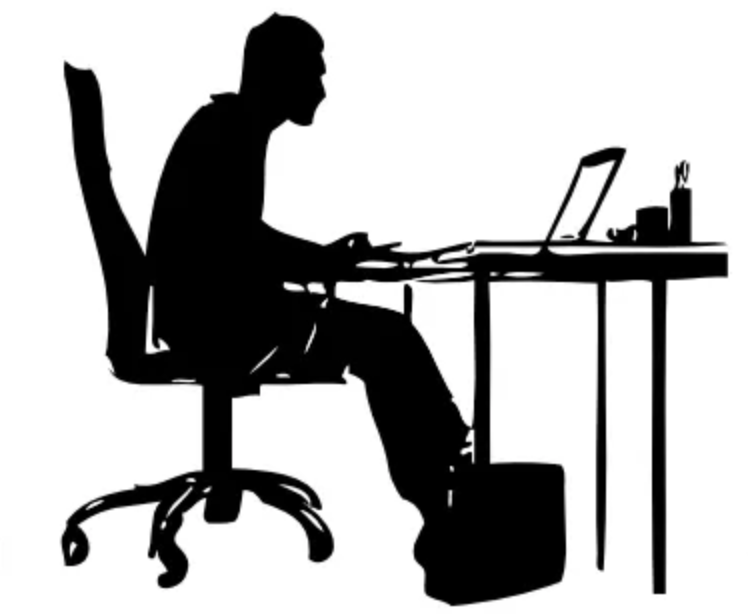
\includegraphics[width=93.45pt,height=70.5pt]{oracle_annotator.png}};
%Flowchart: Internal Storage [id:dp5388164283363912] 
\draw  [fill={rgb, 255:red, 245; green, 166; blue, 35 }  ,fill opacity=0.78 ] (728,79.73) -- (884,79.73) -- (884,168.27) -- (728,168.27) -- cycle ; \draw   (747.5,79.73) -- (747.5,168.27) ; \draw   (728,90.8) -- (884,90.8) ;
%Flowchart: Internal Storage [id:dp9110109330986611] 
\draw  [fill={rgb, 255:red, 184; green, 233; blue, 134 }  ,fill opacity=1 ] (550.67,96.31) -- (648.31,96.31) -- (648.31,185.07) -- (550.67,185.07) -- cycle ; \draw   (562.87,96.31) -- (562.87,185.07) ; \draw   (550.67,107.4) -- (648.31,107.4) ;
%Flowchart: Internal Storage [id:dp8378448524416073] 
\draw  [fill={rgb, 255:red, 74; green, 144; blue, 226 }  ,fill opacity=1 ] (518.67,81.85) -- (627.53,81.85) -- (627.53,170.61) -- (518.67,170.61) -- cycle ; \draw   (532.28,81.85) -- (532.28,170.61) ; \draw   (518.67,92.95) -- (627.53,92.95) ;
%Flowchart: Internal Storage [id:dp2773511969815008] 
\draw  [fill={rgb, 255:red, 80; green, 227; blue, 194 }  ,fill opacity=1 ] (478.67,62.93) -- (610.67,62.93) -- (610.67,153.6) -- (478.67,153.6) -- cycle ; \draw   (495.17,62.93) -- (495.17,153.6) ; \draw   (478.67,74.27) -- (610.67,74.27) ;
%Right Arrow [id:dp24273384688811261] 
\draw  [fill={rgb, 255:red, 248; green, 118; blue, 109 }  ,fill opacity=1 ] (774.67,257.11) -- (830.67,257.11) -- (830.67,250.26) -- (845.33,263.96) -- (830.67,277.66) -- (830.67,270.81) -- (774.67,270.81) -- cycle ;
%Shape: Ellipse [id:dp04390368865513983] 
\draw  [color={rgb, 255:red, 74; green, 74; blue, 74 }  ,draw opacity=1 ][fill={rgb, 255:red, 208; green, 2; blue, 27 }  ,fill opacity=0.82 ][line width=0.75]  (937.96,227.6) .. controls (937.96,220.95) and (942.58,215.55) .. (948.27,215.55) .. controls (953.97,215.55) and (958.59,220.95) .. (958.59,227.6) .. controls (958.59,234.26) and (953.97,239.65) .. (948.27,239.65) .. controls (942.58,239.65) and (937.96,234.26) .. (937.96,227.6) -- cycle ;
%Shape: Ellipse [id:dp8717410761696047] 
\draw  [color={rgb, 255:red, 74; green, 74; blue, 74 }  ,draw opacity=1 ][fill={rgb, 255:red, 208; green, 2; blue, 27 }  ,fill opacity=0.85 ][line width=0.75]  (937.96,262.05) .. controls (937.96,255.39) and (942.58,250) .. (948.27,250) .. controls (953.97,250) and (958.59,255.39) .. (958.59,262.05) .. controls (958.59,268.7) and (953.97,274.1) .. (948.27,274.1) .. controls (942.58,274.1) and (937.96,268.7) .. (937.96,262.05) -- cycle ;
%Shape: Ellipse [id:dp508980552832891] 
\draw  [color={rgb, 255:red, 74; green, 74; blue, 74 }  ,draw opacity=1 ][fill={rgb, 255:red, 208; green, 2; blue, 27 }  ,fill opacity=0.7 ][line width=0.75]  (938.51,296.77) .. controls (938.51,290.48) and (942.88,285.37) .. (948.27,285.37) .. controls (953.67,285.37) and (958.04,290.48) .. (958.04,296.77) .. controls (958.04,303.07) and (953.67,308.18) .. (948.27,308.18) .. controls (942.88,308.18) and (938.51,303.07) .. (938.51,296.77) -- cycle ;
%Straight Lines [id:da02320782495050966] 
\draw [color={rgb, 255:red, 74; green, 74; blue, 74 }  ,draw opacity=1 ][fill={rgb, 255:red, 208; green, 2; blue, 27 }  ,fill opacity=1 ][line width=0.75]    (846.79,212.32) -- (866.22,212.7) ;
\draw [shift={(868.22,212.74)}, rotate = 181.1] [color={rgb, 255:red, 74; green, 74; blue, 74 }  ,draw opacity=1 ][line width=0.75]    (10.93,-3.29) .. controls (6.95,-1.4) and (3.31,-0.3) .. (0,0) .. controls (3.31,0.3) and (6.95,1.4) .. (10.93,3.29)   ;
%Shape: Ellipse [id:dp7845135104905505] 
\draw  [color={rgb, 255:red, 74; green, 74; blue, 74 }  ,draw opacity=1 ][fill={rgb, 255:red, 208; green, 2; blue, 27 }  ,fill opacity=0.54 ][line width=0.75]  (868.22,212.74) .. controls (868.22,206.29) and (872.69,201.07) .. (878.21,201.07) .. controls (883.73,201.07) and (888.2,206.29) .. (888.2,212.74) .. controls (888.2,219.18) and (883.73,224.4) .. (878.21,224.4) .. controls (872.69,224.4) and (868.22,219.18) .. (868.22,212.74) -- cycle ;
%Shape: Ellipse [id:dp6799322828692189] 
\draw  [color={rgb, 255:red, 74; green, 74; blue, 74 }  ,draw opacity=1 ][fill={rgb, 255:red, 208; green, 2; blue, 27 }  ,fill opacity=0.66 ][line width=0.75]  (868.22,245.88) .. controls (868.22,239.23) and (872.84,233.84) .. (878.53,233.84) .. controls (884.23,233.84) and (888.85,239.23) .. (888.85,245.88) .. controls (888.85,252.54) and (884.23,257.93) .. (878.53,257.93) .. controls (872.84,257.93) and (868.22,252.54) .. (868.22,245.88) -- cycle ;
%Shape: Ellipse [id:dp9488906358304108] 
\draw  [color={rgb, 255:red, 74; green, 74; blue, 74 }  ,draw opacity=1 ][fill={rgb, 255:red, 208; green, 2; blue, 27 }  ,fill opacity=0.54 ][line width=0.75]  (868.22,277.38) .. controls (868.22,271.08) and (872.59,265.98) .. (877.98,265.98) .. controls (883.37,265.98) and (887.74,271.08) .. (887.74,277.38) .. controls (887.74,283.68) and (883.37,288.78) .. (877.98,288.78) .. controls (872.59,288.78) and (868.22,283.68) .. (868.22,277.38) -- cycle ;
%Shape: Ellipse [id:dp7098946465448284] 
\draw  [color={rgb, 255:red, 74; green, 74; blue, 74 }  ,draw opacity=1 ][fill={rgb, 255:red, 208; green, 2; blue, 27 }  ,fill opacity=0.35 ][line width=0.75]  (867.66,310.35) .. controls (867.66,303.7) and (872.28,298.3) .. (877.98,298.3) .. controls (883.68,298.3) and (888.3,303.7) .. (888.3,310.35) .. controls (888.3,317.01) and (883.68,322.4) .. (877.98,322.4) .. controls (872.28,322.4) and (867.66,317.01) .. (867.66,310.35) -- cycle ;
%Shape: Ellipse [id:dp3064810080185325] 
\draw  [color={rgb, 255:red, 74; green, 74; blue, 74 }  ,draw opacity=1 ][fill={rgb, 255:red, 208; green, 2; blue, 27 }  ,fill opacity=1 ][line width=0.75]  (988.7,262.49) .. controls (988.7,255.83) and (993.32,250.44) .. (999.02,250.44) .. controls (1004.71,250.44) and (1009.33,255.83) .. (1009.33,262.49) .. controls (1009.33,269.14) and (1004.71,274.54) .. (999.02,274.54) .. controls (993.32,274.54) and (988.7,269.14) .. (988.7,262.49) -- cycle ;
%Straight Lines [id:da2775059625363474] 
\draw [color={rgb, 255:red, 74; green, 74; blue, 74 }  ,draw opacity=1 ][fill={rgb, 255:red, 208; green, 2; blue, 27 }  ,fill opacity=1 ][line width=0.75]    (888.2,212.74) -- (936.93,223.53) ;
\draw [shift={(938.89,223.96)}, rotate = 192.48] [color={rgb, 255:red, 74; green, 74; blue, 74 }  ,draw opacity=1 ][line width=0.75]    (10.93,-3.29) .. controls (6.95,-1.4) and (3.31,-0.3) .. (0,0) .. controls (3.31,0.3) and (6.95,1.4) .. (10.93,3.29)   ;
%Straight Lines [id:da37055269984493155] 
\draw [color={rgb, 255:red, 74; green, 74; blue, 74 }  ,draw opacity=1 ][fill={rgb, 255:red, 208; green, 2; blue, 27 }  ,fill opacity=1 ][line width=0.75]    (846.79,245.47) -- (866.22,245.85) ;
\draw [shift={(868.22,245.88)}, rotate = 181.1] [color={rgb, 255:red, 74; green, 74; blue, 74 }  ,draw opacity=1 ][line width=0.75]    (10.93,-3.29) .. controls (6.95,-1.4) and (3.31,-0.3) .. (0,0) .. controls (3.31,0.3) and (6.95,1.4) .. (10.93,3.29)   ;
%Straight Lines [id:da47178511371168885] 
\draw [color={rgb, 255:red, 74; green, 74; blue, 74 }  ,draw opacity=1 ][fill={rgb, 255:red, 208; green, 2; blue, 27 }  ,fill opacity=1 ][line width=0.75]    (846.79,276.97) -- (866.22,277.34) ;
\draw [shift={(868.22,277.38)}, rotate = 181.1] [color={rgb, 255:red, 74; green, 74; blue, 74 }  ,draw opacity=1 ][line width=0.75]    (10.93,-3.29) .. controls (6.95,-1.4) and (3.31,-0.3) .. (0,0) .. controls (3.31,0.3) and (6.95,1.4) .. (10.93,3.29)   ;
%Straight Lines [id:da6004920898188288] 
\draw [color={rgb, 255:red, 74; green, 74; blue, 74 }  ,draw opacity=1 ][fill={rgb, 255:red, 208; green, 2; blue, 27 }  ,fill opacity=1 ][line width=0.75]    (888.2,212.74) -- (937.39,256.25) ;
\draw [shift={(938.89,257.57)}, rotate = 221.5] [color={rgb, 255:red, 74; green, 74; blue, 74 }  ,draw opacity=1 ][line width=0.75]    (10.93,-3.29) .. controls (6.95,-1.4) and (3.31,-0.3) .. (0,0) .. controls (3.31,0.3) and (6.95,1.4) .. (10.93,3.29)   ;
%Straight Lines [id:da5211766232179535] 
\draw [color={rgb, 255:red, 74; green, 74; blue, 74 }  ,draw opacity=1 ][fill={rgb, 255:red, 208; green, 2; blue, 27 }  ,fill opacity=1 ][line width=0.75]    (888.2,212.74) -- (938.89,289.52) ;
\draw [shift={(939.99,291.19)}, rotate = 236.57] [color={rgb, 255:red, 74; green, 74; blue, 74 }  ,draw opacity=1 ][line width=0.75]    (10.93,-3.29) .. controls (6.95,-1.4) and (3.31,-0.3) .. (0,0) .. controls (3.31,0.3) and (6.95,1.4) .. (10.93,3.29)   ;
%Straight Lines [id:da7487942741190119] 
\draw [color={rgb, 255:red, 74; green, 74; blue, 74 }  ,draw opacity=1 ][fill={rgb, 255:red, 208; green, 2; blue, 27 }  ,fill opacity=1 ][line width=0.75]    (888.85,245.88) -- (936.08,228.3) ;
\draw [shift={(937.96,227.6)}, rotate = 159.58] [color={rgb, 255:red, 74; green, 74; blue, 74 }  ,draw opacity=1 ][line width=0.75]    (10.93,-3.29) .. controls (6.95,-1.4) and (3.31,-0.3) .. (0,0) .. controls (3.31,0.3) and (6.95,1.4) .. (10.93,3.29)   ;
%Straight Lines [id:da8181641007104268] 
\draw [color={rgb, 255:red, 74; green, 74; blue, 74 }  ,draw opacity=1 ][fill={rgb, 255:red, 208; green, 2; blue, 27 }  ,fill opacity=1 ][line width=0.75]    (888.85,245.88) -- (936.06,261.42) ;
\draw [shift={(937.96,262.05)}, rotate = 198.22] [color={rgb, 255:red, 74; green, 74; blue, 74 }  ,draw opacity=1 ][line width=0.75]    (10.93,-3.29) .. controls (6.95,-1.4) and (3.31,-0.3) .. (0,0) .. controls (3.31,0.3) and (6.95,1.4) .. (10.93,3.29)   ;
%Straight Lines [id:da36425475389367556] 
\draw [color={rgb, 255:red, 74; green, 74; blue, 74 }  ,draw opacity=1 ][fill={rgb, 255:red, 208; green, 2; blue, 27 }  ,fill opacity=1 ][line width=0.75]    (888.85,245.88) -- (937.11,295.34) ;
\draw [shift={(938.51,296.77)}, rotate = 225.7] [color={rgb, 255:red, 74; green, 74; blue, 74 }  ,draw opacity=1 ][line width=0.75]    (10.93,-3.29) .. controls (6.95,-1.4) and (3.31,-0.3) .. (0,0) .. controls (3.31,0.3) and (6.95,1.4) .. (10.93,3.29)   ;
%Straight Lines [id:da737661820158507] 
\draw [color={rgb, 255:red, 74; green, 74; blue, 74 }  ,draw opacity=1 ][fill={rgb, 255:red, 208; green, 2; blue, 27 }  ,fill opacity=1 ][line width=0.75]    (887.74,277.38) -- (937.07,300.05) ;
\draw [shift={(938.89,300.89)}, rotate = 204.68] [color={rgb, 255:red, 74; green, 74; blue, 74 }  ,draw opacity=1 ][line width=0.75]    (10.93,-3.29) .. controls (6.95,-1.4) and (3.31,-0.3) .. (0,0) .. controls (3.31,0.3) and (6.95,1.4) .. (10.93,3.29)   ;
%Straight Lines [id:da12920698569256395] 
\draw [color={rgb, 255:red, 74; green, 74; blue, 74 }  ,draw opacity=1 ][fill={rgb, 255:red, 208; green, 2; blue, 27 }  ,fill opacity=1 ][line width=0.75]    (888.3,310.35) -- (938.56,304.36) ;
\draw [shift={(940.55,304.12)}, rotate = 173.2] [color={rgb, 255:red, 74; green, 74; blue, 74 }  ,draw opacity=1 ][line width=0.75]    (10.93,-3.29) .. controls (6.95,-1.4) and (3.31,-0.3) .. (0,0) .. controls (3.31,0.3) and (6.95,1.4) .. (10.93,3.29)   ;
%Straight Lines [id:da18467172352070604] 
\draw [color={rgb, 255:red, 74; green, 74; blue, 74 }  ,draw opacity=1 ][fill={rgb, 255:red, 208; green, 2; blue, 27 }  ,fill opacity=1 ][line width=0.75]    (887.74,277.38) -- (936.94,265.79) ;
\draw [shift={(938.89,265.33)}, rotate = 166.74] [color={rgb, 255:red, 74; green, 74; blue, 74 }  ,draw opacity=1 ][line width=0.75]    (10.93,-3.29) .. controls (6.95,-1.4) and (3.31,-0.3) .. (0,0) .. controls (3.31,0.3) and (6.95,1.4) .. (10.93,3.29)   ;
%Straight Lines [id:da9466499071617294] 
\draw [color={rgb, 255:red, 74; green, 74; blue, 74 }  ,draw opacity=1 ][fill={rgb, 255:red, 208; green, 2; blue, 27 }  ,fill opacity=1 ][line width=0.75]    (888.3,310.35) -- (938.43,270.46) ;
\draw [shift={(939.99,269.21)}, rotate = 141.49] [color={rgb, 255:red, 74; green, 74; blue, 74 }  ,draw opacity=1 ][line width=0.75]    (10.93,-3.29) .. controls (6.95,-1.4) and (3.31,-0.3) .. (0,0) .. controls (3.31,0.3) and (6.95,1.4) .. (10.93,3.29)   ;
%Straight Lines [id:da4506241894804748] 
\draw [color={rgb, 255:red, 74; green, 74; blue, 74 }  ,draw opacity=1 ][fill={rgb, 255:red, 208; green, 2; blue, 27 }  ,fill opacity=1 ][line width=0.75]    (888.3,310.35) -- (938.86,236.6) ;
\draw [shift={(939.99,234.95)}, rotate = 124.43] [color={rgb, 255:red, 74; green, 74; blue, 74 }  ,draw opacity=1 ][line width=0.75]    (10.93,-3.29) .. controls (6.95,-1.4) and (3.31,-0.3) .. (0,0) .. controls (3.31,0.3) and (6.95,1.4) .. (10.93,3.29)   ;
%Straight Lines [id:da2221864135550169] 
\draw [color={rgb, 255:red, 74; green, 74; blue, 74 }  ,draw opacity=1 ][fill={rgb, 255:red, 208; green, 2; blue, 27 }  ,fill opacity=1 ][line width=0.75]    (888.02,277.11) -- (937.31,232.17) ;
\draw [shift={(938.79,230.82)}, rotate = 137.65] [color={rgb, 255:red, 74; green, 74; blue, 74 }  ,draw opacity=1 ][line width=0.75]    (10.93,-3.29) .. controls (6.95,-1.4) and (3.31,-0.3) .. (0,0) .. controls (3.31,0.3) and (6.95,1.4) .. (10.93,3.29)   ;
%Straight Lines [id:da003134524188506349] 
\draw [color={rgb, 255:red, 74; green, 74; blue, 74 }  ,draw opacity=1 ][fill={rgb, 255:red, 208; green, 2; blue, 27 }  ,fill opacity=1 ][line width=0.75]    (958.59,227.6) -- (992.06,251.62) ;
\draw [shift={(993.68,252.79)}, rotate = 215.67] [color={rgb, 255:red, 74; green, 74; blue, 74 }  ,draw opacity=1 ][line width=0.75]    (10.93,-3.29) .. controls (6.95,-1.4) and (3.31,-0.3) .. (0,0) .. controls (3.31,0.3) and (6.95,1.4) .. (10.93,3.29)   ;
%Straight Lines [id:da4998698569165574] 
\draw [color={rgb, 255:red, 74; green, 74; blue, 74 }  ,draw opacity=1 ][fill={rgb, 255:red, 208; green, 2; blue, 27 }  ,fill opacity=1 ][line width=0.75]    (958.59,262.05) -- (986.7,262.46) ;
\draw [shift={(988.7,262.49)}, rotate = 180.84] [color={rgb, 255:red, 74; green, 74; blue, 74 }  ,draw opacity=1 ][line width=0.75]    (10.93,-3.29) .. controls (6.95,-1.4) and (3.31,-0.3) .. (0,0) .. controls (3.31,0.3) and (6.95,1.4) .. (10.93,3.29)   ;
%Straight Lines [id:da2775073313106582] 
\draw [color={rgb, 255:red, 74; green, 74; blue, 74 }  ,draw opacity=1 ][fill={rgb, 255:red, 208; green, 2; blue, 27 }  ,fill opacity=1 ][line width=0.75]    (958.04,296.77) -- (990.97,272.09) ;
\draw [shift={(992.57,270.89)}, rotate = 143.15] [color={rgb, 255:red, 74; green, 74; blue, 74 }  ,draw opacity=1 ][line width=0.75]    (10.93,-3.29) .. controls (6.95,-1.4) and (3.31,-0.3) .. (0,0) .. controls (3.31,0.3) and (6.95,1.4) .. (10.93,3.29)   ;
%Straight Lines [id:da6380577812271726] 
\draw [color={rgb, 255:red, 74; green, 74; blue, 74 }  ,draw opacity=1 ][fill={rgb, 255:red, 208; green, 2; blue, 27 }  ,fill opacity=1 ][line width=0.75]    (846.23,309.94) -- (865.66,310.31) ;
\draw [shift={(867.66,310.35)}, rotate = 181.1] [color={rgb, 255:red, 74; green, 74; blue, 74 }  ,draw opacity=1 ][line width=0.75]    (10.93,-3.29) .. controls (6.95,-1.4) and (3.31,-0.3) .. (0,0) .. controls (3.31,0.3) and (6.95,1.4) .. (10.93,3.29)   ;

%Shape: Ellipse [id:dp0949991368526919] 
\draw  [color={rgb, 255:red, 74; green, 74; blue, 74 }  ,draw opacity=1 ][fill={rgb, 255:red, 245; green, 166; blue, 35 }  ,fill opacity=1 ][line width=0.75]  (696.62,227.6) .. controls (696.62,220.95) and (701.24,215.55) .. (706.94,215.55) .. controls (712.64,215.55) and (717.26,220.95) .. (717.26,227.6) .. controls (717.26,234.26) and (712.64,239.65) .. (706.94,239.65) .. controls (701.24,239.65) and (696.62,234.26) .. (696.62,227.6) -- cycle ;
%Shape: Ellipse [id:dp17917851929491002] 
\draw  [color={rgb, 255:red, 74; green, 74; blue, 74 }  ,draw opacity=1 ][fill={rgb, 255:red, 245; green, 166; blue, 35 }  ,fill opacity=1 ][line width=0.75]  (696.62,262.05) .. controls (696.62,255.39) and (701.24,250) .. (706.94,250) .. controls (712.64,250) and (717.26,255.39) .. (717.26,262.05) .. controls (717.26,268.7) and (712.64,274.1) .. (706.94,274.1) .. controls (701.24,274.1) and (696.62,268.7) .. (696.62,262.05) -- cycle ;
%Shape: Ellipse [id:dp6468398049913187] 
\draw  [color={rgb, 255:red, 74; green, 74; blue, 74 }  ,draw opacity=1 ][fill={rgb, 255:red, 245; green, 166; blue, 35 }  ,fill opacity=1 ][line width=0.75]  (697.18,296.77) .. controls (697.18,290.48) and (701.55,285.37) .. (706.94,285.37) .. controls (712.33,285.37) and (716.7,290.48) .. (716.7,296.77) .. controls (716.7,303.07) and (712.33,308.18) .. (706.94,308.18) .. controls (701.55,308.18) and (697.18,303.07) .. (697.18,296.77) -- cycle ;
%Straight Lines [id:da33649013863325306] 
\draw [color={rgb, 255:red, 74; green, 74; blue, 74 }  ,draw opacity=1 ][fill={rgb, 255:red, 245; green, 166; blue, 35 }  ,fill opacity=1 ][line width=0.75]    (605.45,212.32) -- (624.88,212.7) ;
\draw [shift={(626.88,212.74)}, rotate = 181.1] [color={rgb, 255:red, 74; green, 74; blue, 74 }  ,draw opacity=1 ][line width=0.75]    (10.93,-3.29) .. controls (6.95,-1.4) and (3.31,-0.3) .. (0,0) .. controls (3.31,0.3) and (6.95,1.4) .. (10.93,3.29)   ;
%Shape: Ellipse [id:dp024275059589674575] 
\draw  [color={rgb, 255:red, 74; green, 74; blue, 74 }  ,draw opacity=1 ][fill={rgb, 255:red, 245; green, 166; blue, 35 }  ,fill opacity=1 ][line width=0.75]  (626.88,212.74) .. controls (626.88,206.29) and (631.36,201.07) .. (636.87,201.07) .. controls (642.39,201.07) and (646.87,206.29) .. (646.87,212.74) .. controls (646.87,219.18) and (642.39,224.4) .. (636.87,224.4) .. controls (631.36,224.4) and (626.88,219.18) .. (626.88,212.74) -- cycle ;
%Shape: Ellipse [id:dp922936288798959] 
\draw  [color={rgb, 255:red, 74; green, 74; blue, 74 }  ,draw opacity=1 ][fill={rgb, 255:red, 245; green, 166; blue, 35 }  ,fill opacity=1 ][line width=0.75]  (626.88,245.88) .. controls (626.88,239.23) and (631.5,233.84) .. (637.2,233.84) .. controls (642.9,233.84) and (647.52,239.23) .. (647.52,245.88) .. controls (647.52,252.54) and (642.9,257.93) .. (637.2,257.93) .. controls (631.5,257.93) and (626.88,252.54) .. (626.88,245.88) -- cycle ;
%Shape: Ellipse [id:dp11094438567990372] 
\draw  [color={rgb, 255:red, 74; green, 74; blue, 74 }  ,draw opacity=1 ][fill={rgb, 255:red, 245; green, 166; blue, 35 }  ,fill opacity=1 ][line width=0.75]  (626.88,277.38) .. controls (626.88,271.08) and (631.26,265.98) .. (636.65,265.98) .. controls (642.04,265.98) and (646.41,271.08) .. (646.41,277.38) .. controls (646.41,283.68) and (642.04,288.78) .. (636.65,288.78) .. controls (631.26,288.78) and (626.88,283.68) .. (626.88,277.38) -- cycle ;
%Shape: Ellipse [id:dp7655203583891028] 
\draw  [color={rgb, 255:red, 74; green, 74; blue, 74 }  ,draw opacity=1 ][fill={rgb, 255:red, 245; green, 166; blue, 35 }  ,fill opacity=1 ][line width=0.75]  (626.33,310.35) .. controls (626.33,303.7) and (630.95,298.3) .. (636.65,298.3) .. controls (642.34,298.3) and (646.96,303.7) .. (646.96,310.35) .. controls (646.96,317.01) and (642.34,322.4) .. (636.65,322.4) .. controls (630.95,322.4) and (626.33,317.01) .. (626.33,310.35) -- cycle ;
%Shape: Ellipse [id:dp4803791816333616] 
\draw  [color={rgb, 255:red, 74; green, 74; blue, 74 }  ,draw opacity=1 ][fill={rgb, 255:red, 245; green, 166; blue, 35 }  ,fill opacity=1 ][line width=0.75]  (747.37,262.49) .. controls (747.37,255.83) and (751.99,250.44) .. (757.68,250.44) .. controls (763.38,250.44) and (768,255.83) .. (768,262.49) .. controls (768,269.14) and (763.38,274.54) .. (757.68,274.54) .. controls (751.99,274.54) and (747.37,269.14) .. (747.37,262.49) -- cycle ;
%Straight Lines [id:da831345251674658] 
\draw [color={rgb, 255:red, 74; green, 74; blue, 74 }  ,draw opacity=1 ][fill={rgb, 255:red, 245; green, 166; blue, 35 }  ,fill opacity=1 ][line width=0.75]    (646.87,212.74) -- (695.6,223.53) ;
\draw [shift={(697.55,223.96)}, rotate = 192.48] [color={rgb, 255:red, 74; green, 74; blue, 74 }  ,draw opacity=1 ][line width=0.75]    (10.93,-3.29) .. controls (6.95,-1.4) and (3.31,-0.3) .. (0,0) .. controls (3.31,0.3) and (6.95,1.4) .. (10.93,3.29)   ;
%Straight Lines [id:da42235669596798564] 
\draw [color={rgb, 255:red, 74; green, 74; blue, 74 }  ,draw opacity=1 ][fill={rgb, 255:red, 245; green, 166; blue, 35 }  ,fill opacity=1 ][line width=0.75]    (605.45,245.47) -- (624.88,245.85) ;
\draw [shift={(626.88,245.88)}, rotate = 181.1] [color={rgb, 255:red, 74; green, 74; blue, 74 }  ,draw opacity=1 ][line width=0.75]    (10.93,-3.29) .. controls (6.95,-1.4) and (3.31,-0.3) .. (0,0) .. controls (3.31,0.3) and (6.95,1.4) .. (10.93,3.29)   ;
%Straight Lines [id:da25179477875208667] 
\draw [color={rgb, 255:red, 74; green, 74; blue, 74 }  ,draw opacity=1 ][fill={rgb, 255:red, 245; green, 166; blue, 35 }  ,fill opacity=1 ][line width=0.75]    (605.45,276.97) -- (624.88,277.34) ;
\draw [shift={(626.88,277.38)}, rotate = 181.1] [color={rgb, 255:red, 74; green, 74; blue, 74 }  ,draw opacity=1 ][line width=0.75]    (10.93,-3.29) .. controls (6.95,-1.4) and (3.31,-0.3) .. (0,0) .. controls (3.31,0.3) and (6.95,1.4) .. (10.93,3.29)   ;
%Straight Lines [id:da22700462503924546] 
\draw [color={rgb, 255:red, 74; green, 74; blue, 74 }  ,draw opacity=1 ][fill={rgb, 255:red, 245; green, 166; blue, 35 }  ,fill opacity=1 ][line width=0.75]    (646.87,212.74) -- (696.05,256.25) ;
\draw [shift={(697.55,257.57)}, rotate = 221.5] [color={rgb, 255:red, 74; green, 74; blue, 74 }  ,draw opacity=1 ][line width=0.75]    (10.93,-3.29) .. controls (6.95,-1.4) and (3.31,-0.3) .. (0,0) .. controls (3.31,0.3) and (6.95,1.4) .. (10.93,3.29)   ;
%Straight Lines [id:da8929430986730775] 
\draw [color={rgb, 255:red, 74; green, 74; blue, 74 }  ,draw opacity=1 ][fill={rgb, 255:red, 245; green, 166; blue, 35 }  ,fill opacity=1 ][line width=0.75]    (646.87,212.74) -- (697.56,289.52) ;
\draw [shift={(698.66,291.19)}, rotate = 236.57] [color={rgb, 255:red, 74; green, 74; blue, 74 }  ,draw opacity=1 ][line width=0.75]    (10.93,-3.29) .. controls (6.95,-1.4) and (3.31,-0.3) .. (0,0) .. controls (3.31,0.3) and (6.95,1.4) .. (10.93,3.29)   ;
%Straight Lines [id:da9581300224008351] 
\draw [color={rgb, 255:red, 74; green, 74; blue, 74 }  ,draw opacity=1 ][fill={rgb, 255:red, 245; green, 166; blue, 35 }  ,fill opacity=1 ][line width=0.75]    (647.52,245.88) -- (694.75,228.3) ;
\draw [shift={(696.62,227.6)}, rotate = 159.58] [color={rgb, 255:red, 74; green, 74; blue, 74 }  ,draw opacity=1 ][line width=0.75]    (10.93,-3.29) .. controls (6.95,-1.4) and (3.31,-0.3) .. (0,0) .. controls (3.31,0.3) and (6.95,1.4) .. (10.93,3.29)   ;
%Straight Lines [id:da2870674546040919] 
\draw [color={rgb, 255:red, 74; green, 74; blue, 74 }  ,draw opacity=1 ][fill={rgb, 255:red, 245; green, 166; blue, 35 }  ,fill opacity=1 ][line width=0.75]    (647.52,245.88) -- (694.72,261.42) ;
\draw [shift={(696.62,262.05)}, rotate = 198.22] [color={rgb, 255:red, 74; green, 74; blue, 74 }  ,draw opacity=1 ][line width=0.75]    (10.93,-3.29) .. controls (6.95,-1.4) and (3.31,-0.3) .. (0,0) .. controls (3.31,0.3) and (6.95,1.4) .. (10.93,3.29)   ;
%Straight Lines [id:da3654757597156302] 
\draw [color={rgb, 255:red, 74; green, 74; blue, 74 }  ,draw opacity=1 ][fill={rgb, 255:red, 245; green, 166; blue, 35 }  ,fill opacity=1 ][line width=0.75]    (647.52,245.88) -- (695.78,295.34) ;
\draw [shift={(697.18,296.77)}, rotate = 225.7] [color={rgb, 255:red, 74; green, 74; blue, 74 }  ,draw opacity=1 ][line width=0.75]    (10.93,-3.29) .. controls (6.95,-1.4) and (3.31,-0.3) .. (0,0) .. controls (3.31,0.3) and (6.95,1.4) .. (10.93,3.29)   ;
%Straight Lines [id:da0913587825231239] 
\draw [color={rgb, 255:red, 74; green, 74; blue, 74 }  ,draw opacity=1 ][fill={rgb, 255:red, 245; green, 166; blue, 35 }  ,fill opacity=1 ][line width=0.75]    (646.41,277.38) -- (695.74,300.05) ;
\draw [shift={(697.55,300.89)}, rotate = 204.68] [color={rgb, 255:red, 74; green, 74; blue, 74 }  ,draw opacity=1 ][line width=0.75]    (10.93,-3.29) .. controls (6.95,-1.4) and (3.31,-0.3) .. (0,0) .. controls (3.31,0.3) and (6.95,1.4) .. (10.93,3.29)   ;
%Straight Lines [id:da314169300024961] 
\draw [color={rgb, 255:red, 74; green, 74; blue, 74 }  ,draw opacity=1 ][fill={rgb, 255:red, 245; green, 166; blue, 35 }  ,fill opacity=1 ][line width=0.75]    (646.96,310.35) -- (697.23,304.36) ;
\draw [shift={(699.21,304.12)}, rotate = 173.2] [color={rgb, 255:red, 74; green, 74; blue, 74 }  ,draw opacity=1 ][line width=0.75]    (10.93,-3.29) .. controls (6.95,-1.4) and (3.31,-0.3) .. (0,0) .. controls (3.31,0.3) and (6.95,1.4) .. (10.93,3.29)   ;
%Straight Lines [id:da12360398129849459] 
\draw [color={rgb, 255:red, 74; green, 74; blue, 74 }  ,draw opacity=1 ][fill={rgb, 255:red, 245; green, 166; blue, 35 }  ,fill opacity=1 ][line width=0.75]    (646.41,277.38) -- (695.61,265.79) ;
\draw [shift={(697.55,265.33)}, rotate = 166.74] [color={rgb, 255:red, 74; green, 74; blue, 74 }  ,draw opacity=1 ][line width=0.75]    (10.93,-3.29) .. controls (6.95,-1.4) and (3.31,-0.3) .. (0,0) .. controls (3.31,0.3) and (6.95,1.4) .. (10.93,3.29)   ;
%Straight Lines [id:da9605922373604874] 
\draw [color={rgb, 255:red, 74; green, 74; blue, 74 }  ,draw opacity=1 ][fill={rgb, 255:red, 245; green, 166; blue, 35 }  ,fill opacity=1 ][line width=0.75]    (646.96,310.35) -- (697.09,270.46) ;
\draw [shift={(698.66,269.21)}, rotate = 141.49] [color={rgb, 255:red, 74; green, 74; blue, 74 }  ,draw opacity=1 ][line width=0.75]    (10.93,-3.29) .. controls (6.95,-1.4) and (3.31,-0.3) .. (0,0) .. controls (3.31,0.3) and (6.95,1.4) .. (10.93,3.29)   ;
%Straight Lines [id:da1432593832160851] 
\draw [color={rgb, 255:red, 74; green, 74; blue, 74 }  ,draw opacity=1 ][fill={rgb, 255:red, 245; green, 166; blue, 35 }  ,fill opacity=1 ][line width=0.75]    (646.96,310.35) -- (697.53,236.6) ;
\draw [shift={(698.66,234.95)}, rotate = 124.43] [color={rgb, 255:red, 74; green, 74; blue, 74 }  ,draw opacity=1 ][line width=0.75]    (10.93,-3.29) .. controls (6.95,-1.4) and (3.31,-0.3) .. (0,0) .. controls (3.31,0.3) and (6.95,1.4) .. (10.93,3.29)   ;
%Straight Lines [id:da3037075535291185] 
\draw [color={rgb, 255:red, 74; green, 74; blue, 74 }  ,draw opacity=1 ][fill={rgb, 255:red, 245; green, 166; blue, 35 }  ,fill opacity=1 ][line width=0.75]    (646.78,277.35) -- (696.07,232.42) ;
\draw [shift={(697.55,231.07)}, rotate = 137.65] [color={rgb, 255:red, 74; green, 74; blue, 74 }  ,draw opacity=1 ][line width=0.75]    (10.93,-3.29) .. controls (6.95,-1.4) and (3.31,-0.3) .. (0,0) .. controls (3.31,0.3) and (6.95,1.4) .. (10.93,3.29)   ;
%Straight Lines [id:da7803989270968215] 
\draw [color={rgb, 255:red, 74; green, 74; blue, 74 }  ,draw opacity=1 ][fill={rgb, 255:red, 245; green, 166; blue, 35 }  ,fill opacity=1 ][line width=0.75]    (717.26,227.6) -- (750.72,251.62) ;
\draw [shift={(752.35,252.79)}, rotate = 215.67] [color={rgb, 255:red, 74; green, 74; blue, 74 }  ,draw opacity=1 ][line width=0.75]    (10.93,-3.29) .. controls (6.95,-1.4) and (3.31,-0.3) .. (0,0) .. controls (3.31,0.3) and (6.95,1.4) .. (10.93,3.29)   ;
%Straight Lines [id:da41130243392517696] 
\draw [color={rgb, 255:red, 74; green, 74; blue, 74 }  ,draw opacity=1 ][fill={rgb, 255:red, 245; green, 166; blue, 35 }  ,fill opacity=1 ][line width=0.75]    (717.26,262.05) -- (745.37,262.46) ;
\draw [shift={(747.37,262.49)}, rotate = 180.84] [color={rgb, 255:red, 74; green, 74; blue, 74 }  ,draw opacity=1 ][line width=0.75]    (10.93,-3.29) .. controls (6.95,-1.4) and (3.31,-0.3) .. (0,0) .. controls (3.31,0.3) and (6.95,1.4) .. (10.93,3.29)   ;
%Straight Lines [id:da45227299504650254] 
\draw [color={rgb, 255:red, 74; green, 74; blue, 74 }  ,draw opacity=1 ][fill={rgb, 255:red, 245; green, 166; blue, 35 }  ,fill opacity=1 ][line width=0.75]    (716.7,296.77) -- (749.64,272.09) ;
\draw [shift={(751.24,270.89)}, rotate = 143.15] [color={rgb, 255:red, 74; green, 74; blue, 74 }  ,draw opacity=1 ][line width=0.75]    (10.93,-3.29) .. controls (6.95,-1.4) and (3.31,-0.3) .. (0,0) .. controls (3.31,0.3) and (6.95,1.4) .. (10.93,3.29)   ;
%Straight Lines [id:da28353551872522686] 
\draw [color={rgb, 255:red, 74; green, 74; blue, 74 }  ,draw opacity=1 ][fill={rgb, 255:red, 245; green, 166; blue, 35 }  ,fill opacity=1 ][line width=0.75]    (604.9,309.94) -- (624.33,310.31) ;
\draw [shift={(626.33,310.35)}, rotate = 181.1] [color={rgb, 255:red, 74; green, 74; blue, 74 }  ,draw opacity=1 ][line width=0.75]    (10.93,-3.29) .. controls (6.95,-1.4) and (3.31,-0.3) .. (0,0) .. controls (3.31,0.3) and (6.95,1.4) .. (10.93,3.29)   ;

%Bend Arrow [id:dp7761411179753315] 
\draw  [fill={rgb, 255:red, 248; green, 118; blue, 109 }  ,fill opacity=0.87 ] (647.98,126.66) -- (666.19,126.49) .. controls (681.28,126.35) and (693.62,138.47) .. (693.76,153.55) -- (694.08,187.81) -- (699.14,187.77) -- (686.66,206.66) -- (673.84,188) -- (678.9,187.95) -- (678.58,153.69) .. controls (678.52,146.99) and (673.04,141.6) .. (666.33,141.67) -- (648.12,141.83) -- cycle ;
%Straight Lines [id:da5718585891491981] 
\draw    (807.45,170.32) -- (807.99,255.07) ;
\draw [shift={(808,257.07)}, rotate = 269.64] [color={rgb, 255:red, 0; green, 0; blue, 0 }  ][line width=0.75]    (10.93,-3.29) .. controls (6.95,-1.4) and (3.31,-0.3) .. (0,0) .. controls (3.31,0.3) and (6.95,1.4) .. (10.93,3.29)   ;
%Right Arrow [id:dp26022490978484436] 
\draw  [fill={rgb, 255:red, 248; green, 118; blue, 109 }  ,fill opacity=1 ] (414.68,739.18) -- (325.51,739.71) -- (325.55,746.56) -- (302.11,733) -- (325.38,719.16) -- (325.43,726.01) -- (414.6,725.48) -- cycle ;
%Right Arrow [id:dp3707461154684315] 
\draw  [fill={rgb, 255:red, 248; green, 118; blue, 109 }  ,fill opacity=1 ] (236.5,684.8) -- (236.83,620.33) -- (229.98,620.3) -- (243.76,603.48) -- (257.38,620.44) -- (250.53,620.4) -- (250.2,684.87) -- cycle ;
%Shape: Ellipse [id:dp22799781372843708] 
\draw  [color={rgb, 255:red, 74; green, 74; blue, 74 }  ,draw opacity=1 ][fill={rgb, 255:red, 208; green, 2; blue, 27 }  ,fill opacity=0.82 ][line width=0.75]  (220.86,767.44) .. controls (220.92,773.36) and (216.92,778.21) .. (211.94,778.26) .. controls (206.96,778.31) and (202.87,773.54) .. (202.81,767.61) .. controls (202.76,761.68) and (206.75,756.84) .. (211.73,756.79) .. controls (216.71,756.74) and (220.8,761.51) .. (220.86,767.44) -- cycle ;
%Shape: Ellipse [id:dp0938069404277384] 
\draw  [color={rgb, 255:red, 74; green, 74; blue, 74 }  ,draw opacity=1 ][fill={rgb, 255:red, 208; green, 2; blue, 27 }  ,fill opacity=0.85 ][line width=0.75]  (220.56,736.75) .. controls (220.62,742.68) and (216.62,747.53) .. (211.64,747.58) .. controls (206.66,747.63) and (202.57,742.86) .. (202.51,736.93) .. controls (202.46,731) and (206.45,726.16) .. (211.43,726.11) .. controls (216.41,726.06) and (220.5,730.83) .. (220.56,736.75) -- cycle ;
%Shape: Ellipse [id:dp6140474972481622] 
\draw  [color={rgb, 255:red, 74; green, 74; blue, 74 }  ,draw opacity=1 ][fill={rgb, 255:red, 208; green, 2; blue, 27 }  ,fill opacity=0.7 ][line width=0.75]  (219.77,705.82) .. controls (219.83,711.43) and (216.05,716.02) .. (211.33,716.06) .. controls (206.62,716.11) and (202.75,711.6) .. (202.7,705.99) .. controls (202.64,700.38) and (206.42,695.8) .. (211.13,695.75) .. controls (215.85,695.7) and (219.72,700.21) .. (219.77,705.82) -- cycle ;
%Straight Lines [id:da06742996929615419] 
\draw [color={rgb, 255:red, 74; green, 74; blue, 74 }  ,draw opacity=1 ][fill={rgb, 255:red, 208; green, 2; blue, 27 }  ,fill opacity=1 ][line width=0.75]    (300.73,780.27) -- (283.98,780.1) ;
\draw [shift={(281.98,780.08)}, rotate = 0.57] [color={rgb, 255:red, 74; green, 74; blue, 74 }  ,draw opacity=1 ][line width=0.75]    (10.93,-3.29) .. controls (6.95,-1.4) and (3.31,-0.3) .. (0,0) .. controls (3.31,0.3) and (6.95,1.4) .. (10.93,3.29)   ;
%Shape: Ellipse [id:dp5300833041600048] 
\draw  [color={rgb, 255:red, 74; green, 74; blue, 74 }  ,draw opacity=1 ][fill={rgb, 255:red, 208; green, 2; blue, 27 }  ,fill opacity=0.54 ][line width=0.75]  (281.98,780.08) .. controls (282.03,785.82) and (278.17,790.52) .. (273.34,790.56) .. controls (268.52,790.61) and (264.56,786) .. (264.5,780.25) .. controls (264.45,774.51) and (268.31,769.82) .. (273.14,769.78) .. controls (277.96,769.73) and (281.92,774.34) .. (281.98,780.08) -- cycle ;
%Shape: Ellipse [id:dp20620413228082501] 
\draw  [color={rgb, 255:red, 74; green, 74; blue, 74 }  ,draw opacity=1 ][fill={rgb, 255:red, 208; green, 2; blue, 27 }  ,fill opacity=0.66 ][line width=0.75]  (281.69,750.56) .. controls (281.75,756.48) and (277.76,761.33) .. (272.77,761.38) .. controls (267.79,761.43) and (263.7,756.66) .. (263.64,750.73) .. controls (263.59,744.8) and (267.58,739.96) .. (272.56,739.91) .. controls (277.55,739.86) and (281.63,744.63) .. (281.69,750.56) -- cycle ;
%Shape: Ellipse [id:dp6250214667442204] 
\draw  [color={rgb, 255:red, 74; green, 74; blue, 74 }  ,draw opacity=1 ][fill={rgb, 255:red, 208; green, 2; blue, 27 }  ,fill opacity=0.54 ][line width=0.75]  (281.42,722.5) .. controls (281.47,728.11) and (277.69,732.69) .. (272.98,732.74) .. controls (268.26,732.79) and (264.39,728.28) .. (264.34,722.67) .. controls (264.28,717.06) and (268.06,712.47) .. (272.78,712.42) .. controls (277.49,712.38) and (281.36,716.89) .. (281.42,722.5) -- cycle ;
%Shape: Ellipse [id:dp6719991232981453] 
\draw  [color={rgb, 255:red, 74; green, 74; blue, 74 }  ,draw opacity=1 ][fill={rgb, 255:red, 208; green, 2; blue, 27 }  ,fill opacity=0.35 ][line width=0.75]  (281.61,693.12) .. controls (281.67,699.05) and (277.68,703.9) .. (272.69,703.95) .. controls (267.71,704) and (263.63,699.23) .. (263.57,693.3) .. controls (263.51,687.37) and (267.5,682.53) .. (272.49,682.48) .. controls (277.47,682.43) and (281.55,687.2) .. (281.61,693.12) -- cycle ;
%Shape: Ellipse [id:dp7508533952034346] 
\draw  [color={rgb, 255:red, 74; green, 74; blue, 74 }  ,draw opacity=1 ][fill={rgb, 255:red, 208; green, 2; blue, 27 }  ,fill opacity=1 ][line width=0.75]  (176.18,736.8) .. controls (176.24,742.72) and (172.24,747.57) .. (167.26,747.62) .. controls (162.28,747.67) and (158.19,742.9) .. (158.13,736.97) .. controls (158.07,731.04) and (162.07,726.2) .. (167.05,726.15) .. controls (172.03,726.1) and (176.12,730.87) .. (176.18,736.8) -- cycle ;
%Straight Lines [id:da7847995333566369] 
\draw [color={rgb, 255:red, 74; green, 74; blue, 74 }  ,draw opacity=1 ][fill={rgb, 255:red, 208; green, 2; blue, 27 }  ,fill opacity=1 ][line width=0.75]    (264.5,780.25) -- (222.03,771.11) ;
\draw [shift={(220.08,770.69)}, rotate = 12.15] [color={rgb, 255:red, 74; green, 74; blue, 74 }  ,draw opacity=1 ][line width=0.75]    (10.93,-3.29) .. controls (6.95,-1.4) and (3.31,-0.3) .. (0,0) .. controls (3.31,0.3) and (6.95,1.4) .. (10.93,3.29)   ;
%Straight Lines [id:da5301438045734668] 
\draw [color={rgb, 255:red, 74; green, 74; blue, 74 }  ,draw opacity=1 ][fill={rgb, 255:red, 208; green, 2; blue, 27 }  ,fill opacity=1 ][line width=0.75]    (300.44,750.74) -- (283.69,750.57) ;
\draw [shift={(281.69,750.56)}, rotate = 0.57] [color={rgb, 255:red, 74; green, 74; blue, 74 }  ,draw opacity=1 ][line width=0.75]    (10.93,-3.29) .. controls (6.95,-1.4) and (3.31,-0.3) .. (0,0) .. controls (3.31,0.3) and (6.95,1.4) .. (10.93,3.29)   ;
%Straight Lines [id:da11476031795580943] 
\draw [color={rgb, 255:red, 74; green, 74; blue, 74 }  ,draw opacity=1 ][fill={rgb, 255:red, 208; green, 2; blue, 27 }  ,fill opacity=1 ][line width=0.75]    (300.16,722.68) -- (283.42,722.52) ;
\draw [shift={(281.42,722.5)}, rotate = 0.57] [color={rgb, 255:red, 74; green, 74; blue, 74 }  ,draw opacity=1 ][line width=0.75]    (10.93,-3.29) .. controls (6.95,-1.4) and (3.31,-0.3) .. (0,0) .. controls (3.31,0.3) and (6.95,1.4) .. (10.93,3.29)   ;
%Straight Lines [id:da6278101477929043] 
\draw [color={rgb, 255:red, 74; green, 74; blue, 74 }  ,draw opacity=1 ][fill={rgb, 255:red, 208; green, 2; blue, 27 }  ,fill opacity=1 ][line width=0.75]    (264.5,780.25) -- (221.28,742.07) ;
\draw [shift={(219.78,740.75)}, rotate = 41.46] [color={rgb, 255:red, 74; green, 74; blue, 74 }  ,draw opacity=1 ][line width=0.75]    (10.93,-3.29) .. controls (6.95,-1.4) and (3.31,-0.3) .. (0,0) .. controls (3.31,0.3) and (6.95,1.4) .. (10.93,3.29)   ;
%Straight Lines [id:da4034350936401525] 
\draw [color={rgb, 255:red, 74; green, 74; blue, 74 }  ,draw opacity=1 ][fill={rgb, 255:red, 208; green, 2; blue, 27 }  ,fill opacity=1 ][line width=0.75]    (264.5,780.25) -- (219.63,712.48) ;
\draw [shift={(218.52,710.81)}, rotate = 56.49] [color={rgb, 255:red, 74; green, 74; blue, 74 }  ,draw opacity=1 ][line width=0.75]    (10.93,-3.29) .. controls (6.95,-1.4) and (3.31,-0.3) .. (0,0) .. controls (3.31,0.3) and (6.95,1.4) .. (10.93,3.29)   ;
%Straight Lines [id:da9535924437831103] 
\draw [color={rgb, 255:red, 74; green, 74; blue, 74 }  ,draw opacity=1 ][fill={rgb, 255:red, 208; green, 2; blue, 27 }  ,fill opacity=1 ][line width=0.75]    (263.64,750.73) -- (222.72,766.71) ;
\draw [shift={(220.86,767.44)}, rotate = 338.67] [color={rgb, 255:red, 74; green, 74; blue, 74 }  ,draw opacity=1 ][line width=0.75]    (10.93,-3.29) .. controls (6.95,-1.4) and (3.31,-0.3) .. (0,0) .. controls (3.31,0.3) and (6.95,1.4) .. (10.93,3.29)   ;
%Straight Lines [id:da054609014950454116] 
\draw [color={rgb, 255:red, 74; green, 74; blue, 74 }  ,draw opacity=1 ][fill={rgb, 255:red, 208; green, 2; blue, 27 }  ,fill opacity=1 ][line width=0.75]    (263.64,750.73) -- (222.46,737.37) ;
\draw [shift={(220.56,736.75)}, rotate = 17.97] [color={rgb, 255:red, 74; green, 74; blue, 74 }  ,draw opacity=1 ][line width=0.75]    (10.93,-3.29) .. controls (6.95,-1.4) and (3.31,-0.3) .. (0,0) .. controls (3.31,0.3) and (6.95,1.4) .. (10.93,3.29)   ;
%Straight Lines [id:da49989599274188823] 
\draw [color={rgb, 255:red, 74; green, 74; blue, 74 }  ,draw opacity=1 ][fill={rgb, 255:red, 208; green, 2; blue, 27 }  ,fill opacity=1 ][line width=0.75]    (263.64,750.73) -- (221.17,707.25) ;
\draw [shift={(219.77,705.82)}, rotate = 45.67] [color={rgb, 255:red, 74; green, 74; blue, 74 }  ,draw opacity=1 ][line width=0.75]    (10.93,-3.29) .. controls (6.95,-1.4) and (3.31,-0.3) .. (0,0) .. controls (3.31,0.3) and (6.95,1.4) .. (10.93,3.29)   ;
%Straight Lines [id:da08268337285234306] 
\draw [color={rgb, 255:red, 74; green, 74; blue, 74 }  ,draw opacity=1 ][fill={rgb, 255:red, 208; green, 2; blue, 27 }  ,fill opacity=1 ][line width=0.75]    (264.34,722.67) -- (221.23,702.99) ;
\draw [shift={(219.41,702.16)}, rotate = 24.53] [color={rgb, 255:red, 74; green, 74; blue, 74 }  ,draw opacity=1 ][line width=0.75]    (10.93,-3.29) .. controls (6.95,-1.4) and (3.31,-0.3) .. (0,0) .. controls (3.31,0.3) and (6.95,1.4) .. (10.93,3.29)   ;
%Straight Lines [id:da5473252417544314] 
\draw [color={rgb, 255:red, 74; green, 74; blue, 74 }  ,draw opacity=1 ][fill={rgb, 255:red, 208; green, 2; blue, 27 }  ,fill opacity=1 ][line width=0.75]    (263.57,693.3) -- (219.91,699.04) ;
\draw [shift={(217.93,699.3)}, rotate = 352.51] [color={rgb, 255:red, 74; green, 74; blue, 74 }  ,draw opacity=1 ][line width=0.75]    (10.93,-3.29) .. controls (6.95,-1.4) and (3.31,-0.3) .. (0,0) .. controls (3.31,0.3) and (6.95,1.4) .. (10.93,3.29)   ;
%Straight Lines [id:da4662052311146594] 
\draw [color={rgb, 255:red, 74; green, 74; blue, 74 }  ,draw opacity=1 ][fill={rgb, 255:red, 208; green, 2; blue, 27 }  ,fill opacity=1 ][line width=0.75]    (264.34,722.67) -- (221.66,733.35) ;
\draw [shift={(219.72,733.84)}, rotate = 345.95] [color={rgb, 255:red, 74; green, 74; blue, 74 }  ,draw opacity=1 ][line width=0.75]    (10.93,-3.29) .. controls (6.95,-1.4) and (3.31,-0.3) .. (0,0) .. controls (3.31,0.3) and (6.95,1.4) .. (10.93,3.29)   ;
%Straight Lines [id:da9262031420937795] 
\draw [color={rgb, 255:red, 74; green, 74; blue, 74 }  ,draw opacity=1 ][fill={rgb, 255:red, 208; green, 2; blue, 27 }  ,fill opacity=1 ][line width=0.75]    (263.57,693.3) -- (220.26,729.12) ;
\draw [shift={(218.72,730.39)}, rotate = 320.41] [color={rgb, 255:red, 74; green, 74; blue, 74 }  ,draw opacity=1 ][line width=0.75]    (10.93,-3.29) .. controls (6.95,-1.4) and (3.31,-0.3) .. (0,0) .. controls (3.31,0.3) and (6.95,1.4) .. (10.93,3.29)   ;
%Straight Lines [id:da21443506174527505] 
\draw [color={rgb, 255:red, 74; green, 74; blue, 74 }  ,draw opacity=1 ][fill={rgb, 255:red, 208; green, 2; blue, 27 }  ,fill opacity=1 ][line width=0.75]    (263.57,693.3) -- (220.11,759.24) ;
\draw [shift={(219.01,760.91)}, rotate = 303.38] [color={rgb, 255:red, 74; green, 74; blue, 74 }  ,draw opacity=1 ][line width=0.75]    (10.93,-3.29) .. controls (6.95,-1.4) and (3.31,-0.3) .. (0,0) .. controls (3.31,0.3) and (6.95,1.4) .. (10.93,3.29)   ;
%Straight Lines [id:da07649597917726014] 
\draw [color={rgb, 255:red, 74; green, 74; blue, 74 }  ,draw opacity=1 ][fill={rgb, 255:red, 208; green, 2; blue, 27 }  ,fill opacity=1 ][line width=0.75]    (264.1,722.91) -- (221.55,763.2) ;
\draw [shift={(220.1,764.58)}, rotate = 316.56] [color={rgb, 255:red, 74; green, 74; blue, 74 }  ,draw opacity=1 ][line width=0.75]    (10.93,-3.29) .. controls (6.95,-1.4) and (3.31,-0.3) .. (0,0) .. controls (3.31,0.3) and (6.95,1.4) .. (10.93,3.29)   ;
%Straight Lines [id:da22881354386412256] 
\draw [color={rgb, 255:red, 74; green, 74; blue, 74 }  ,draw opacity=1 ][fill={rgb, 255:red, 208; green, 2; blue, 27 }  ,fill opacity=1 ][line width=0.75]    (202.81,767.61) -- (173.53,746.64) ;
\draw [shift={(171.91,745.48)}, rotate = 35.61] [color={rgb, 255:red, 74; green, 74; blue, 74 }  ,draw opacity=1 ][line width=0.75]    (10.93,-3.29) .. controls (6.95,-1.4) and (3.31,-0.3) .. (0,0) .. controls (3.31,0.3) and (6.95,1.4) .. (10.93,3.29)   ;
%Straight Lines [id:da1615147592377122] 
\draw [color={rgb, 255:red, 74; green, 74; blue, 74 }  ,draw opacity=1 ][fill={rgb, 255:red, 208; green, 2; blue, 27 }  ,fill opacity=1 ][line width=0.75]    (202.51,736.93) -- (178.18,736.81) ;
\draw [shift={(176.18,736.8)}, rotate = 0.29] [color={rgb, 255:red, 74; green, 74; blue, 74 }  ,draw opacity=1 ][line width=0.75]    (10.93,-3.29) .. controls (6.95,-1.4) and (3.31,-0.3) .. (0,0) .. controls (3.31,0.3) and (6.95,1.4) .. (10.93,3.29)   ;
%Straight Lines [id:da7586962962294339] 
\draw [color={rgb, 255:red, 74; green, 74; blue, 74 }  ,draw opacity=1 ][fill={rgb, 255:red, 208; green, 2; blue, 27 }  ,fill opacity=1 ][line width=0.75]    (202.7,705.99) -- (174.29,728.11) ;
\draw [shift={(172.72,729.34)}, rotate = 322.08] [color={rgb, 255:red, 74; green, 74; blue, 74 }  ,draw opacity=1 ][line width=0.75]    (10.93,-3.29) .. controls (6.95,-1.4) and (3.31,-0.3) .. (0,0) .. controls (3.31,0.3) and (6.95,1.4) .. (10.93,3.29)   ;
%Straight Lines [id:da6089616345789093] 
\draw [color={rgb, 255:red, 74; green, 74; blue, 74 }  ,draw opacity=1 ][fill={rgb, 255:red, 208; green, 2; blue, 27 }  ,fill opacity=1 ][line width=0.75]    (300.36,693.31) -- (283.61,693.14) ;
\draw [shift={(281.61,693.12)}, rotate = 0.57] [color={rgb, 255:red, 74; green, 74; blue, 74 }  ,draw opacity=1 ][line width=0.75]    (10.93,-3.29) .. controls (6.95,-1.4) and (3.31,-0.3) .. (0,0) .. controls (3.31,0.3) and (6.95,1.4) .. (10.93,3.29)   ;


% Text Node
\draw (703.15,400.7) node [anchor=north west][inner sep=0.75pt]  [font=\large] [align=left] {{\fontfamily{pcr}\selectfont {\large Knowledge Distillation}}};
% Text Node
\draw (897.98,532.18) node [anchor=north west][inner sep=0.75pt]    {$\hat{y}_{\text{t}}$};
% Text Node
\draw (896.98,647.78) node [anchor=north west][inner sep=0.75pt]    {$\hat{y}_{\text{s}}$};
% Text Node
\draw (944.44,596.33) node [anchor=north west][inner sep=0.75pt]  [font=\normalsize]  {$\mathcal{L}(\hat{y}_{t} ,\hat{y}_{s})$};
% Text Node
\draw (929.35,569.42) node [anchor=north west][inner sep=0.75pt]  [font=\normalsize] [align=left] {{\fontfamily{helvet}\selectfont {\small Distillation Loss}}};
% Text Node
\draw (774,632.14) node [anchor=north west][inner sep=0.75pt]  [font=\normalsize] [align=left] {{\fontfamily{helvet}\selectfont {\small Student Network}}};
% Text Node
\draw (753.63,463.43) node [anchor=north west][inner sep=0.75pt]  [font=\normalsize] [align=left] {{\small {\fontfamily{helvet}\selectfont Teacher Network}}};
% Text Node
\draw (733.8,690.07) node [anchor=north west][inner sep=0.75pt]  [font=\large]  {$x$};
% Text Node
\draw (675.52,526.75) node [anchor=north west][inner sep=0.75pt]  [font=\large]  {$x$};
% Text Node
\draw (739.9,810.14) node [anchor=north west][inner sep=0.75pt]  [font=\large] [align=left] {{\fontfamily{pcr}\selectfont Network Pruning}};
% Text Node
\draw (632.14,983.46) node [anchor=north west][inner sep=0.75pt]  [font=\normalsize] [align=left] {{\fontfamily{helvet}\selectfont {\small Original Network}}};
% Text Node
\draw (877.61,980.63) node [anchor=north west][inner sep=0.75pt]  [font=\normalsize] [align=left] {{\fontfamily{helvet}\selectfont {\small Reduced Network}}};
% Text Node
\draw (705.79,1115.39) node [anchor=north west][inner sep=0.75pt]    {$x$};
% Text Node
\draw (745.79,1120.39) node [anchor=north west][inner sep=0.75pt]  [font=\scriptsize]  {$3.652$};
% Text Node
\draw (805.79,1120.39) node [anchor=north west][inner sep=0.75pt]  [font=\scriptsize]  {$0.123$};
% Text Node
\draw (864.79,1121.39) node [anchor=north west][inner sep=0.75pt]  [font=\scriptsize]  {$3.582$};
% Text Node
\draw (982.79,1113.39) node [anchor=north west][inner sep=0.75pt]    {$\hat{y}$};
% Text Node
\draw (983.79,1162.39) node [anchor=north west][inner sep=0.75pt]    {$\hat{y}_{q}$};
% Text Node
\draw (793.69,1050.61) node [anchor=north west][inner sep=0.75pt]  [font=\large] [align=left] {{\fontfamily{pcr}\selectfont Quantization}};
% Text Node
\draw    (899.79,1207.99) -- (1016.79,1207.99) -- (1016.79,1239.99) -- (899.79,1239.99) -- cycle  ;
\draw (902.79,1212.39) node [anchor=north west][inner sep=0.75pt]    {$\hat{y}_{q} \times \ scale\ \approx \ \hat{y}$};
% Text Node
\draw (923.79,1121.39) node [anchor=north west][inner sep=0.75pt]  [font=\scriptsize]  {$7.165$};
% Text Node
\draw (706.79,1166.39) node [anchor=north west][inner sep=0.75pt]    {$x$};
% Text Node
\draw (756.79,1171.39) node [anchor=north west][inner sep=0.75pt]  [font=\scriptsize]  {$4$};
% Text Node
\draw (816.79,1171.39) node [anchor=north west][inner sep=0.75pt]  [font=\scriptsize]  {$7$};
% Text Node
\draw (874.79,1171.39) node [anchor=north west][inner sep=0.75pt]  [font=\scriptsize]  {$4$};
% Text Node
\draw (933.79,1171.39) node [anchor=north west][inner sep=0.75pt]  [font=\scriptsize]  {$2$};
% Text Node
\draw (741.78,1232) node [anchor=north west][inner sep=0.75pt]  [font=\tiny]  {$7.11$};
% Text Node
\draw (761.78,1230) node [anchor=north west][inner sep=0.75pt]  [font=\scriptsize]  {$4.5$};
% Text Node
\draw (781.78,1230) node [anchor=north west][inner sep=0.75pt]  [font=\scriptsize]  {$2.3$};
% Text Node
\draw (840.78,1230) node [anchor=north west][inner sep=0.75pt]  [font=\scriptsize]  {$1.2$};
% Text Node
\draw (820.78,1232) node [anchor=north west][inner sep=0.75pt]  [font=\tiny]  {$0.92$};
% Text Node
\draw (724.93,1208) node [anchor=north west][inner sep=0.75pt]  [font=\small]  {$0$};
% Text Node
\draw (744.93,1208) node [anchor=north west][inner sep=0.75pt]  [font=\small]  {$1$};
% Text Node
\draw (763.93,1208) node [anchor=north west][inner sep=0.75pt]  [font=\small]  {$2$};
% Text Node
\draw (785.93,1208) node [anchor=north west][inner sep=0.75pt]  [font=\small]  {$3$};
% Text Node
\draw (803.93,1208) node [anchor=north west][inner sep=0.75pt]  [font=\small]  {$4$};
% Text Node
\draw (823.93,1208) node [anchor=north west][inner sep=0.75pt]  [font=\small]  {$5$};
% Text Node
\draw (843.93,1208) node [anchor=north west][inner sep=0.75pt]  [font=\small]  {$6$};
% Text Node
\draw (863.93,1208) node [anchor=north west][inner sep=0.75pt]  [font=\small]  {$7$};
% Text Node
\draw (801.78,1230) node [anchor=north west][inner sep=0.75pt]  [font=\scriptsize]  {$3.6$};
% Text Node
\draw (861.78,1230) node [anchor=north west][inner sep=0.75pt]  [font=\scriptsize]  {$0.1$};
% Text Node
\draw (720.78,1230) node [anchor=north west][inner sep=0.75pt]  [font=\scriptsize]  {$0.0$};
% Text Node
\draw (217.27,402.44) node [anchor=north west][inner sep=0.75pt]  [font=\large] [align=left] {{\large {\fontfamily{pcr}\selectfont Active Learning}}};
% Text Node
\draw (38.98,515.26) node [anchor=north west][inner sep=0.75pt]  [font=\footnotesize] [align=left] {\begin{minipage}[lt]{43.98pt}\setlength\topsep{0pt}
\begin{center}
\textbf{{\fontfamily{helvet}\selectfont Unlabeled }}\\\textbf{{\fontfamily{helvet}\selectfont Data}}
\end{center}

\end{minipage}};
% Text Node
\draw (226.29,534.47) node [anchor=north west][inner sep=0.75pt]  [font=\Large]  {$fx$};
% Text Node
\draw (192.14,575.91) node [anchor=north west][inner sep=0.75pt]  [font=\normalsize] [align=left] {{\small {\fontfamily{helvet}\selectfont Importance Function}}};
% Text Node
\draw (305.43,456.08) node [anchor=north west][inner sep=0.75pt]  [font=\large] [align=left] {{\footnotesize {\fontfamily{helvet}\selectfont Sample Ranking}}};
% Text Node
\draw (343,492.56) node [anchor=north west][inner sep=0.75pt]  [font=\normalsize] [align=left] {\#1};
% Text Node
\draw (344.33,538.16) node [anchor=north west][inner sep=0.75pt]  [font=\normalsize] [align=left] {\#2};
% Text Node
\draw (343,583.86) node [anchor=north west][inner sep=0.75pt]  [font=\normalsize] [align=left] {\#3};
% Text Node
\draw (344.96,645.45) node [anchor=north west][inner sep=0.75pt]  [font=\normalsize] [align=left] {\#N};
% Text Node
\draw (403.2,591.35) node [anchor=north west][inner sep=0.75pt]   [align=left] {\begin{minipage}[lt]{111.55pt}\setlength\topsep{0pt}
\begin{center}
{\footnotesize {\fontfamily{helvet}\selectfont Oracle labels the samples }}\\{\footnotesize {\fontfamily{helvet}\selectfont prioritizing most important first}}
\end{center}

\end{minipage}};
% Text Node
\draw (465.86,734.73) node  [font=\footnotesize] [align=left] {\begin{minipage}[lt]{33.56pt}\setlength\topsep{0pt}
\begin{center}
\textbf{{\fontfamily{helvet}\selectfont Labeled}}\\\textbf{{\fontfamily{helvet}\selectfont Data}}
\end{center}

\end{minipage}};
% Text Node
\draw (323,761.11) node [anchor=north west][inner sep=0.75pt]  [font=\small] [align=left] {{\large {\fontfamily{helvet}\selectfont Retraining}}};
% Text Node
\draw (363.11,615.32) node [anchor=north west][inner sep=0.75pt]  [rotate=-89.91] [align=left] {...};
% Text Node
\draw (177.15,261.39) node [anchor=north west][inner sep=0.75pt]  [font=\normalsize] [align=left] {\textbf{{\fontfamily{helvet}\selectfont New }}\\\textbf{{\fontfamily{helvet}\selectfont Data}}};
% Text Node
\draw (133.6,20.51) node [anchor=north west][inner sep=0.75pt]  [font=\large] [align=left] {{\fontfamily{pcr}\selectfont {\large Continual Learning}}};
% Text Node
\draw (338.99,170.42) node [anchor=north west][inner sep=0.75pt]  [font=\large] [align=left] {\begin{minipage}[lt]{64.76pt}\setlength\topsep{0pt}
\begin{center}
\textbf{{\footnotesize {\fontfamily{helvet}\selectfont Real-World}}}\\\textbf{{\footnotesize {\fontfamily{helvet}\selectfont Observability}}}\\{\footnotesize {\fontfamily{pcr}\selectfont \textbackslash faGlobe}}
\end{center}

\end{minipage}};
% Text Node
\draw (20.03,173.68) node [anchor=north west][inner sep=0.75pt]  [font=\large] [align=left] {\begin{minipage}[lt]{51.14pt}\setlength\topsep{0pt}
\begin{center}
{\footnotesize \textbf{{\fontfamily{helvet}\selectfont Retraining}}}\\{\footnotesize {\fontfamily{helvet}\selectfont \textbackslash faCog}}
\end{center}

\end{minipage}};
% Text Node
\draw (506.48,81.39) node [anchor=north west][inner sep=0.75pt]  [font=\normalsize] [align=left] {\begin{minipage}[lt]{53.51pt}\setlength\topsep{0pt}
\begin{center}
\textbf{{\scriptsize {\fontfamily{helvet}\selectfont Downstream}}}\\\textbf{{\scriptsize {\fontfamily{helvet}\selectfont Dataset}}}\\{\tiny {\fontfamily{helvet}\selectfont (many samples)}}
\end{center}

\end{minipage}};
% Text Node
\draw (182.15,874.24) node [anchor=north west][inner sep=0.75pt]  [font=\large] [align=left] {{\fontfamily{pcr}\selectfont {\large Federated Learning}}};
% Text Node
\draw (73.11,931.31) node [anchor=north west][inner sep=0.75pt]  [font=\large] [align=left] {{\footnotesize \textbf{{\fontfamily{pcr}\selectfont Node 1}}}};
% Text Node
\draw (455.43,932.41) node [anchor=north west][inner sep=0.75pt]  [font=\large] [align=left] {{\footnotesize \textbf{{\fontfamily{pcr}\selectfont Node 2}}}};
% Text Node
\draw (77.82,1210.33) node [anchor=north west][inner sep=0.75pt]  [font=\large] [align=left] {{\footnotesize \textbf{{\fontfamily{pcr}\selectfont Node 3}}}};
% Text Node
\draw (454.1,1213.64) node [anchor=north west][inner sep=0.75pt]  [font=\large] [align=left] {{\footnotesize \textbf{{\fontfamily{pcr}\selectfont Node 4}}}};
% Text Node
\draw (20.46,983.95) node [anchor=north west][inner sep=0.75pt]  [font=\large] [align=left] {{\footnotesize {\fontfamily{pcr}\selectfont DB 1}}};
% Text Node
\draw (519.91,985.05) node [anchor=north west][inner sep=0.75pt]  [font=\large] [align=left] {{\footnotesize {\fontfamily{pcr}\selectfont DB 2}}};
% Text Node
\draw (20.11,1152.84) node [anchor=north west][inner sep=0.75pt]  [font=\large] [align=left] {{\footnotesize {\fontfamily{pcr}\selectfont DB 3}}};
% Text Node
\draw (516.02,1158.69) node [anchor=north west][inner sep=0.75pt]  [font=\large] [align=left] {{\footnotesize {\fontfamily{pcr}\selectfont DB 4}}};
% Text Node
\draw  [draw opacity=0]  (231.67,962.62) -- (342.67,962.62) -- (342.67,987.62) -- (231.67,987.62) -- cycle  ;
\draw (287.17,966.62) node [anchor=north] [inner sep=0.75pt]  [font=\normalsize] [align=left] {\textbf{{\fontfamily{helvet}\selectfont Central Server}}};
% Text Node
\draw  [draw opacity=0][fill={rgb, 255:red, 255; green, 255; blue, 255 }  ,fill opacity=0.66 ]  (200.37,985.33) -- (369.37,985.33) -- (369.37,1000.33) -- (200.37,1000.33) -- cycle  ;
\draw (284.87,989.33) node [anchor=north] [inner sep=0.75pt]  [font=\scriptsize] [align=left] {\begin{minipage}[lt]{112.26pt}\setlength\topsep{0pt}
\begin{center}
{\fontfamily{helvet}\selectfont Aggregates weights, shares model}
\end{center}

\end{minipage}};
% Text Node
\draw (255.36,1031.03) node [anchor=north west][inner sep=0.75pt]  [font=\scriptsize] [align=left] {Global Model};
% Text Node
\draw (286.27,1193.22) node [anchor=north] [inner sep=0.75pt]  [font=\normalsize] [align=left] {\begin{minipage}[lt]{94pt}\setlength\topsep{0pt}
\begin{center}
{\fontfamily{helvet}\selectfont {\scriptsize Each node sends their}}\\{\scriptsize {\fontfamily{helvet}\selectfont internal weights to the server}}
\end{center}

\end{minipage}};
% Text Node
\draw (708.27,21.67) node [anchor=north west][inner sep=0.75pt]  [font=\large] [align=left] {{\fontfamily{pcr}\selectfont {\large Transfer Learning}}};
% Text Node
\draw (767.38,105.94) node [anchor=north west][inner sep=0.75pt]  [font=\normalsize] [align=left] {\begin{minipage}[lt]{58.66pt}\setlength\topsep{0pt}
\begin{center}
\textbf{{\scriptsize {\fontfamily{helvet}\selectfont Domain}}}\\\textbf{{\scriptsize {\fontfamily{helvet}\selectfont Dataset}}}\\{\tiny {\fontfamily{helvet}\selectfont (few samples)}}
\end{center}

\end{minipage}};
% Text Node
\draw (617.43,330.75) node [anchor=north west][inner sep=0.75pt]  [font=\large] [align=left] {{\small {\fontfamily{helvet}\selectfont Pre-trained model}}};
% Text Node
\draw (865.43,330.75) node [anchor=north west][inner sep=0.75pt]  [font=\large] [align=left] {{\small {\fontfamily{helvet}\selectfont Fine-tuned model}}};
% Text Node
\draw (484.33,704.56) node [anchor=north west][inner sep=0.75pt]  [font=\small] [align=left] {{\fontfamily{helvet}\selectfont {\small \#1}}};
% Text Node
\draw (509.67,723.49) node [anchor=north west][inner sep=0.75pt]  [font=\small] [align=left] {{\fontfamily{helvet}\selectfont {\small \#2}}};
% Text Node
\draw (533.83,738.81) node [anchor=north west][inner sep=0.75pt]  [font=\small] [align=left] {{\fontfamily{helvet}\selectfont {\small \#3}}};


\end{tikzpicture}
        }
        \label{fig:relevant_ml_paradigms}
    \end{figure}
    \clearpage

     \subsection{Knowledge Distillation} \label{sec:knowledge_distillation} 
    %  \info{0.5 pages}

    Knowledge distillation is a technique that aims to improve the performance of a model by transferring the knowledge of a larger model (teacher) to a smaller model (student). This is achieved by training the student model to mimic the predictions of the teacher model. The student model is trained on the same data as the teacher model but is trained to predict the probabilities of the teacher model's predictions instead of the actual labels. This allows the student model to learn from the teacher model's mistakes and improve its performance on the given task \cite{hinton_distilling_2015}.
    
    \todo[inline]{Modify description, add more details, references \dots}


    \subsection{Adversarial Training} \label{sec:adversarial_training} 
    % \unsure{Unsure about keeping this section}

    Adversarial attacks on machine learning occur when an attacker produces inputs intentionally designed to be misclassified by a specific ML model. They are created by adding small perturbations to the input data that may be imperceptible to humans but can cause the model to make a wrong prediction.
    
    Adversarial examples are a major concern in healthcare applications. An attacker may purposely create adversarial examples to fool the model into making incorrect predictions, which can have severe consequences like misdiagnosing a patient or prescribing them unnecessary treatment \cite{finlayson_adversarial_2019}. 
    % Figure \ref{fig:medical_adversarial_attacks} shows examples of adversarial examples in health .

    \begin{figure}[h]
        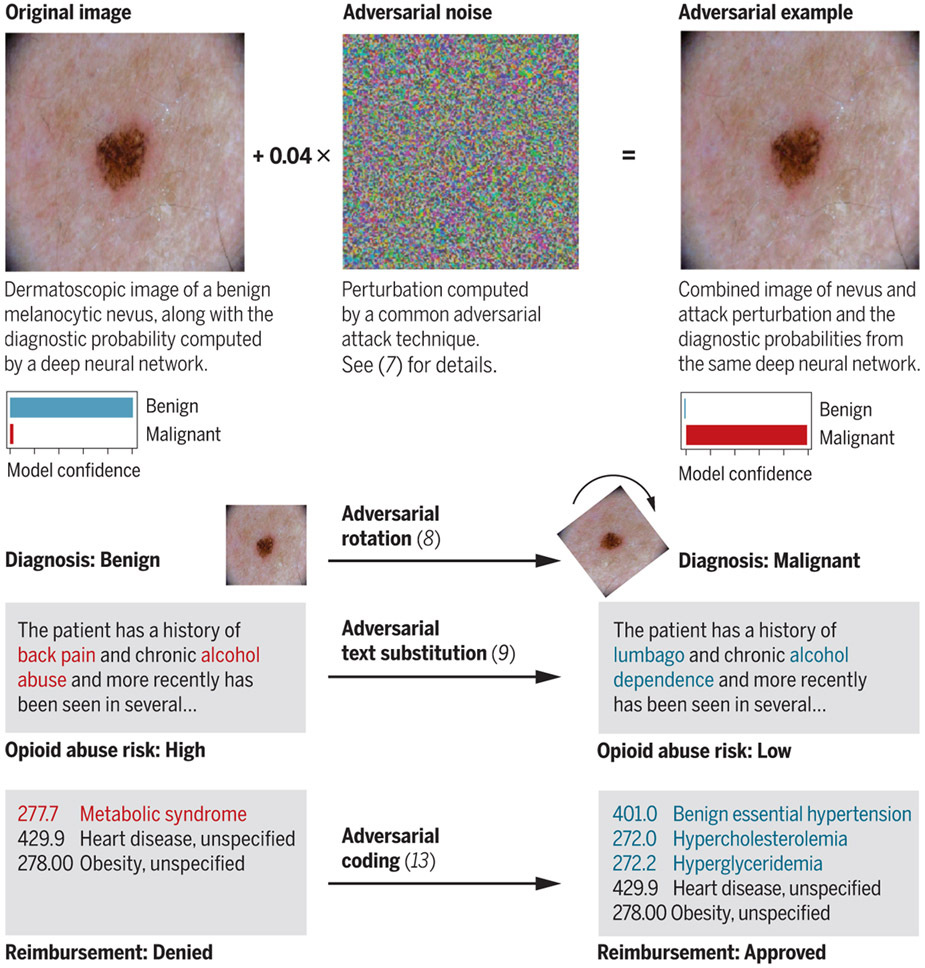
\includegraphics[width=0.65\linewidth]{figures/medical-adversarial-attacks.jpeg}
        \caption{Adversarial examples in health from Finlayson et al. (2019) \cite{finlayson_adversarial_2019}.}
        \label{fig:medical_adversarial_attacks}
    \end{figure}
    % \vspace*{-0.5cm}

    Furthermore, adversarial examples shine a light on the black-box nature of several types of ML models. The fact that these models can be fooled by small changes that are not perceptible to any expert raises questions about their general reliability and trustworthiness. This is why this phenomenon is an active area of research in the field \cite{finlayson_adversarial_2019}.

    One way to deal with adversarial attacks is by choosing models that are more robust to these examples. Goodfellow et al. 2015, for example, favor the use of nonlinear model families like RBF networks or using regularization strategies like dropout, weight decay, or gradient masking to improve the robustness of the model \autocite{goodfellowExplainingHarnessingAdversarial2015}.
    
    Another popular approach to make ML models more robust to these attacks is to feed adversarial examples directly into their training data. This is known as \textit{adversarial training}. Methods like the Fast Gradient Sign Method \cite{goodfellowExplainingHarnessingAdversarial2015} (FGSM) or the more recent Projected Gradient Descent (PGD) \autocite{madryDeepLearningModels2019}  can be used to generate adversarial examples and train the model to be robust to them. 

    % \subsection{Dynamic Quantization and Network Pruning} \label{sec:dynamic_quantization_pruning_sparsification} 
    % \info{0.5 pages}

    \todo[inline]{Modify this description and add more details, references \dots}

    \end{document}